 %	Main Document

\documentclass[
	12pt,
	BCOR=5mm,
	DIV=12,
	headinclude=on,
	footinclude=off,
	parskip=half,
	bibliography=totoc,
	listof=entryprefix,
	toc=listof,
	pointlessnumbers,
	plainfootsepline]{scrreprt}

% include configuration file
% !TEX root =  master.tex

% language, font, colors
\usepackage[ngerman]{babel}
\usepackage[utf8]{inputenc}
\usepackage[german=quotes]{csquotes} 	% correct quotes using \enquote{}
\usepackage[T1]{fontenc}
\usepackage{lmodern} % latin modern font
\usepackage[onehalfspacing]{setspace}
\usepackage{xcolor}

% hyperlinks
\PassOptionsToPackage{hyphens}{url}\usepackage[hidelinks=true]{hyperref}

% commands for author and title
\newcommand{\TitelDerArbeit}[1]{\def\DerTitelDerArbeit{#1}\hypersetup{pdftitle={#1}}}
\newcommand{\AutorDerArbeit}[1]{\def\DerAutorDerArbeit{#1}\hypersetup{pdfauthor={#1}}}
\newcommand{\Firma}[1]{\def\DerNameDerFirma{#1}}
\newcommand{\Kurs}[1]{\def\DieKursbezeichnung{#1}}


%\usepackage{microtype}% verbesserter Randausgleich
%\setlength\emergencystretch{1em}
% correct superscripts
\usepackage{fnpct}

\usepackage{footnote}
\usepackage{rotating}

% calc
\usepackage{calc} % Used for extra space below footsepline

% bibliography settings
% author-year-style with footnotes (Chicago)
\usepackage[backend=biber, autocite=footnote, style=authoryear, dashed=false]{biblatex}
\AdaptNoteOpt\footcite\multfootcite
\AdaptNoteOpt\autocite\multautocite

\DefineBibliographyStrings{ngerman}{  % change \ua to et al. (german only!)
	andothers = {{et\,al\adddot}},
}


% Command to output section title headings
\newcommand{\cvsect}[1]{% The only parameter is the section text
	\vspace{\baselineskip} % Whitespace before the section title
	\colorbox{black}{\textcolor{white}{\MakeUppercase{\textbf{#1}}}}\\% Section title
}

\newcounter{barcount}

% Environment to hold a new bar chart
\newenvironment{barchart}[1]{ % The only parameter is the maximum bar width, in cm
	\newcommand{\barwidth}{0.35}
	\newcommand{\barsep}{0.55}
	
	% Command to add a bar to the bar chart
	\newcommand{\baritem}[2]{ % The first argument is the bar label and the second is the percentage the current bar should take up of the total width
		\pgfmathparse{##2}
		\let\perc\pgfmathresult
		
		\pgfmathparse{#1}
		\let\barsize\pgfmathresult
		
		\pgfmathparse{\barsize*##2/5}
		\let\barone\pgfmathresult
		
		\pgfmathparse{(\barwidth*\thebarcount)+(\barsep*\thebarcount)}
		\let\barx\pgfmathresult
		
		\filldraw[fill=none, draw=black!] (0,-\barx) rectangle (5,-\barx-\barwidth);
		\filldraw[fill=black!90, draw=black!90] (0,-\barx) rectangle (\barone,-\barx-\barwidth);
		
		\node [label=180:{\textcolor{black}{##1: ##2/5}}] at (0,-\barx-0.175) {};
		\addtocounter{barcount}{1}
	}

	\newcommand{\baritemNL}[2]{ % The first argument is the bar label and the second is the percentage the current bar should take up of the total width
		\pgfmathparse{##2}
		\let\perc\pgfmathresult
		
		\pgfmathparse{#1}
		\let\barsize\pgfmathresult
		
		\pgfmathparse{\barsize*##2/5}
		\let\barone\pgfmathresult
		
		\pgfmathparse{(\barwidth*\thebarcount)+(\barsep*\thebarcount)}
		\let\barx\pgfmathresult
		
		\filldraw[fill=none, draw=black!] (0,-\barx) rectangle (5,-\barx-\barwidth);
		\filldraw[fill=black!90, draw=black!90] (0,-\barx) rectangle (\barone,-\barx-\barwidth);
		
		\node [label=180:{}] at (0,-\barx) {};
		\addtocounter{barcount}{1}
	}

	\begin{tikzpicture}
	\setcounter{barcount}{0}
}{
	\end{tikzpicture}
	\vspace{0.3cm}
}

\usepackage{tikz} % Required for creating the plots
\usetikzlibrary{shapes, backgrounds}
\tikzset{x=1cm, y=1cm} % Default tikz units

%%% Uncomment the following lines to support hard URL breaks in bibliography 
%\apptocmd{\UrlBreaks}{\do\f\do\m}{}{}
%\setcounter{biburllcpenalty}{9000}% Kleinbuchstaben
%\setcounter{biburlucpenalty}{9000}% Großbuchstaben

\setlength{\bibparsep}{\parskip}	% add some space between biblatex entries in the bibliography
\addbibresource{bibliography-martin.bib}	% add file bibliography.bib as biblatex resource
\addbibresource{bibliography-rene.bib}	% add file bibliography.bib as biblatex resource
\addbibresource{bibliography-sascha.bib}	% add file bibliography.bib as biblatex resource
\addbibresource{bibliography-niko.bib}	% add file bibliography.bib as biblatex resource
\addbibresource{bibliography-julian.bib}	% add file bibliography.bib as biblatex resource
\addbibresource{bibliography-erik.bib}	% add file bibliography.bib as biblatex resource
% footnotes (count footnotes over chapters)
\usepackage{chngcntr}
\counterwithout{footnote}{chapter}

% acronyms
\makeatletter
\usepackage[printonlyused]{acronym}
\@ifpackagelater{acronym}{2015/03/20}
  {%
    \renewcommand*{\aclabelfont}[1]{\textbf{\textsf{\acsfont{#1}}}}
  }%
  {%
  }%
\makeatother

% listings
\usepackage{listings}
\renewcommand{\lstlistingname}{Quelltext}
\renewcommand{\lstlistlistingname}{Quelltextverzeichnis}

%% More configuration for listings is in configlistings.tex %%


% extra packages
\usepackage{graphicx}			% use various graphics formats
\usepackage[german]{varioref}	% nicer references \vref
\usepackage{caption}			% better captions
\usepackage{booktabs}			% nicer tabs
\usepackage{array}
\usepackage{pdfpages}			% for signed ewerkl
%\usepackage{import}				% better import of section in several files
\usepackage{subfigure}

% table stuff
\newcolumntype{L}[1]{>{\raggedright\let\newline\\\arraybackslash\hspace{0pt}}m{#1}} % combines l and p
\newcolumntype{C}[1]{>{\centering\let\newline\\\arraybackslash\hspace{0pt}}m{#1}} % combines c and p
\newcolumntype{R}[1]{>{\raggedleft\let\newline\\\arraybackslash\hspace{0pt}}m{#1}} % combines r and p

% funktioniert aktuell nicht wie normal -> muss man nochmal drüber schauen.. oder ersetzen
\usepackage{tabularx}
\newcolumntype{Y}{>{\centering\arraybackslash}X}
\newcolumntype{b}{X}
\newcolumntype{s}{>{\hsize=.5\hsize\raggedleft\arraybackslash}X}
\newcolumntype{k}{>{\hsize=.5\hsize\arraybackslash}X}
\newcolumntype{r}{>{\raggedright\arraybackslash}X}

% page header/footer
\RequirePackage{scrlfile}
\ReplacePackage{scrpage2}{scrlayer-scrpage}
\RequirePackage[automark,headsepline,footsepline]{scrpage2}
\pagestyle{scrheadings}
\renewcommand*{\pnumfont}{\upshape\sffamily}
\renewcommand*{\headfont}{\upshape\sffamily}
\renewcommand*{\footfont}{\upshape\sffamily}
\renewcommand{\chaptermarkformat}{}
\RedeclareSectionCommand[beforeskip=0pt]{chapter}
\clearscrheadfoot

\ifoot[\rule{0pt}{\ht\strutbox+\dp\strutbox}DHBW Mannheim]{\rule{0pt}{\ht\strutbox+\dp\strutbox}DHBW Mannheim}
\ofoot[\rule{0pt}{\ht\strutbox+\dp\strutbox}\pagemark]{\rule{0pt}{\ht\strutbox+\dp\strutbox}\pagemark}

\ohead{\headmark}

% highlight notes as not yet finished
\newenvironment{note}{\color{gray}}{}

\usepackage{todonotes}
\usepackage{xspace}% http://ctan.org/pkg/xspace
\usepackage{fontawesome5}
\usepackage{float} % !important for figure position

% !TEX root =  master.tex

% colors
\definecolor{javared}{rgb}{0.6,0,0} % for strings
\definecolor{javagreen}{rgb}{0.25,0.5,0.35} % comments
\definecolor{javapurple}{rgb}{0.5,0,0.35} % keywords
\definecolor{javadocblue}{rgb}{0.25,0.35,0.75} % javadoc

\colorlet{jsonPunct}{red!60!black}
\definecolor{jsonBackground}{HTML}{EEEEEE}
\definecolor{jsonDelim}{RGB}{20,105,176}
\colorlet{jsonNumb}{magenta!60!black}

\definecolor{xmlGray}{rgb}{0.4,0.4,0.4}
\definecolor{xmlDarkblue}{rgb}{0.0,0.0,0.6}
\definecolor{xmlCyan}{rgb}{0.0,0.6,0.6}

\definecolor{jsBackground}{RGB}{250,250,255}
\definecolor{jsString}    {RGB}{ 16,160, 60}

\definecolor{cssKeyword}{RGB}{ 10,100,160}
\definecolor{cssClass}  {RGB}{200,120, 10}

% general style
\lstset{
	basicstyle=\ttfamily\footnotesize,
	backgroundcolor=\color{jsBackground},
	numbers=left,
	numberstyle=\scriptsize\color{black},
	stepnumber=1,
	numbersep=10pt,
	showspaces=false,
	showstringspaces=false,
	breaklines=true,
	tabsize=2,
	captionpos=b,
	literate=
	{Ö}{{\"O}}1
	{Ä}{{\"A}}1
	{Ü}{{\"U}}1
	{ß}{{\ss}}1
	{ü}{{\"u}}1
	{ä}{{\"a}}1
	{ö}{{\"o}}1
}

% Java
\lstdefinestyle{lstJava}
{
	language=Java,
	keywordstyle=\color{javapurple}\bfseries,
	stringstyle=\color{javared},
	commentstyle=\color{javagreen},
	morecomment=[s][\color{javadocblue}]{/**}{*/},
	tabsize=1
}

% JSON
\lstdefinelanguage{json}{
	literate=
	*{0}{{{\color{jsonNumb}0}}}{1}
	{1}{{{\color{jsonNumb}1}}}{1}
	{2}{{{\color{jsonNumb}2}}}{1}
	{3}{{{\color{jsonNumb}3}}}{1}
	{4}{{{\color{jsonNumb}4}}}{1}
	{5}{{{\color{jsonNumb}5}}}{1}
	{6}{{{\color{jsonNumb}6}}}{1}
	{7}{{{\color{jsonNumb}7}}}{1}
	{8}{{{\color{jsonNumb}8}}}{1}
	{9}{{{\color{jsonNumb}9}}}{1}
	{:}{{{\color{jsonPunct}{:}}}}{1}
	{,}{{{\color{jsonPunct}{,}}}}{1}
	{\{}{{{\color{jsonDelim}{\{}}}}{1}
	{\}}{{{\color{jsonDelim}{\}}}}}{1}
	{[}{{{\color{jsonDelim}{[}}}}{1}
	{]}{{{\color{jsonDelim}{]}}}}{1}
}

% XML
\lstdefinelanguage{XML}
{
	morestring=[b]",
	morestring=[s]{>}{<},
	morecomment=[s]{<?}{?>},
	stringstyle=\color{xmlGray},
	identifierstyle=\color{xmlDarkblue},
	keywordstyle=\color{xmlCyan},
	morekeywords={xmlns,version,type}
}

% JavaScript
\lstdefinelanguage{JavaScript}
{
	backgroundcolor=\color{jsBackground},
	keywordstyle=\color{blue}\bfseries,
	stringstyle=\color{jsString},
	commentstyle=\color{gray},
	morestring=[b]",
	morecomment=[l][\color{gray}]{//},
	morecomment=[s][\color{gray}]{/*}{*/},
	morekeywords={break,case,const,continue,else,false,for,function,if,in,new,null,switch,this,true,var,while}
}

% HTML
\lstdefinestyle{lstHTML}
{
	language=HTML,
	keywordstyle=\color{blue}\bfseries,
	commentstyle=\color{gray}\itshape,
	morecomment=[s][\color{gray}]{<!--}{-->},
%	stringstyle=\color{jsString}
	escapeinside=``
}

% CSS
\lstdefinestyle{lstCSS}
{
	keywordstyle=\color{cssKeyword}\bfseries,
	commentstyle=\color{gray}\itshape,
	morecomment=[s][\color{gray}]{/*}{*/},
%	morecomment=[s][\color{cssClass}]{.}{ \{},
	alsoletter=-,
	morekeywords={border,background-color}
}

%lstinline
\def\jinline{\lstinline[basicstyle=\ttfamily,keywordstyle={}, language=JAVA]}
\def\sinline{\lstinline[basicstyle=\ttfamily,keywordstyle={}, language=SQL]}

% !TEX root =  master.tex

\newcommand{\authorSG}{Sascha Görnert}
\newcommand{\authorNL}{Niko Lockenvitz}
\newcommand{\authorRF}{Rene Fischer}
\newcommand{\authorEJ}{Erik Jansky}
\newcommand{\authorGP}{Gerrit Pollkläsener}

\begin{document}

% set some information (title, author, ...)
\TitelDerArbeit{Entwurf und Implementierung eines Kinoreservierungssystems}
\AutorDerArbeit{\authorSG, \authorRF, \authorGP, \authorEJ, \authorNL}
\Firma{DER Touristik GmbH, Technische Universität Kaiserslautern, SAP SE}
\Kurs{WWI 17 SE B}

\begin{titlepage}

\begin{minipage}{\textwidth}
	\vspace{-2cm}
	\noindent
	
\includegraphics[height=0.1\linewidth]{img/logos/der}
	\hfill
	
\includegraphics[height=0.1\linewidth]{img/logos/tukl}
	\hfill
	
\includegraphics[height=0.1\linewidth]{img/logos/sap}
	\hfill
	
\includegraphics[height=0.1\linewidth]{img/logos/dhbw}
\end{minipage}

\vspace{1em}
\sffamily

\begin{center}
	\textsf{\large{}Duale Hochschule Baden-Württemberg\\[1.5mm] Mannheim}\\[2em]
	\textsf{\textbf{\Large{}Seminararbeit}}\\[3mm]
	\textsf{\textbf{\DerTitelDerArbeit}}\\[1.5cm]
	\textsf{\textbf{\Large{}Studiengang Wirtschaftsinformatik}\\[3mm] \textsf{Studienrichtung Software Engineering}}
	
	\vspace{3em}
	\vfill

	\begin{minipage}{\textwidth}
	
		\begin{tabbing}
			Bearbeitungszeitraum: \hspace{0.85cm}\=\kill
			Verfasser: \> \authorSG, 2716910 \\
			\> DER Touristik GmbH \\
			\> \\
			\> \authorRF, 8703049 \\
			\> Technische Universität Kaiserslautern \\
			\> \\
			\> \authorMS, 8857640 \\
			\> SAP SE \\
			\> \\
			\> \authorEJ, 5980253 \\
			\> SAP SE \\
			\> \\
			\> \authorNL, 1308674 \\
			\> SAP SE \\
			\> \\[1.5mm]
			Kurs: \> \DieKursbezeichnung \\[1.5mm]
			Bearbeitungszeitraum: \> 18.11.2019 -- 09.06.2020
	\end{tabbing}

	\end{minipage}

\end{center}

\end{titlepage}

\pagenumbering{roman}
\normalfont

% table of contents
\tableofcontents

% figures
\listoffigures

% tables
%\listoftables

% listings (source code)
\lstlistoflistings

% acronyms
\clearpage
\chapter*{Abkürzungsverzeichnis}
\addcontentsline{toc}{chapter}{Abkürzungsverzeichnis}

\begin{acronym}[A23456789012] % longest acronym for correct indentation
	\acro{A23456789012}{This is just for indentation}

	\acro{AJAX}{Asynchronous JavaScript and \acs{XML}}
	\acro{API}{Application Programming Interface}
	\acro{CRUD}{Create, Read, Update, Delete}
	\acro{CSS}{Cascading Style Sheets}
	\acro{DAO}{Data Access Object}
	\acro{DBMS}{Datenbankmanagementsystem}
	\acro{DOM}{Document Object Model}
	\acro{DTO}{Data Transfer Object}
	\acro{DOM}{Document Object Model}
	\acro{DB}{Datenbank}
	\acro{ER-Modell}{Entity-Relationship-Modell}
	\acro{FSK}{Freiwillige Selbstkontrolle der Filmwirtschaft}
	\acro{HTML}{Hypertext Markup Language}
	\acro{HTTP}{Hypertext Transfer Protocol}
	\acro{HTTPS}{Hypertext Transfer Protocol Secure}
	\acro{IDE}{Integrated Development Environment}
	\acro{JOSE}{\acs{JSON} Object Signing and Encryption}
	\acro{JPA}{Java Persistence \acs{API}}
	\acro{JS}{JavaScript}
	\acro{JSX}{JavaScript \acs{XML}}
	\acro{JPQL}{Java Persistence Query Language}
	\acro{JSON}{JavaScript Object Notation}
	\acro{JWE}{JSON Web Encryption}
	\acro{JWS}{JSON Web Signature}
	\acro{JWT}{JSON Web Token}
	\acro{MVC}{Model-View-Controller}
	\acro{ORM}{Objektrelationaler Mapper}
	\acrodefplural{ORM}{Objektrelationale Mapper}
	\acro{POJO}{Plain Old Java Object}
	\acro{PWA}{Progressive Web App}
	\acrodefplural{PWA}{Progressive Web Apps}
	\acro{QR-Code}{Quick Response Code}
	\acro{RDBMS}{Re\-la\-tio\-nal Database Management System}
	\acro{RFC}{Request for Comments}
	\acro{REST}{Representational State Transfer}
	\acro{SOA}{Service-Oriented Architecture}
	\acro{SPA}{Single-Page-Anwendung}
	\acrodefplural{SPA}{Single-Page-Anwendungen}
	\acro{SQL}{Structured Query Language}
	\acro{URI}{Uniform Resource Identifier}
	\acro{URL}{Uniform Resource Locator}
	\acro{URN}{Uniform Resource Name}
	\acro{UX}{User Experience}
	\acro{UI}{User Interface}
	\acro{XML}{Extensible Markup Language}
\end{acronym}

\ohead{Acronyms}

%--------------------------------
% Content
%--------------------------------
\clearpage
\ihead{\chaptername~\thechapter}
\ohead{\headmark}
\pagenumbering{arabic}

% one file for each chapter
% !TEX root =  master.tex
\chapter{Einleitung}

Diese Seminararbeit beschreibt das im Umfang des Moduls Fallstudie entwickelte Kinoreservierungssystem der Gruppe um Sascha Görnert, Rene Fischer, Erik Jansky, Niko Lockenvitz und Gerrit Pollkläsener.
Zielsetzung des zu entwickelten Systems ist es, einem Nutzer die Online-Buchung eines (oder mehrerer) Kinotickets zu ermöglichen.
Eine genauere Erläuterung der eigens gesetzten Ziele sowie eine Betrachtung, inwiefern diese erreicht wurden, findet in Kapitel \vref{sec:ziele} statt.
In den folgenden Abschnitten werden die durchlaufenen Entwicklungsschritte, einschließlich Planungsphase, Umsetzung und Reflexion erläutert und spezifiziert.

% !TEX root =  master.tex
\chapter{Analyse}
\chaptermulitpleauthor{\authorSG}{\authorGP, \authorRF, \authorEJ}

% !TEX root =  master.tex
\section{Personas}
\label{sec:Personas}

% !TEX root =  master.tex
\subsection{Persona a}
% !TEX root =  master.tex
\newcommand{\ariane}{Ariane Aris\xspace}
% -------------------------------------------------------
% Studierende Person
%
% --------------------------------------------------------
\newpage
\cvsect{\ariane}
\begin{minipage}[t]{0.5\textwidth}
	\vspace{-3.6cm}
	\renewcommand{\arraystretch}{1.5}
	\begin{tabular}{l l}
		Name: & \ariane \\
		Alter: & 20 \\
		Tätigkeit: & Studentin der Wirtschaftsinformatik \\
		Skills: & 3/5 \hspace{-1cm} \begin{barchart}{5.0}
			\baritemNL{}{3}
		\end{barchart} \\
	\end{tabular}
\end{minipage}
\hfill
\begin{minipage}[t]{0.4\textwidth}
	\flushright
	\includegraphics[width=0.70\textwidth]{img/personas/ariane}
\end{minipage}
\autocite{rf-unsplash-studentin}

Das möchte ich gerne haben:
\begin{itemize}
	\item einfaches, schnelles und unkompliziertes Erstellen neuer Umfragen für ihre wissenschaftlichen Arbeiten
	\item Auswertung der Umfrageergebnisse
    \item Teilnahme an anderen Umfragen
\end{itemize}

Mit der zweiten Persona, \ariane, wird eine Studentin für Wirtschaftsinformatik einer Hochschule beschrieben.
\ariane nimmt primär die Rolle einer Umfrageerstellerin und sekundär die Rolle einer Teilnehmerin ein.
Dabei möchte sie sowohl einfach eine Umfrage erstellen, als auch bei anderen Umfragen teilnehmen können.
% !TEX root =  master.tex

% -------------------------------------------------------
% umfrageteilnehmende Person
% -------------------------------------------------------
\newpage
\cvsect{Julian Weigert}
\begin{minipage}[t]{0.5\textwidth} 	\vspace{0.2\baselineskip} % Required for vertically aligning minipages
	\begin{entrylist}
		\entry
		{Name:}
		{Julian Weigert}
			\entry
		{Alter:}
		{24}
		\entry
		{Tätigkeit:}
		{Student für BWL}
	\end{entrylist}
	\begin{barchart}{5.0}\hspace{-1mm}
		\baritem{Skills}{2}
	\end{barchart}
\end{minipage}
\hfil
\begin{minipage}[t]{0.4\textwidth} 	\vspace{0.0\baselineskip} % Required for vertically aligning minipages
	\flushright
	\includegraphics[width=0.70\textwidth]{img/personas/julian}
\end{minipage}
\autocite{rf-unsplash-student}

Das möchte ich gerne haben:
\begin{itemize}
	\item Umfragen anonym durchführen
    \item Umfragen auf seinem Smartphone durchführen
    \item Umfragen auch später durchführen
\end{itemize}

Mit der dritten Persona, Julian Weigert, wird ein technisch weniger begabter Student einer Hochschule beschrieben.
Julian Weigert nimmt primär die Rolle des Umfrageteilnehmers ein, wobei er die Umfragen gerne an seinem mobilen Endgeräten bearbeiten möchte.
Durch seinen eng getakteten Zeitplan möchte er Umfragen auch Tage nach der Herausgabe des Links beantworten können.


% !TEX root =  master.tex
\section{User-Stories}
\multipleauthorsection{\authorGP}{\authorRF, \authorEJ}

Mit der großen Spannbreite an Personas gibt es auch zahlreiche, teils sich stark unterscheidende Anforderungen an das Kinobuchungssystem.
Im folgenden Abschnitt werden diese Wünsche der Personas aufgezählt und gruppiert.

\subsection{Übersicht / Filmauswahl}
Zuerst werden die Anforderungen an eine Übersicht über das aktuelle Filmprogramm geschildert.

\cvsect{Florentina Kastenkette}
Als Florentina Kastenkette interessiere ich mich primär nur für eine schnelle Übersicht der neuesten und beliebtesten Filme.

\cvsect{Leon Schweickert}
Als Leon Schweickert finde ich eine ausführliche Auflistung aller Filme geeigneter, um mich über alle Filme genauer zu informieren und somit die Besetzung und Vorschau eines Films ansehen zu können oder auch die Beschreibung des Films zu lesen.
\\
Als Leon Schweickert würde ich mich für einen E-Mail-Newsletter mit dem Kinoprogramm interessieren, um immer auf dem Laufenden zu bleiben.

\cvsect{Familie Mandick}
Als Familie Mandick legen wir einen großen Wert darauf, dass wir das vielfältige Filmprogramm nach Genre oder \acs{FSK}-Bewertung filtern können, um auch für unsere Kinder geeignete Filme zu finden.
\\
Als Familie Mandick möchten wir eine vereinfachte Suche nach Filmen, um auch spontan das Kino besuchen zu können.

\cvsect{Oma Gertrud}
Als Oma Gertrud möchte ich Werbung zu neuen Kinofilmen als Zeitungsan\-non\-ce sehen, um immer auf dem neuesten Stand zu sein.

\subsection{Auswahl einer Vorstellung}
Nach der Auswahl eines Films folgt die Wahl einer Vorstellung (Zeit und Datum).

\cvsect{Johnny Cash}
Als Johnny Cash möchte ich eine klare Übersicht der nächsten Vorstellungen, um so schnell wie möglich den passenden Termin für die Kunden zu finden.

Als Johnny Cash möchte ich nach zukünftigen Vorstellungen suchen und filtern können, um den Kunden bei der Reservierung dieser zu helfen.

\cvsect{Leon Schweickert}
Als Leon Schweickert möchte ich bereits auf der Übersicht die nächsten Vorstellungen zu den Blockbustern sehen, um Zeit beim Buchungsvorgang zu sparen.

\cvsect{Florentina Kastenkette}
Als Florentina Kastenkette möchte ich eine Detailseite der Filme mit allen Vorstellungen, um mit meinen Freundinnen den Kinobesuch perfekt planen zu können. \\
Als Florentina Kastenkette möchte ich schnell erkennen oder filtern können, welche Vorstellungen in 2D bzw. 3D sind, und ob die Filme in deutscher Sprache oder in ihrer Originalfassung aufgeführt werden, um nicht beim Kinobesuch enttäuscht zu werden.

\cvsect{Oma Gertrud}
Als Oma Gertrud möchte ich im Kino anrufen und mir Vorstellungen von einem Mitarbeiter ansagen und anschließend einen Platz auf meinen Namen reservieren lassen.

\subsection{Sitzplatzauswahl}
\cvsect{Florentina Kastenkette}
Als Florentina Kastenkette möchte ich mehrere Plätze mit unterschiedlichen Ermäßigungsstufen auswählen zu können, um auch mal mit meiner minderjährigen Schwester ins Kino gehen zu können.

\cvsect{Leon Schweickert}
Als Leon Schweickert möchte ich eine hübsche grafische Platzauswahl, bei der man auf einen Blick zwischen belegten und unbelegten Plätzen unterscheiden kann, sodass ich beim Buchen keine Zeit mit der Platzsuche verschwenden muss.

\cvsect{Johnny Cash}
Als Johnny Cash möchte ich, dass Reservierungen und Buchungen von mir eine höhere Priorität haben als die der Online-Nutzer, um den Kunden vor Ort ein angenehmes Kinoerlebnis zu ermöglichen.

\subsection{Bezahlung}
\cvsect{Oma Gertrud}
Als Oma Gertrud möchte ich meine Tickets nur reservieren und später im Kino bar bezahlen, um nicht meine Kreditkartendaten im Internet freizugeben.

\cvsect{Florentina Kastenkette}
Als Florentina Kastenkette möchte ich vor Ort bezahlen können, um meine Ausgaben auf der Kreditkartenabrechnung sehen zu können.

\cvsect{Leon Schweickert}
Als Leon Schweickert möchte ich online per PayPal bezahlen und dies auch in meinem Nutzerkonto als bevorzugtes Zahlungsmittel hinterlegen können, um nicht bei jeder Buchung meine Daten neu einzugeben.

\cvsect{Johnny Cash}
Als Johnny Cash möchte ich eine möglichst große Auswahl an Bezahlungsmöglichkeiten anbieten, um den Bezahlvorgang so unproblematisch wie möglich zu gestalten.
\\
Als Johnny Cash möchte ich die Gesamtpreise berechnet bekommen, um so schnell den Preis dem Kunden sagen zu können.

\subsection{Bestätigung}
\cvsect{Leon Schweickert}
Als Leon Schweickert möchte ich neben einer allgemeinen Bestätigung auf der Webseite, die Tickets auch auf meinem Smartphone erhalten, um für meinen Kinobesuch nichts ausdrucken zu müssen. \\
Als Leon Schweickert möchte ich außerdem, dass die Webseite auch auf meinem Smartphone schön dargestellt werden kann, damit ich schnell von unterwegs Tickets buchen kann.

\cvsect{Florentina Kastenkette}
Als Florentina Kastenkette möchte ich meine Buchung direkt in meinen sozialen Netzwerken teilen, um meine Freunde und Follower immer auf dem neusten Stand zu halten. \\
Als Florentina Kastenkette möchte ich nur ein gemeinsames Ticket für alle meine Freunde haben, damit ich es nicht koordinieren muss, jedem sein persönliches Ticket zu schicken.

\subsection{Reservierungsbearbeitung}
\cvsect{Familie Mandick}
Als Familie Mandick möchten wir unsere gebuchten Tickets auch noch spontan stornieren können, da bei uns schnell mal etwas dazwischen kommt.

\cvsect{Leon Schweickert}
Als Leon möchte ich meine Reservierungen oder gekauften Tickets per Knopfdruck in meinen (mobilen) Kalender übertragen können, wobei ich gern auch noch eine eigene Notiz anhängen können würde.

\subsection{Im Kino}
\cvsect{Oma Gertrud}
Als Oma Getrud möchte ich mein Ticket an der Kasse erhalten, dies ist für mich als Oma Gertrud sehr wichtig, da ich gern ein Stück Papier vorzeigen können möchte.

\cvsect{Johnny Cash}
Als Johnny ist es mir wichtig, schnell auf online reservierte Tickets an der Kasse zugreifen zu können, damit Kunden online reservieren und an der Kasse bezahlen können.

\cvsect{Familie Mandick \& Leon Schweickert}
Als Familie Mandick oder auch Leon Schweickert wollen wir den Schritt an der Kasse überspringen und direkt den Weg Richtung Kinosaal antreten.
Als Leon möchte ich die gesparte Zeit durch die Onlinebuchung verwenden, um Snacks für das Kino zu kaufen.
Als Familie Mandick möchte wir nur eine kurze Zeit in der Warteschlange verbringen, um die Kinder vor dem Kinoerlebnis nicht mit unnötiger Warterei zu foltern.
Ebenfalls möchten wir die Möglichkeit haben, um so spät wie möglich zu einem Kinofilm anzukommen.

\cvsect{Florentina Kastenkette \& Leon Schweickert}
Als einer der beiden jungen Nutzer (Florentina oder Leon) möchte ich meinen Studentenausweis bzw. Schülerausweis in meinem Benutzerprofil hinterlegen, um diesen nicht bei jedem Kinobesuch vorzeigen zu müssen.

\subsection{Sonstiges}
Die sonstigen Wünsche beziehen sich hauptsächlich auf häufige Besucher und Webseiten-Nutzer wie Leon.

Als Leon Schweickert möchte ich Filter speichern, um die Webseite zu individualisieren und noch schneller nutzen zu können.
Ebenso wünsche ich mir eine Einsicht in meine Historie und Statistik, damit ich sehen kann, wie oft ich ins Kino gehe. \\
Als Leon Schweickert möchte ich außerdem Bewertungen und Kommentaren für Filme erstellen, da ich als erfahrener Kinobesucher gerne anderen Personen helfen möchte, gute Filme auszuwählen.

Außerdem wäre es für mich als Leon nützlich, von Rabattaktionen oder Bonusprogrammen profitieren zu können, da ich so oder so viel Zeit im Kino verbringe.

% !TEX root =  ../../master.tex
\section{User-Journey}
%\label{sec:user_journey}
%Anhand der nun weitestgehend geschilderten Anforderungen aller Personas wurde der Aufbau der Website für das entwickelte Kinobuchungssystem entschieden.
%Diese gewählte Struktur wird im Folgenden anhand eines Beispiels geschildert, in welchem ein Endnutzer drei Tickets für eine spezielle Filmvorführung bucht.
%Vorausgesetzt ist hierbei, dass der Nutzer tatsächlich eine Online-Buchung vornimmt und nicht direkt im Kino anruft, um ein Ticket zu erwerben bzw. einen Sitzplatz zu reservieren.
%
%\begin{figure}[ht]
%	\centering
%	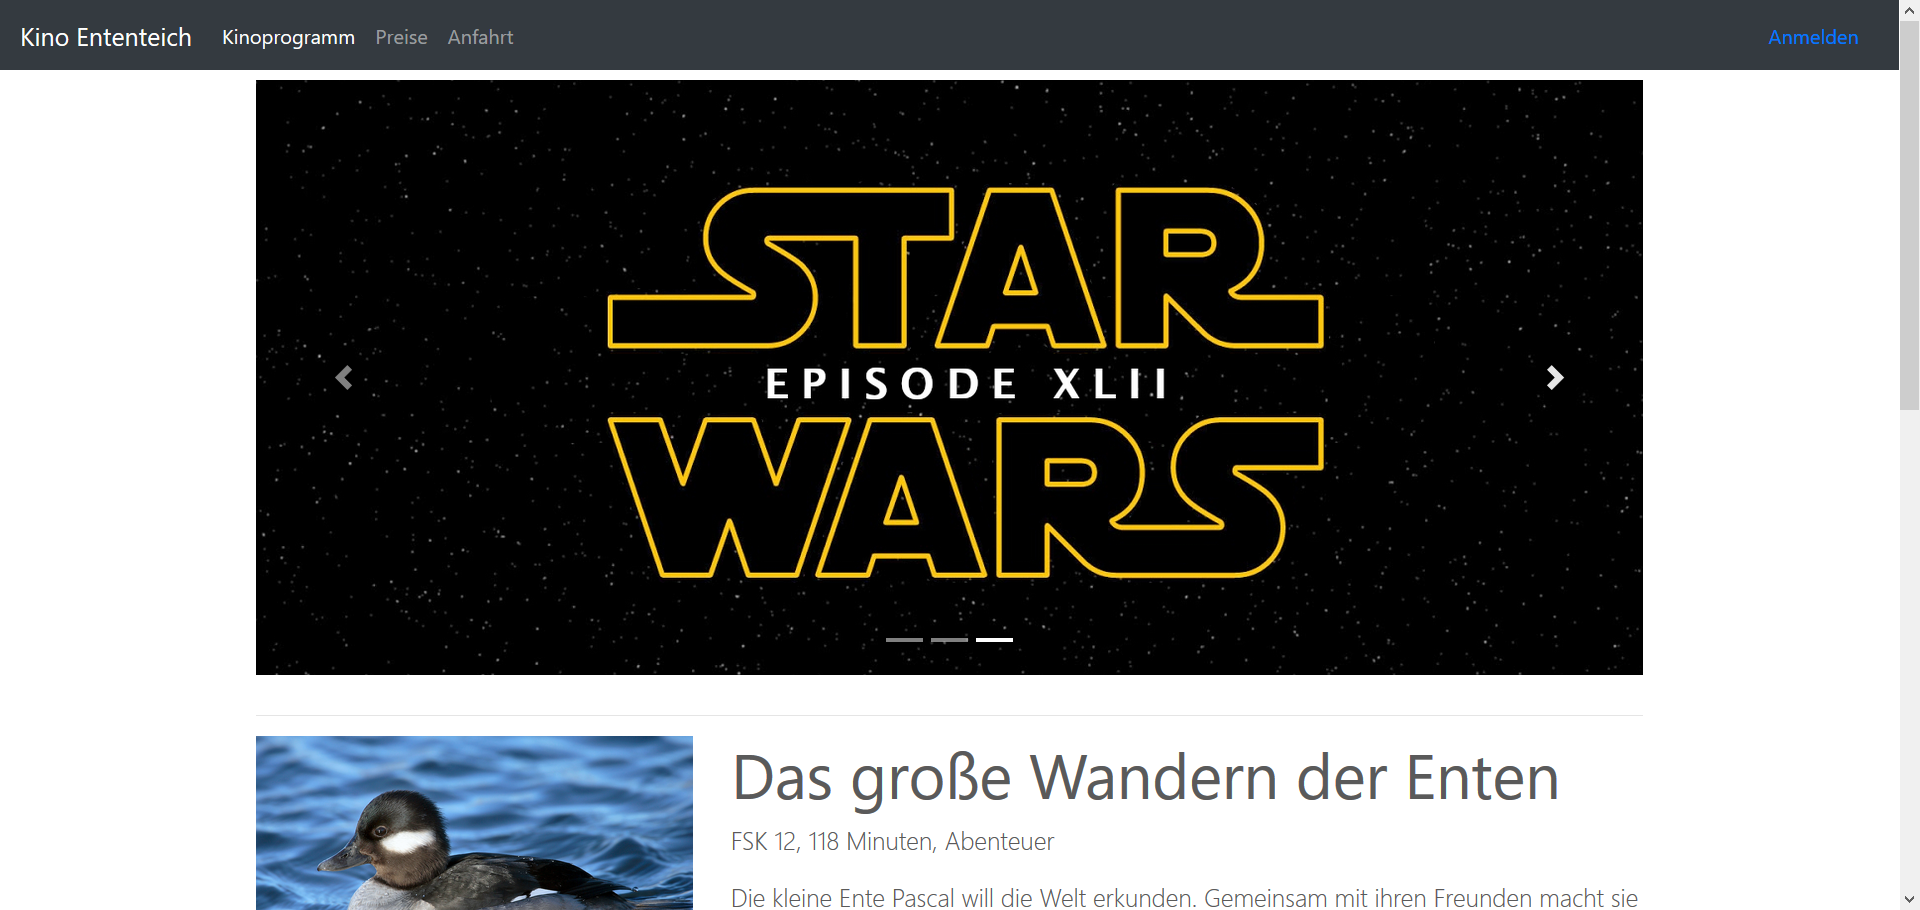
\includegraphics[width=\textwidth]{img/screenshots/startseite00}
%	\captionsetup{format=hang}
%	\caption{Startseite}
%	\label{fig:startseite00}
%\end{figure}
%
%Bei Aufruf der Startseite des Kinos wird dem Nutzer eine Übersicht über alle momentan im Kino laufenden Filme präsentiert.
%Ganz oben befindet sich dabei ein Karussell mit den beliebtesten Filmen.
%Darunter ist eine Liste mit allen Filmen.
%Durch Herauf- und Herabscrollen lässt sich schnell durch diese Liste navigieren, das Finden des gesuchten Films wird durch die großen Cover-Bilder neben dem Titel erleichtert.
%Durch Anwählen des Filmtitels wird der Nutzer auf die Seite für diesen Film geleitet, auf der alle Vorstellungen des Films innerhalb der nächsten Tage aufgelistet sind.
%Dort findet sich auch eine detaillierte Beschreibung und eine Bewertung des Films durch andere Benutzer (vgl. Anhang \vref{sec:screenshots_frontend}).
%
%Eine jede dieser Vorstellungen ist durch einen Knopf in der nach Tagen geordneten Tabelle repräsentiert, mit der passenden Uhrzeit als Beschriftung.
%Wurde der Knopf mit dem gewünschten Vorstellungszeitpunkts ausgewählt, so wird der Nutzer zur Sitzplatzübersicht und -auswahl weitergeleitet.
%
%Als nächstes ist für den Anwender die Wahl der Sitzplätze relevant.
%Dies geschieht im entwickelten Buchungssystem durch die Anwahl der Plätze in einer 2D-Grafik des Kinosaals, in welcher bereits belegte, freie und eigens angewählte Plätze farblich voneinander abgehoben sind.
%Nach der Auswahl der gewünschten Sitzplätze sollte der Nutzer nun in der Lage sein, die Preiskategorien der Plätze (Ermäßigungen usw.) auszuwählen und den Einzel- sowie Gesamtpreis der Auswahl einsehen zu können.
%
%\begin{figure}[ht]
%	\centering
%	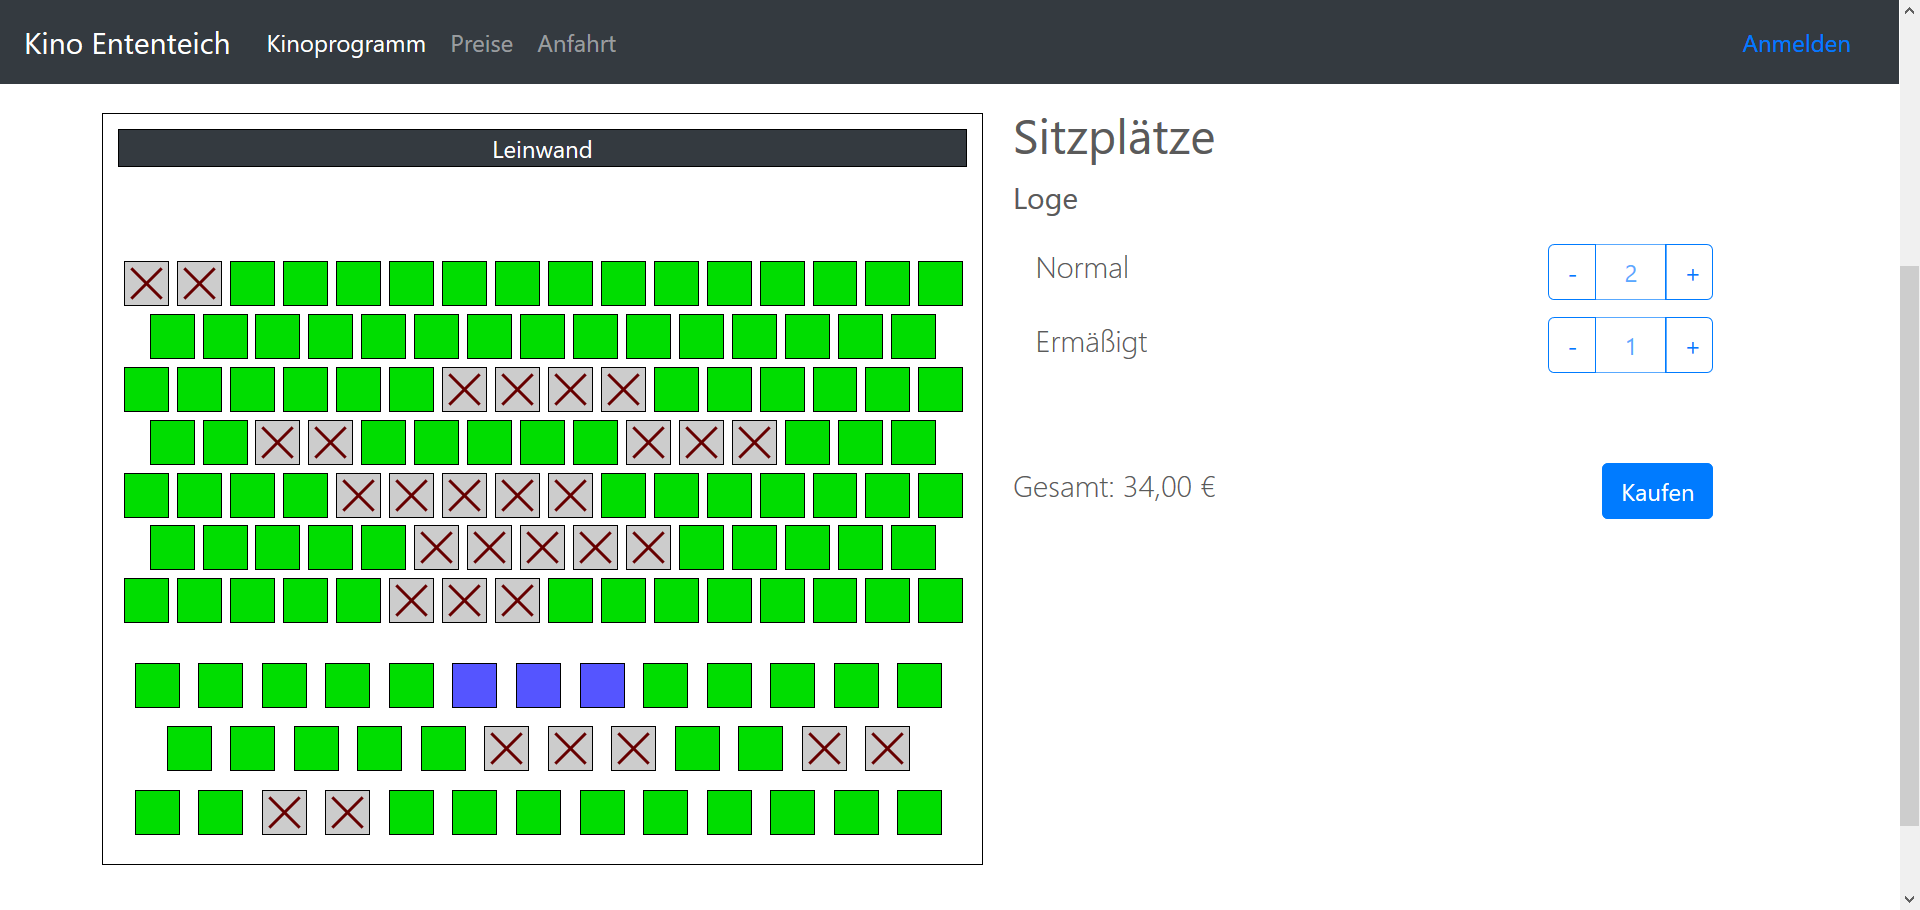
\includegraphics[width=\textwidth]{img/screenshots/vorstellung02}
%	\captionsetup{format=hang}
%	\caption{Auswahl der Sitzplätze}
%	\label{fig:vorstellung02-2}
%\end{figure}
%
%Ist der Nutzer mit diesem Schritt fertig, kommt es nun zum Bezahlvorgang für die ausgewählten Tickets.
%Hier soll der Nutzer eine kompakte Übersicht über die Bestellung erhalten, und nach Überprüfung seiner Auswahl seine persönlichen Daten (Vorname, Nachname und E-Mail-Adresse) angeben können.
%Drüber hinaus soll noch die Auswahl zwischen mehreren Zahlungsmethoden sowie die Eingabemöglichkeit für Rabattcodes angeboten werden.
%
%Mit der Zahlungsbestätigung ist der Nutzer im letzten Schritt des Buchungsvorgangs angelangt.
%Hier werden erneut die zusammengefassten Details der Bestellung (Kosten, Sitzplätze, Filmdetails und Vorstellungszeitpunkt) sowie ein Bestätigungstext angezeigt.
%Außerdem wird dem Nutzer sein digitales Ticket in Form eines \acs{QR-Code}s angezeigt, welches der Anwender auch per E-Mail zugesandt bekommt oder mithilfe eines Accounts in der mobilen App abrufen kann.
%Dieser Code enthält alle Infos über das Ticket und ist im Kino gleichwertig mit einer ausgedruckten Version.
%
%Neben diesem Anwendungsfall gibt es natürlich noch andere Berührungspunkte der Anwender mit dem System außerhalb der Aufgabenstellung dieser Arbeit.
%Hierzu zählen unter anderem eine Ticketbuchung bzw. -reservierung per Telefon sowie die Verarbeitung einer Buchung durch einen Kinomitarbeiter.
%Im Allgemeinen ähneln sich die Schritte insofern, dass Film-, Vorstellungs- und Sitzplatzauswahl vom Ablauf her gleich bleiben, für den Kinomitarbeiter jedoch kompakter dargestellt werden können.
%Filmbeschreibungen, Bewertungen, Titelbilder usw. spielen hier keine Rolle, da diese Informationen für den Mitarbeiter als Fachmann irrelevant sind.
% !TEX root =  master.tex
\section{Ablauf im Kino}

Der vorgesehene Ablauf im Kino lässt sich in 3 distinktive Arten unterteilen, die im Folgenden genauer beschrieben werden.

Zuerst wird ein Kinobesuch betrachtet, in welchem der Kunde keine Tickets im Voraus gekauft oder reserviert hat.
In diesem Falle würde der Kunde sich am Schalter über das aktuelle Kinoprogramm informieren und nach Auswahl eines Films, Vorstellungszeitpunkts und Sitzplatzes die Tickets kaufen.
Nun kann der Kunde mit seinen vom Verkäufer erhaltenen Tickets das passende Kino betreten und den auf dem Ticket angegebenen Sitzplatz einnehmen.
Die Ticketkontrolle findet dabei direkt vor dem Kinosaal statt, wo das Ticket vom Personal kontrolliert wird.
Optional kann er davor natürlich noch Getränke und Snacks an der Snackbar kaufen. 
Zusammengefasst gibt es also vor Ort 3 Schritte, die die meisten Gäste durchlaufen:
Ticketkauf am Schalter, Kauf von Snacks und Eintritt in den passenden Kinosaal.
Die Kinomitarbeiter müssen in diesem Fall einerseits das für den Kunden passende Ticket auswählen und verkaufen, andererseits aber auch die Snackbar besetzen und vor dem Kinosaal die Tickets überprüfen.

Etwas schneller läuft es ab, wenn der Kunde vorab seine Sitzplätze reserviert hat.
In einem solchen Szenario fällt der erste Schritt in der Kette kürzer aus:
Statt den Kunden zu beraten und Laufzeiten heraussuchen zu müssen, kann der Kinomitarbeiter am Schalter einfach per Reservierungsnummer oder Name die Tickets für die vorab gewählten Sitzplätze verkaufen.
Dies verkürzt allgemein die Bearbeitungszeit für einzelne Kunden, was zu kürzeren Wartezeiten am Schalter führt.
Der sonstige Ablauf bleibt jedoch weitestgehend gleich.

Der schnellste und einfachste Ablauf vor Ort bietet sich dann, wenn der Kunde bereits im voraus seine Tickets online erworben hat.
In diesem Fall wird der Schritt am Schalter obsolet.
Stattdessen können die Kunden direkt Snacks erwerben oder zum Kinosaal gehen, wo ihre entweder im Voraus ausgedruckten oder auf dem Handy gespeicherten Online-Tickets kontrolliert werden.
Bis auf den Vorgang am Schalter bleibt auch hier der sonstige Ablauf gleich, weshalb dieser Ablauftyp für sowohl Kinopersonal als auch Kunden am unkompliziertesten ist.

% !TEX root =  master.tex
\chapter{Entwurf}
\label{c:entwurf}

% !TEX root =  master.tex
\section{Klassendiagramm}
\label{sec:Klassendiagramm}
\multipleauthorsection{\authorSG}{\authorNL}

Das Klassendiagramm wurde im Verlauf des Projekts mehrfach angepasst.
Der erste Entwurf befindet sich in Anhang \vref{fig:anhang_klassendiagramm01}.
Die aktuelle Version ist in Anhang \vref{fig:anhang_klassendiagramm02} zu finden.

% !TEX root =  master.tex
\section{Sequenzdiagramm}
\label{sec:sequenzdiagram}
\authorsection{\authorSG}

Im Anhang \vref{fig:Anhang_seq_reservieren} befindet sich ein Sequenzdiagramm des Reservierungsvorganges.

Im Folgenden werden die einzelnen Schritte kurz erläutert.

Nachdem der Benutzer die gewünschten Sitzplätze ausgewählt hat, drückt er im Front-End auf den Button \enquote{Reservieren}.
Im Front-End wird daraufhin ein \acs{JSON} mit den Informationen der gewünschten Sitzplätze erstellt (siehe \vref{lst:json_book}).
Vor dem \acs{JSON} wird noch ein Formparameter book angeschlossen, um eine genauere Identifizierung in der \acs{REST}-Schnittstelle \jinline|reservation/book| zu realisieren.

Das Front-End ruft über einen \acs{AJAX}-Call den Webserver mit der \acs{URI}  \url{http://localhost:8080/cinemasystem-system/reservation/book} auf und übergibt dabei das \acs{JSON}.
Diese Ressource ruft ihren eigenen Service auf.
Dieser ruf den Webserver für die Datenschicht über die \acs{URI} \url{http://localhost:8080/cinemasystem-data/reservation/book} auf und übergibt das \acs{JSON}.
Hier wird das \acs{JSON} mittels eines \acs{JSON}-Converters in ein \acs{DTO} konvertiert.
Da aus dem Front-End lediglich die Vorstellungs-ID übermittelt wird, müssen die Informationen der Vorstellung aus der Datenbank nachgeladen werden. \\
Hier wird die Methode \jinline|find(String id)| im \jinline|ShowService|, der ebenfalls in der Ressource implementiert ist, aufgerufen.
Diese greift auf die Datenbank zu und holt die Informationen der Vorstellung ab und wandelt es anschließend in ein Show-\acs{DTO} um.

%Anschließend kann eine Verifizierung erfolgen, ob überhaupt eine Reservierung derzeit möglich ist.
%Ein möglicher Ausschlussgrund könnte sein, dass zwischen Beginn der ausgewählten Vorstellung und aktueller Zeit weniger als 30 Minuten liegen. \\
%Ist diese erfolgreich gewesen, wird überprüft, ob es bereits den Kunden in der Datenbank gibt.
%Dies wird durch die vom Front-End übermittelte E-Mail-Adresse des aktuellen Benutzers durchgeführt.
%Somit kann später der Reservierung und somit den Tickets eindeutig der Kunde zugewiesen werden. \\

Anschließend erfolgen verschiedene Verifizierungen, ob das Anlegen der Reservierung möglich ist.
Ausschlussgründe könnten etwa folgende sein:
\begin{enumerate}
	\item Zwischen Vorstellung und aktueller Uhrzeit liegen weniger als 30 Minuten.
	\item Der ausgewählte Sitzplatz ist schon von einem anderen Benutzer blockiert.
	\item Der ausgewählte Sitzplatz ist bereits vergeben.
\end{enumerate}
War die Reservierung erfolgreich, wird das Ergebnis an den \jinline|ReservationService| des Webserver System im \acs{JSON} zurück übermittelt. % TODO: Webserver? Webservice?
Ggf. kann es hier noch zu weiteren Berechnungen kommen, weshalb das \acs{JSON} in ein Reservation\acs{DTO} umgewandelt wird.

Ist die Methode \jinline|postTickets| abgeschlossen, wird das Ergebnis in ein \acs{JSON} umgewandelt und an das Front-End gesendet, welches dem Benutzer die Reservierung als \acs{QR-Code} darstellt (siehe Kapitel \vref{fig:vorstellung04}).

Eine nähere Beschreibung der Herausforderungen für das Reservieren und den Lösungsansätzen befindet sich in Kapitel \vref{ssec:herausforderung_reservieren} und Kapitel \vref{ssec:loesung_reservieren}.

% !TEX root =  ../../../master.tex
\subsection{Authentifizierung}
\label{sec:authentifizierung}

Um einen angemessen Schutz der gespeicherten Daten zu gewährleisten, soll jeder Benutzer nur seine eigenen Daten einsehen können.
Ebenso sind auch die ausführbaren Aktionen auf den Benutzer zu beschränken, auf den sich diese beziehen.
Dies bedeutet, dass ein angemeldeter Benutzer nur die Ergebnisse seiner eigenen Umfragen sehen kann, nicht aber die Ergebnisse von Umfragen anderer Benutzer.

Daher muss ein Benutzer vom System identifiziert werden können.
Die erstellten Umfragen können dann einer solchen digitalen Identität zugeordnet werden.
Zum Anlegen dieser digitalen Identität erfolgt eine Registrierung mit Nutzername und Passwort.
Zusätzlich muss gemäß Anforderung~\ref{Anf:A2} ein Registrierungsschlüssel angegeben werden, sodass lediglich befugte Personen Benutzer erstellen können.

Das geheime Passwort ist nur dem jeweiligen Nutzer bekannt, sodass dieser sich damit authentisieren kann.
Der Server speichert das Passwort in der Datenbank, damit bei einer Anmeldung geprüft werden kann, ob der Nutzer auch der ist, der er vorgibt zu sein.

Aus Sicherheitsgründen wird das Passwort allerdings nicht im Klartext gespeichert.
Andernfalls wären alle Nutzerpasswörter in der Datenbank für alle, die auf diese Zugriff haben, einsehbar.
Sowohl potenzielle Angreifer, die möglicherweise durch Sicherheitslücken Zugang erhalten, als auch einfach die Betreiber der hier entwickelten Webanwendung hätten somit also Kenntnis von den Passwörtern aller Nutzer.
Dies ist insbesondere deswegen kritisch, da viele Nutzer dieselben oder ähnliche Passwörter bei mehreren Diensten verwenden.
Aufgrund der sich hieraus ergebenden Gefahren muss das Passwort also anders gespeichert werden.

Hierbei hat sich in der Praxis das Speichern eines kryptographischen Hashwertes etabliert.
Eine kryptographische Hashfunktion bildet einen Text beliebiger Länge auf einen zufällig erscheinenden Text mit fixer Länge ab.
Es handelt sich dabei um eine deterministische Einwegfunktion.
Das heißt, wenn derselbe Text, also hier dasselbe Passwort, in eine solche Funktion eingegeben wird, resultiert jedes Mal auch derselbe Hashwert.
Es ist allerdings nicht beziehungsweise nur mit einem enorm großen Aufwand möglich, die zu einem Hashwert gehörige Eingabe zu berechnen.

Das bedeutet für die Speicherung des Passworts, dass dieses praktisch nicht aus dem Hash ermittelt werden kann.
Bei einer Anmeldung kann die Korrektheit jedoch geprüft werden, indem der gespeicherte Hashwert mit dem Hash des eingegebenen Passworts abgeglichen wird.

Als weitere Sicherheitsmaßnahmen werden Salt und Pepper genutzt.
Dabei handelt es sich um weitere zufällige Zeichenketten, die dem Passwort angehangen werden, um Angriffe zu erschweren.
Der Salt ist für jeden Benutzer spezifisch und wird neben dem Passworthash in der Datenbank gespeichert.
Dadurch ist es möglich, dass selbst wenn zwei Benutzer dasselbe Passwort gewählt haben, die Hashwerte verschieden sind.
Ebenso erschwert es das Knacken der Passworthashes, da ein Angreifer die Hashes nicht im Voraus berechnen kann.
Der Pepper ist für alle Nutzer derselbe und außerhalb der Datenbank gespeichert.
Dieser wird in einer Konfigurationsdatei definiert und entsprechend vom Programm geladen.
Dies erschwert ebenso Angriffe auf die Hashwerte, da ein Angreifer, der lediglich Zugang zur Datenbank hat, den Pepper nicht kennt, sodass das Knacken deutlich schwieriger wird.

Nutzer, die sich registriert oder angemeldet haben, erhalten eine sogenannte Session-ID.
Diese wird dann bei \acs{API}-Aufrufen zur Authentifizierung genutzt, sodass hier nicht jedes Mal, dass Passwort genutzt werden muss.

Sollte ein Nutzer sein Passwort vergessen, kann dieses von Administratoren zurückgesetzt werden.
Es muss danach allerdings, wie in Anforderung~\ref{Anf:A6} beschrieben, direkt wieder vom Nutzer geändert werden.

Wenn die Nutzung eines Registrierungsschlüssels von den Administratoren als zu unsicher angesehen wird, können Sie Nutzer gemäß Anforderung~\ref{Anf:A3} auch manuell erstellen.
Auch hier muss ein vom Administrator festgelegtes Passwort, wie in Anforderung~\ref{Anf:A5} gefordert, direkt beim nächsten Anmelden angepasst werden.

Auf der anderen Seite müssen sich Personen, die Umfragen beantworten, gemäß Anforderung~\ref{Anf:A14} nicht anmelden.
Entsprechend haben Sie nur eine sehr eingeschränkte Sicht.
Sie können auf Umfragen lediglich über einen zehnstelligen Code zugreifen.
Dadurch ist es auch nur schwer bis gar nicht möglich auf Umfragen zuzugreifen, die nicht mit einem geteilt wurden.

% !TEX root =  master.tex
\section{Sitzplatzauswahl und Blockierungen}
\authorsection{\authorNL}

Beim Reservierungsvorgang ist es essentiell, dass ein Sitzplatz nicht mehrfach reserviert wird.

Hier ein einfaches Beispiel:
Benutzer A besucht die Seite, wählt einen Film und eine Vorstellung aus.
Die Saalübersicht wird geladen, wobei Sitzplätze, die bereits reserviert sind, optisch hervorgehoben sind und nicht mehr ausgewählt werden können.
Etwa zur gleichen Zeit besucht Benutzer B die Seite.
Er wählt die selbe Vorstellung, sieht die gleiche Saalübersicht und wählt einen Platz aus: Reihe 4, Platz 2.
Benutzer B folgt daraufhin den weiteren Schritten, bezahlt seinen Sitzplatz und erhält eine Bestätigung, dass Reihe 4, Platz 2 erfolgreich von ihm gebucht wurde.
Auch Benutzer A hat Reihe 4, Platz 2 ausgewählt.
Zu dem Zeitpunkt als Benutzer A den Saalplan geladen hat, war die Reservierung von Benutzer B noch nicht abgeschlossen, sodass der Platz frei war.
Auch Benutzer A möchte nun das Ticket bezahlen, muss aber eine Fehlermeldung erhalten, damit das Ticket für Reihe 4, Platz 2 nicht doppelt verkauft wird.

Spätestens bei der verbindlichen Reservierung und der normalerweise folgenden Bestätigung muss eine Fehlermeldung erscheinen, wenn der Platz bereits belegt ist.
Im Idealfall wird der Nutzer aber schon früher benachrichtigt, wenn er einen Platz ausgewählt hat, der in der Zwischenzeit von einem anderen Benutzer reserviert wurde.

Der Fall, dass ein Platz durch einen anderen Benutzer reserviert wird, ist mit gewisser Wahrscheinlichkeit vorhersehbar.
Wählt ein Benutzer im Saalplan ein paar Plätze aus, so wird er vermutlich in den nächsten paar Minuten mit der Bezahlung fortfahren und die Plätze für sich reservieren.
In dem Moment, wo ein Benutzer einen Sitzplatz also nur auswählt, kann diese Information bereits in der Datenbank gespeichert werden.
Der Sitzplatz wird für diesen Benutzer zwar nicht reserviert, aber für einen kurzen Zeitraum vorgemerkt.
Will nun jemand einen Platz auf dem Saalplan auswählen, teilt er dies über die \acs{API} dem Back-End mit.
Nun gibt es mehrere mögliche Ergebnisse:
\begin{enumerate}
\item Der ausgewählte Sitzplatz ist bereits reserviert.
\item Der ausgewählte Sitzplatz ist bereits für einen anderen Benutzer vorgemerkt, könnte also in einigen Minuten wieder frei werden.
\item Der Sitzplatz ist weder reserviert, noch vorgemerkt.
Er wurde nun erfolgreich für den aktuellen Benutzer vorgemerkt.
\end{enumerate}

Dies kann nun dazu führen, dass ein Benutzer einen freien Saalplan angezeigt bekommt und beim Anklicken eines Platzes dieser nun nicht mehr als \enquote{frei}, sondern als \enquote{durch einen anderen Nutzer belegt} angezeigt wird.

Die zu der Reservierung zugehörigen Operationen auf der Datenbank müssen atomar ausgeführt werden, sodass die Reservierung entweder erfolgreich war oder eine Fehlermeldung den Benutzer informiert, dass die Reservierung fehlgeschlagen ist.

Alle Sicherheitsprüfungen müssen im Back-End ausgeführt werden.
Natürlich können auch einzelne Prüfungen im Front-End implementiert werden, diese helfen allerdings nur einem normalen Benutzer den Vorgang zu erleichtern.
Eine Absicherung bieten derartige Prüfung im Front-End nicht, da der clientseitig ausgeführte Quellcode logischerweise vom Client verändert werden kann und jeder Angreifer eine manipulierte Anfrage mit selbst gewählten Parametern an die \acs{API} schicken kann.

\chapter{Back-End}
\chapterauthor{Sascha Görnert}
\label{sec:backend}
\section{Technologien}
\label{sec:technologien}

Für das hier erstellte Kinoreservierungsprogramm wurde die Verwendung von Java\footnote{\url{https://java.com/de/download/} -- Version 8.0.141 verwendet} für das Back-End vorgegeben. 

Als Java-\acs{IDE} kommt Eclipse\footnote{\url{https://www.eclipse.org/} -- Version: Photon Release (4.8.0)} zum Einsatz, da es aus vorangegangenen Vorlesungen bekannt ist.
Für die Kommunikation zwischen den einzelnen Schichten der Drei-Schichten-Architektur kommen \acs{REST}ful-Webservices in Verbindung mit Jersey\footnote{\url{https://jersey.github.io/} -- Version 1.19.4} sowie \acp{DTO} zum Einsatz (Kapitel \vref{sec:dto}), die zwischen den einzelnen Schichten transferiert werden.

Um eine Datenhaltung und den Austausch von Informationen zu gewährleisten, wurde sich in dieser Arbeit für eine Postgres Datenbank entschieden.
Der Zugriff auf die Datenbank erfolgt mittels der \ac{JPA} in Verbindung mit EclipseLink (Kapitel \vref{ssec:jpa}).
% !TEX root =  master.tex
\section{Konzept}
\label{sec:konzept}

In diesem Projekt soll die Drei-Schichten-Architektur eingesetzt werden.
Sie dient dazu, die einzelnen Schichten (Datenhaltung, Fachkonzept und Benutzeroberfläche) zu separieren, sodass in zukünftigen Schritten ein Austausch der genutzten Benutzeroberfläche, Fachkonzeptschicht oder Datenbank möglich ist.

Wie zuvor in Kapitel \vref{sec:technologien} beschrieben, finden in diesem Projekt \acs{REST}ful Webservices Anwendung.
Da Webservices in der Realität u.a. aus Per"-for"-mance-Gründen auf unterschiedlichen Servern ausgeführt werden, wurde dies hier ebenfalls umgesetzt.
Zum Einsatz kommt ein System- und Data-Webservice.
Wie in Abbildung \vref{fig:konzept_backend} dargestellt ist, greift die Benutzeroberfläche niemals direkt auf die Datenhaltungsschicht zu.
Dies wird realisiert, indem das Front-End auf die bereitgestellten Webservices von System in der Fachkonzeptschicht zugreift.
Diese wiederum greifen dann auf die Webservices der Datenhaltungsschicht zu.

\begin{figure}[ht]
	\centering
	
\includegraphics[width=0.7\textwidth]{img/backend/rest}
	\captionsetup{format=hang}
	\caption{Konzept des Back-Ends}
	\small Quelle: eigene Darstellung mittels \url{https://draw.io/}
	\label{fig:konzept_backend}
	\end{figure}

Für dieses Projekt werden drei Hauptklassen in Java verwendet: \textit{Shared}, \textit{System} und \textit{Data}.
In der Klasse \textit{Shared} befinden sich alle gemeinsam genutzten Klassen wie u.a. die verwendeten \acp{DTO}, Konvertierungs-Methoden, ausgelagerten Überprüfungen und der \acs{JSON}-Converter, der das \acs{DTO} in ein \acs{JSON} umwandelt.

Die System-Ressource stellt dem Front-End mehrere \acs{REST}-Schnittstellen zur Verfügung.
Nachdem die Ressource über eine \acs{URI} \url{http://localhost:8080/cinema-system/show/1} aufgerufen wurde, ruft diese z.B. die Methode \jinline |getMovieById| in ihrem eigenen Service auf.
Diese ruft den Webservice \url{http://localhost:8080/cinema-data/show/1} in der Data-Ressource auf, welche die gewünschten Daten über die dort gleichnamige implementierte Methode im eigenen \textit{ShowService} aufruft.
Diese Methode ruft anschließend das Show-\acs{DAO} auf, welches die Datensätze in der Datenbank anfragt.
Die erhaltenen Datensätze werden daraufhin in ein Show-\acf{DTO} umgewandelt und an die System-Ressource zurückgegeben.
Eine nähere Erläuterung warum dies notwendig ist, erfolgt in Kapitel \vref{sec:dto}.

Jede Ressource hat wiederum mehrere Services implementiert, die die gewünschten Anfragen bearbeiten und konsolidieren.

Die Erläuterung wie dies seitens des Front-Ends umgesetzt ist, ist in Kapitel \vref{sec:anbindung_backend} zu finden.

%Möchte man z.B. alle Daten einer Vorstellung haben, so ruft das Front-End die Ressource mit der \acs{URI} \url{http://localhost:8080/cinema-system/show/1} auf.

Die aktuell verwendeten Ressourcen in diesem Projekt sind:
\begin{itemize}
	\item show $\rightarrow$ hier können alle Informationen über die Vorstellungen abgerufen werden
	\item reservation $\rightarrow$ alles was mit der Reservierung bzw. Blocken in Abhängigkeit steht
	\item movie $\rightarrow$ hier können alle Informationen über eine Film abgerufen werden
	\item employee $\rightarrow$ hier können alle Informationen über die Mitarbeiter des Kinos abgerufen werden
\end{itemize}

Diese haben jeweils einen eigenen Service, der für die Kommunikation zwischen den Ressourcen, den Webservices und der Datenbank verantwortlich ist.
\section{Maven}
\label{sec:maven}

Für die Entwicklung des Kinoreservierungsprogramms wird ein Maven-Projekt verwendet.
Maven sorgt als übergeordnetes Projekt dafür, dass in allen Java-Projekten die gleichen JAR-Dateien sind.
Sprich die Dateien, die benötigt werden um die Java-Klassenbibliotheken zu nutzen.
Die benötigten Dateien werden mittels sog. Dependencies\footnote{notwendige Zusatzbibliotheken wie z.B. Datenbanktreiber} in einem Mavenprojekt eingebunden (siehe Quelltext \vref{lst:Einbindung_ObjektMapper}).
Jedes Maven-Projekt enthält eine pom.xml-Datei, die die Informationen und Konfigurationen dieses Projekts enthält.

Ein weiterer Vorteil der Verwendung eines Maven-Projekts liegt darin, dass im Falle einer neuen Version der verwendeten Dependency lediglich die Versionsnummer geändert werden muss und Maven automatisch die aktuelle Version aus dem Internet lädt und den jeweiligen Projekten zur Verfügung stellt.
Somit muss der Programmierer nicht manuell die Dateien herunterladen und dem Build-Path in Java hinzufügen.

Eine weitere Möglichkeit besteht darin, dass man in der pom.xml definieren kann, welches Format am Ende des Kompilierens erwünscht ist.
Hier kann er z.B. zwischen einer pom.xml, welche die Daten in den anderen Java-Projekten bereitstellt und einer WAR-Datei wählen.
Letztere wird verwendet, um die Applikation auf einem in diesem Projekt verwendeten Tomcat-Server laufen zu lassen.

Als Struktur für dieses Projekts wurde ein Parent-, eine Shared-, ein System- und ein Data-Maven-Projekt angelegt.
Diese fungieren gleichzeitig auch als Java-Klassen.
In dem Parent-Projekt wird u.a. deklariert, welche Dependencies für das Projekt genutzt werden soll und mit welcher Version Maven verwaltet werden soll.
Die Shared-Klasse dient dazu, die von der Parent-Klasse zur Verfügung gestellten JAR-Dateien und gemeinsam genutzten Java-Klassen in den Hauptklassen Data und System bereitzustellen.
Sie beinhaltet u.a. die verwendeten \acp{DTO}, das Exception-Handling und verschiedene Methoden für Konvertierungen und Überprüfungen.

In den Hauptklassen System und Data wird über die zuvor getätigte Konfiguration \emph{<packaging>war</packaging>} in der pom.xml jeweils eine WAR-Datei erzeugt.
Diese werden anschließend auf den Tomcat-Server kopiert und dort vollautomatisch entpackt.
Sie beinhaltet sämtlichen Code der jeweiligen Klasse, der notwendig ist, um damit Zugriff auf die zuvor definierten \acs{REST}-Schnittstelle (Kapitel \vref{sec:rest}) zu gewährleisten.
\section{Datenbank}
\label{sec:datenbank}

Für die Datenverarbeitung sowie -haltung wird eine Postgres Datenbank\footnote{\url{https://www.postgresql.org/} -- Version 9.11} verwendet.
Diese wird u.a. genutzt, um die Lerninhalte aus der Datenbankvorlesung aus diesem Semester zu vertiefen und das Arbeiten mittels einer Datenbank zu forcieren.

Die verwendete Postgres Datenbank ist eine relationale Datenbank, welche ein \acf{RDBMS} besitzt.
Alle Anfragen an die Datenbank werden über das jeweilige implementierte \acs{DAO} der aufgerufenen Ressource an das \acs{DBMS} geschickt, welches die Anfragen optimiert und das Ergebnis an den Nutzer bzw. Aufrufer weiterleitet.

Ein Datenbankmodell des hier erstellten Kinoreservierungsprogramms befindet sich im Anhang \vref{fig:Anhang_ER-Modell}.

\subsection{Kommunikation zwischen Server und Datenbank}
\label{ssec:jpa}

In diesem Projekt wird die \ac{JPA} verwendet.
Sie garantiert dem Programmierer einen einfacheren Zugriff auf die Datenbank, da dieser nicht alle benötigten \sinline |SELECT|- oder \sinline |INSERT|-Befehle über die verschiedenen Tabellen selbst erstellen muss.
Dies minimiert die potentiell auftretenden Fehler.

Mittels eines \acp{POJO} wird die Datenstruktur der Datenbank widergespiegelt (Entität).
Bei dem eingesetzten Kinoreservierungsprogramms werden für 1:N-Beziehungen \jinline|ArrayList|s verwendet.
Alternativ besteht die Möglichkeit in \ac{JPA} auch eine \jinline|Map| einzusetzen.
Darüber hinaus hat der Programmierer die Option verschiedene Annotationen an den jeweiligen Attributen zu definieren.
So kann er z.B. deklarieren, dass der verwendete Sessiontoken im \ac{POJO} bzw. der Entität nicht \jinline|null|sein darf.
Dies geschieht mit den aus Jersey JAX-RS 2.1 zur Verfügung gestellten Bibliotheken.

Nutzt man \ac{JPA} hat der Programmierer zwei \acp{ORM} zur Auswahl; nämlich EclipseLink und Hibernate.
In diesem Projekt wird EclipseLink\footnote{\url{https://www.eclipse.org/eclipselink/} -- Version 2.5.2} verwendet, da es einige Vorteile gegenüber Hibernate hat, auf die in dieser Seminararbeit nicht weiter eingegangen werden kann.
Auch diese wird mittels einer Dependency in der pom.xml definiert.

Die Abfrage-Sprache ähnelt sehr der \acs{SQL}-Syntax, heißt in \ac{JPA} aber \acf{JPQL}.
Die Abfragen werden über die zuvor genannten \acsp{POJO} realisiert.
Die \enquote{Standard}- oder erweiterten Abfragen z.B. einer \sinline|WHERE|-Bedingung werden mittels einer sog. Native-Query realisiert, die wie zuvor beschrieben sehr nahe an der \acs{SQL}-Syntax ist.

Ein Beispiel wäre, wenn man alle Vorstellungen zu einem Film haben möchte.
Um diese \sinline|WHERE|-Bedingung in \acs{JPQL} zu realisieren, muss man auf die ID eines anderen Attributes bzw. Objekts zugreifen.
Dies wird in \acs{JPQL} über eine sog. Native-Query realisiert.
Das Ergebnis würde wie folgt aussehen (siehe Quelltext \vref{lst:jpql_movie}):

\begin{lstlisting}[language=JAVA, morekeywords={SELECT,FROM,WHERE}, caption={\acs{JPQL}-Abfrage aller Vorstellungen, bei denen die Film-ID 1 ist}, label={lst:jpql_movie}]
SELECT s FROM Show s WHERE s.movie.id = 1;
\end{lstlisting}

\section{Webservices}
\label{sec:Webservices}

Ein Webservice ist eine Technologie um Daten über standardisierte Internet-Protokolle zu übertragen.
Das Interface ermöglicht es dem Client (dem Anwender) mit dem Server über sog. \acs{HTTP}- oder auch \acs{HTTPS}-Requests zu kommunizieren.
Jeder Webservice hat eine spezifische Aufgabe, die auch als Funktion bezeichnet wird, die von einem oder mehreren Usern benutzt werden kann.
Um einen Webservice aufzurufen, muss dieser zunächst auf einem Webserver wie z.B. einem Tomcat-Server platziert werden.

Der Aufruf einer \acs{REST}-Schnittstelle funktioniert über eine \acs{URI}.
Diese beinhaltet den Server, Port, die gewünschte Ressource.
Daran könnten noch weitere sog. Pfade (\textit{@Path}) angehängt werden, um die Ressource weiter zu verfeinern.
Ein Beispiel für eine \acs{URI} wäre folgende Adresse: \url{http://localhost:8080/cinema-system/movie}.
Hier wird die \textit{movie} Ressource, die auf dem lokalen Tomcat-Server auf dem Port 8080 läuft, aufgerufen.

Ein weiterer Vorteil eines Webservices ist, dass er eine plattformunabhängige Kommunikation ermöglicht.
D.h., dass er sowohl unter Linux als auch unter Windows verwendet werden kann.
Typische Einsatzgebiete eines Webservices sind z.B. der Austausch von Informationen über die Auslastung einer Reise, einer Liste von Bestellungen etc. (siehe Abbildung \vref{fig:webservice}).

\begin{figure}[h]
	\centering 
	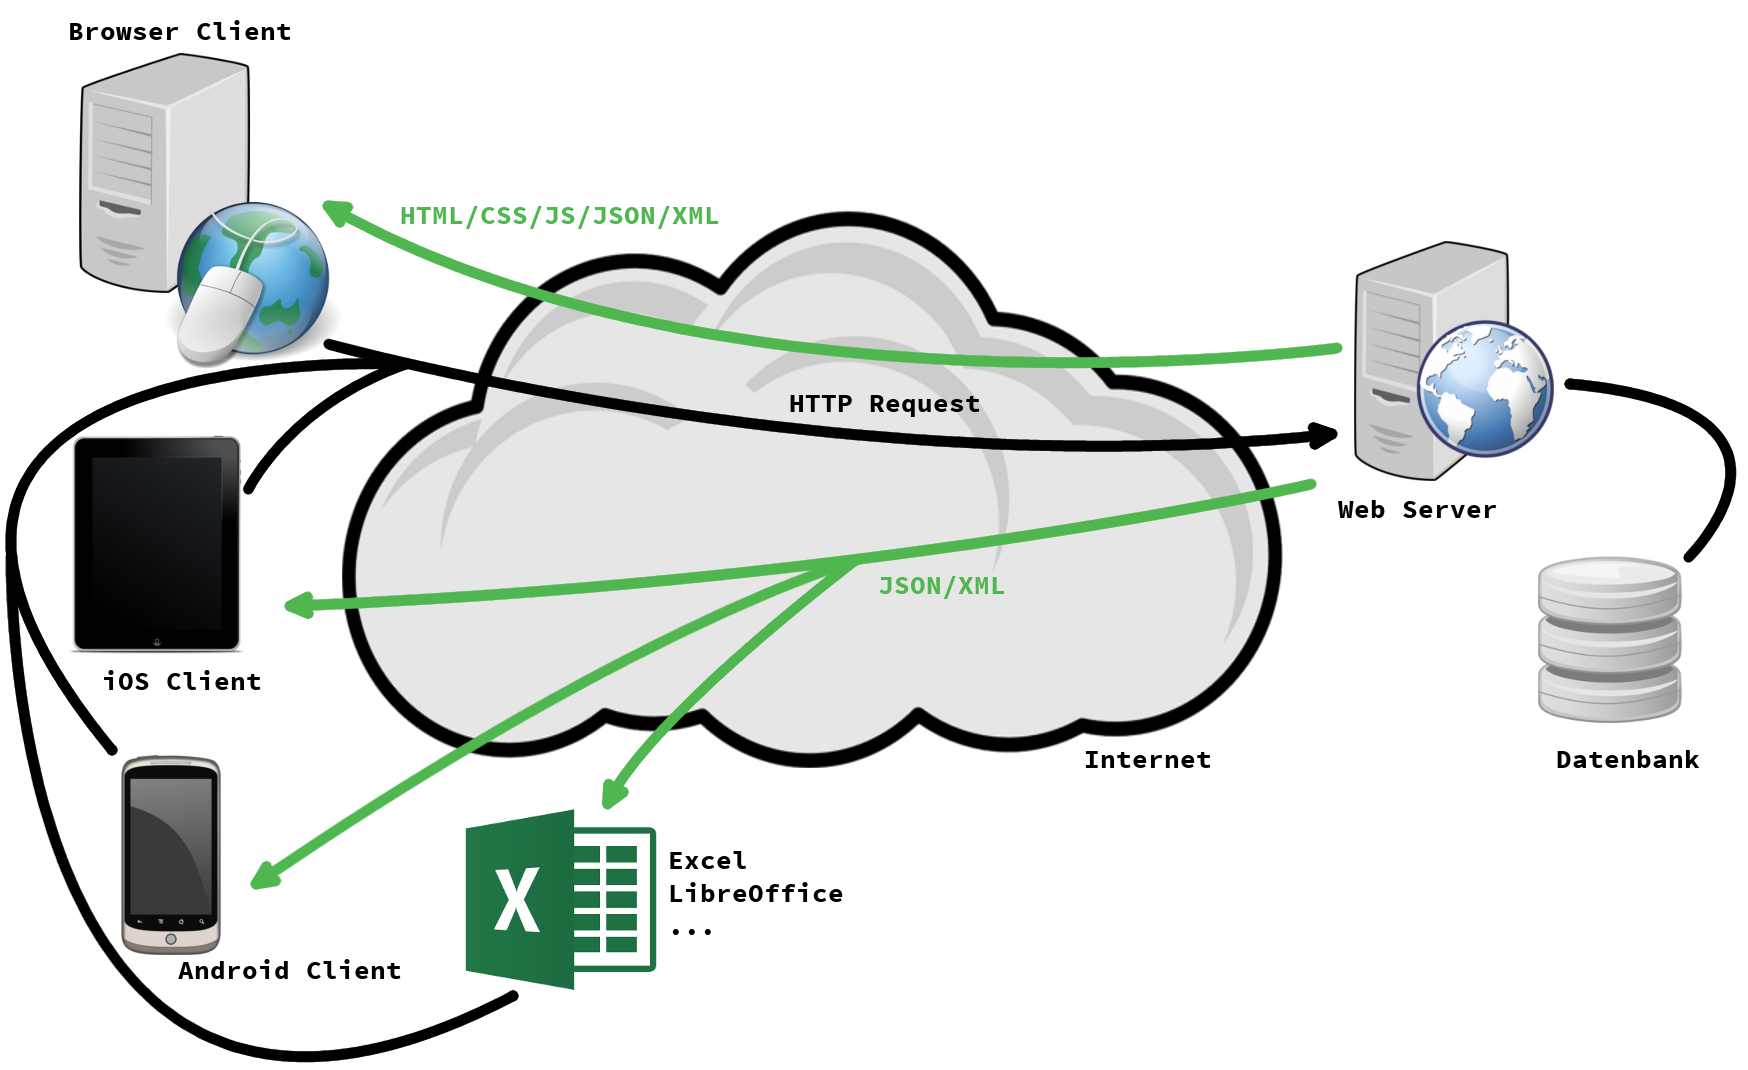
\includegraphics[width=0.6\textwidth]{img/webservice.png}
	\captionsetup{format=hang}
	\caption{Prinzip eines Webservice}
	\small Quelle: \url{https://www.ransoft.at/images/others/webservice.png}
	\label{fig:webservice}
\end{figure}
% !TEX root =  ../theoretisch.tex
\subsection{Representational State Transfer}
\label{sec:grundlagen:rest}
Die Schnittstellenentwicklung ist in der heutigen Webentwicklung allgegenwärtig.
Gerade die bekannten Internetunternehmen wie Google\autocite{MS-GoogleLLC.2020}, Twitter\autocite{MS-TwitterInc..01.03.2020} oder Microsoft\autocite{MS-MicrosoftCorporation.21.05.2018} bieten teilweise dutzende öffentliche Schnittstellen in Form von \acp{API} an.
Allein Google betreut über 100 verschiedene öffentliche \acp{API}\autocite{rf-google-api-alle}.
Durch die Verwendung einer \ac{API} ist es möglich, Software an einer Microservice-Architektur auszurichten und somit die Wartbarkeit und Langlebigkeit zu verbessern.\autocite{rf-fowler2015microservices}

Der wohl bekannteste und derzeit verbreiteste Schnittstellentyp ist \ac{REST}.
\ac{REST} basiert dabei auf dem \ac{REST}-Paradigma, welches von Roy Thomas Fielding in seiner Dissertation\autocite{MS-Fielding.} vorgestellt wurde. Allgemein hat das \ac{REST}-Paradigma sechs Grundprinzipien, die bei der Entwicklung einer \ac{REST}-basierten \ac{API} beachtet werden müssen. 
Aus diesem Grund gilt \ac{REST} auch nicht als Standard, sondern gibt eine grobe Richtung für die Entwicklung von \acp{API} vor.
Im Nachfolgenden werden die sechs Grundprinzipien genauer erläutert:

Das erste Prinzip beruht auf einer Client-Server-Architektur, bei der die Benutzerschnittstelle von der Datenhaltung entkoppelt wird. % ref zum kommenden Kapitel?
Hierdurch soll die Skalierbarkeit und Portabilität der Software verbessert werden.
Als zweites Grundprinzip wird die Zustandslosigkeit angesehen.
Damit ist gemeint, dass alle Anfragen vom Client an den Server stets alle nötigen Informationen beinhalten, die der Server benötigt.
Dabei werden Aktionen bzw. Anfragen isoliert betrachtet, was sowohl das Nachvollziehen dieser erleichtert als auch die Zuverlässigkeit des Systems verbessert.

Der dritte Grundsatz nach \citeauthor{MS-Fielding.} ist der Cache. 
Laut diesem Prinzip sollen die Daten als \enquote{cachable} oder \enquote{not cachable} markiert werden.
Dadurch wird festgelegt, ob Antworten vom Server gespeichert und erneut verwendet werden dürfen, was die Effizienz des Systems erhöht und redundante Anfrage unterbindet.
Das nächste Prinzip bezieht sich auf die Gestaltung der Schnittstellen. 
Diese sollen möglichst einheitlich aufgebaut sein, sodass es dem Nutzer ermöglicht wird, schnell die Struktur der Schnittstellen zu verstehen. 
Dies hilft den Code allgemein zu vereinfachen bzw. Arbeitsschritte nachvollziehbar zu gestalten.

Das fünfte Prinzip nach \citeauthor{MS-Fielding.} ist die hierarchische Strukturierung des Gesamtsystems in verschiedene Schichten. 
Die Schichten sollen ermöglichen, dass jede Komponente nur die direkten Nachbarkomponenten kennt und keine Daten oder Funktionalitäten aus anderen Schichten auslesen und verwenden kann.
Dadurch können Komponenten von der Außenwelt abgekapselt bzw. isoliert werden.
Weiterhin kann dadurch eine bessere Lastverteilung über verschiedene Netzwerke ermöglicht werden.
Der letzte Grundbaustein des \ac{REST}-Paradigmas sind nachladbare Funktionalitäten.
Dieses Prinzip ist optional und bezieht sich darauf, dass die Client-Funktionalität durch das Herunterladen von ausführbarem Code erweitert werden kann. 

Neben den gerade genannten sechs Prinzipien beschreibt \citeauthor{MS-Fielding.} in seiner Dissertation noch die zu \ac{REST} gehörigen Datenelemente. 
Dabei spielt das Datenelement namens Ressource eine zentrale Rolle.
Eine Ressource verkörpert in \ac{REST} eine Abstraktion der Information in jeglicher Form.
Es ist dabei egal, ob es sich um ein Bild, ein Dokument oder um komplexe Sachverhalte handelt. 
Wichtig ist jedoch, dass das Ziel einer Hypertext-Referenz mit der Definition einer Ressource übereinstimmt.
Ressourcen selbst können entweder statisch oder dynamisch sein.
Diese Unterscheidung ermöglicht, dass eine statische Ressource jederzeit denselben Zielwert zurückliefert, während eine nicht statische Ressource verwendet werden kann, um beispielsweise die aktuellste Version des Wertes zurück zu geben.\autocite[Vgl.][S. 86-90]{MS-Fielding.}$^,$\autocite{rf-richardson2013restful}

Da \ac{REST} selbst kein Standard, sondern ein Rahmenwerk für die Architektur von Schnittstellen darstellt gibt es verschiedene Formen, wie eine Umsetzung erfolgen kann. 
Oftmals wird für die Umsetzung von \ac{REST}-basierten \acp{API} das \ac{HTTP} verwendet.
\ac{HTTP} bringt viele Eigenschaften mit, die das \ac{REST}-Paradigma voraussetzt und stellt deshalb eine denkbar perfekte Grundlage für die Implementierung von \ac{REST}-\acp{API} dar. 
Durch die in \ac{HTTP} implementierten Methoden wie \emph{GET}, \emph{POST}, \emph{PUT} und \emph{DELETE} ist es möglich, die im Paradigma beschriebenen Ressourcen zu verwalten.
Die Übertragung der Nutzdaten erfolgt dabei meist im \acs{JSON}- oder \acs{XML}-Format.\autocite[Vgl.][S. 97]{MS-Tilkov.2015} 


\section{\acf{JSON}}
\label{sec:json}

Für den Datenaustausch zwischen Front- und Back-End wird mit der \acf{JSON} realisiert.
Grund ist, dass hier rein die Nutzdaten transferiert werden.
Ferner gestaltet sich das Auslesen und Generieren der \acs{JSON}-Dateien als recht \enquote{einfach}. \\
Ein Array bzw. eine Liste wird in \acs{JSON} mit [ ] dargestellt.
Objekte werden mit \{ \} dargestellt.
Jedes Attribut und jede Zeichenkette wird in \acs{JSON} in Anführungszeichen gesetzt (siehe Quelltext \vref{lst:example_movie}).

\begin{lstlisting}[language=json, caption={Beispiel eines Films im \acs{JSON}-Format}, label={lst:example_movie}]
{"movie": {
	"id": 1,
	"title": "Kampf der Titanen",
	"duration": 120,
	"hall": {
		"id": 1,
		"name": "Kino 1",
		"seats": [{"seat": {"id": 1, ...}}]
	},
	"shows": [{"show": {"id": 1, ...}}]
 }
}
\end{lstlisting}

\section{Generieren der \acf{JSON}}
\label{sec:json_generieren}

Java ist eine objektorientierte Sprache.
Alle Klassen sind dementsprechend als Objekte hinterlegt.
Durch die Implementierung eines sog. Object-Mappers wie dem Jackson-Mapper\footnote{\url{https://github.com/FasterXML/jackson}}
ist es möglich die zuvor erstellten Objekte in eine \acs{JSON}-Datei zu überführen.
Er erkennt automatisch, ob es sich um ein Objekt, ein Attribut oder eine Liste handelt.
Der Entwickler ruft lediglich die Methode \jinline |writeValueAsString(Object-to-JSON)|, die ein Objekt als Übergabeparameter erwartet auf. \\
Das Auslesen eines \acs{JSON}-Strings wird mit der Methode \texttt{readValue(json, javaClass)} ausgeführt.
Diese erwartet als Übergabeparameter ein \acs{JSON}, sowie die Java-Klasse des Objekts, in es gewandelt werden soll z.B. \jinline |Show.class|.
Der Vorteil dieser Methode ist, dass hier die Java-Klasse angegeben wird, also das Objekt, in das der \acs{JSON}-String konvertiert werden soll.

Der Jackson-Mapper wird in diesem Projekt über eine Dependency zu einem Maven-Projekt hinzugefügt und kann anschließend verwendet werden (siehe Quelltext \ref{lst:Einbindung_ObjektMapper}) %TODO varioref

\begin{lstlisting}[language=XML, caption={Einbindung des Objekt-Mappers in die pom.xml}, label={lst:Einbindung_ObjektMapper}]
<dependency>
	<groupId>com.fasterxml.jackson.core</groupId>
	<artifactId>jackson-databind</artifactId>
	<version>2.9.4</version>
</dependency>
\end{lstlisting}

\begin{lstlisting}[style=lstJava, caption={Ausschnitt aus der selbst erstellten Klasse JSONConverter}]
public static String toJSON ( Object object ) throws JsonProcessingException
{
	String str = "";
	ObjectMapper om = new ObjectMapper();
	om.getSerializerProvider().setNullKeySerializer(nullKeySerializer);
	str = om.writeValueAsString(object);
	return str;
}

public static Object fromJSON ( String json, Class<?> javaClass ) throws IOException
{
	ObjectMapper om = new ObjectMapper();
	om.configure(DeserializationFeature.FAIL_ON_UNKNOWN_PROPERTIES, false);
	Object obj = om.readValue(json, javaClass);
	return obj;
}
\end{lstlisting}

% !TEX root =  master.tex
\section{\acf{DTO}}
\label{sec:dto}

\subsection{Begriff \acf{DTO}}
\label{ssec:Was_ist_dto}

Der Begriff \ac{DTO} ist ein Entwurfsmuster, welches aus dem Bereich der Softwareentwicklung stammt.
Es wird genutzt, um mehrere Objekte in einem Programmaufruf zusammenzufassen, weshalb es Anwendung in verteilten Systemen findet.\footnote{\url{https://www.georgbeier.de/tutorials-java-und-mehr/java8-spring-groovy-vaadin/svg-architecture/data-transfer-objects/}}

Ein \ac{DTO} entspricht eigentlich dem \ac{POJO}.
Es hat nahezu die selben Attribute, kann aber nach Belieben verändert werden.
So kann man sich mittels des \ac{DTO} nur einige Attribute anzeigen lassen und die Entität bleibt unberührt.

Die \acsp{DTO} werden in diesem Projekt dazu genutzt, um die Daten aus der Datenhaltungsschicht der Drei-Schichten-Architektur in die Logik- bzw. Fachkonzeptschicht zu transferieren, denn eine Entität verlässt niemals die Datenhaltungsschicht.
Von dort aus werden sie als \acs{JSON} an die Benutzerschicht weitergeleitet.

\subsection{Umwandlung der Entität zu und von einem \acf{DTO}}
\label{ssec:umwandlung_dto}

Wie bereits beschrieben kommen in diesem Projekt \acp{DTO} zum Einsatz.
Um eine Umwandlung zu realisieren wurden zwei Java-Klassen implementiert: \jinline|EntityToToHelper| und \jinline|ToToEntityHelper|. 

Die Klasse \jinline|EntityToToHelper| ist dafür verantwortlich, die zuvor über das \acs{DAO} angefragte Entität mit all ihren Attributen in ein \acs{DTO} umzuwandeln, sodass es transferierbar ist. \\
Ein Beispiel für die Umwandlung von einer Entität in ein \acs{DTO} befindet sich im Anhang \vref{lst:EntityToToHelper_movie}. \\

Die Klasse \jinline|ToToEntityHelper| ist dafür verantwortlich das zuvor über das \acs{JSON} übermittelte \acs{DTO} mit all seinen Attributen in ein Entität umzuwandeln, sodass es persistier-, änder- oder löschbar ist.\\
Ein Beispiel für die Umwandlung von einem \acs{DTO} in eine Entität befindet sich im Anhang \vref{lst:ToToEntityHelper_movie}.

% !TEX root =  master.tex
\section{Sitzplatzauswahl und Blockierungen}
\authorsection{\authorNL}

Beim Reservierungsvorgang ist es essentiell, dass ein Sitzplatz nicht mehrfach reserviert wird.

Hier ein einfaches Beispiel:
Benutzer A besucht die Seite, wählt einen Film und eine Vorstellung aus.
Die Saalübersicht wird geladen, wobei Sitzplätze, die bereits reserviert sind, optisch hervorgehoben sind und nicht mehr ausgewählt werden können.
Etwa zur gleichen Zeit besucht Benutzer B die Seite.
Er wählt die selbe Vorstellung, sieht die gleiche Saalübersicht und wählt einen Platz aus: Reihe 4, Platz 2.
Benutzer B folgt daraufhin den weiteren Schritten, bezahlt seinen Sitzplatz und erhält eine Bestätigung, dass Reihe 4, Platz 2 erfolgreich von ihm gebucht wurde.
Auch Benutzer A hat Reihe 4, Platz 2 ausgewählt.
Zu dem Zeitpunkt als Benutzer A den Saalplan geladen hat, war die Reservierung von Benutzer B noch nicht abgeschlossen, sodass der Platz frei war.
Auch Benutzer A möchte nun das Ticket bezahlen, muss aber eine Fehlermeldung erhalten, damit das Ticket für Reihe 4, Platz 2 nicht doppelt verkauft wird.

Spätestens bei der verbindlichen Reservierung und der normalerweise folgenden Bestätigung muss eine Fehlermeldung erscheinen, wenn der Platz bereits belegt ist.
Im Idealfall wird der Nutzer aber schon früher benachrichtigt, wenn er einen Platz ausgewählt hat, der in der Zwischenzeit von einem anderen Benutzer reserviert wurde.

Der Fall, dass ein Platz durch einen anderen Benutzer reserviert wird, ist mit gewisser Wahrscheinlichkeit vorhersehbar.
Wählt ein Benutzer im Saalplan ein paar Plätze aus, so wird er vermutlich in den nächsten paar Minuten mit der Bezahlung fortfahren und die Plätze für sich reservieren.
In dem Moment, wo ein Benutzer einen Sitzplatz also nur auswählt, kann diese Information bereits in der Datenbank gespeichert werden.
Der Sitzplatz wird für diesen Benutzer zwar nicht reserviert, aber für einen kurzen Zeitraum vorgemerkt.
Will nun jemand einen Platz auf dem Saalplan auswählen, teilt er dies über die \acs{API} dem Back-End mit.
Nun gibt es mehrere mögliche Ergebnisse:
\begin{enumerate}
\item Der ausgewählte Sitzplatz ist bereits reserviert.
\item Der ausgewählte Sitzplatz ist bereits für einen anderen Benutzer vorgemerkt, könnte also in einigen Minuten wieder frei werden.
\item Der Sitzplatz ist weder reserviert, noch vorgemerkt.
Er wurde nun erfolgreich für den aktuellen Benutzer vorgemerkt.
\end{enumerate}

Dies kann nun dazu führen, dass ein Benutzer einen freien Saalplan angezeigt bekommt und beim Anklicken eines Platzes dieser nun nicht mehr als \enquote{frei}, sondern als \enquote{durch einen anderen Nutzer belegt} angezeigt wird.

Die zu der Reservierung zugehörigen Operationen auf der Datenbank müssen atomar ausgeführt werden, sodass die Reservierung entweder erfolgreich war oder eine Fehlermeldung den Benutzer informiert, dass die Reservierung fehlgeschlagen ist.

Alle Sicherheitsprüfungen müssen im Back-End ausgeführt werden.
Natürlich können auch einzelne Prüfungen im Front-End implementiert werden, diese helfen allerdings nur einem normalen Benutzer den Vorgang zu erleichtern.
Eine Absicherung bieten derartige Prüfung im Front-End nicht, da der clientseitig ausgeführte Quellcode logischerweise vom Client verändert werden kann und jeder Angreifer eine manipulierte Anfrage mit selbst gewählten Parametern an die \acs{API} schicken kann.
\section{Reservieren}
\label{sec:reservieren}

\subsection{Herausforderung}
\label{ssec:herausforderung_reservieren}

Eine weitere Herausforderung bestand darin, das Reservieren eines Sitzes im Back-End zu realisieren.
Hierfür mussten ebenso verschiedene Aspekte betrachtet werden.

\begin{enumerate}
	\label{enum:reservieren}
	\item \label{itm:zeitpunkt_reservieren}Das Reservieren darf nur, wie das Blocken, bis zu einem bestimmten Zeitpunkt möglich sein.
	\item \label{itm:geblockt_durch_benutzer} Falls der Sitzplatz durch den selben Benutzer geblockt wurde, darf dieser diesen buchen.
	Andernfalls darf es keine erfolgreiche Reservierung geben.
	\item \label{itm:mehr_eine_vorstellung_reservieren}Eine Mehrfachvergabe des selben Sitzplatzes für eine Vorstellung muss wie beim Blocken ausgeschlossen sein (vgl. Herausforderung \ref{enum:blocken} Punkt \ref{itm:mehr_eine_vorstellung}).
	\item \label{itm:mehr_mehrere_vorstellungen_reservieren}Die Belegung eines Sitzes für verschiedene Vorstellungen muss gewährleistet sein.
	\item \label{itm:ticket_reservieren} Der Sitzplatz darf nur reserviert werden, wenn es für ihn noch kein Ticket gibt und er derzeit auch nicht blockiert ist.
	\item \label{itm:front_end_reservieren} Eine Information mit den erfolgreich reservierten Sitzen muss an das Front-End gesendet werden.
	\item \label{itm:zeit_reservieren} Der Zeitpunkt der Reservierung darf durch das Front-End nicht manipulierbar sein.
\end{enumerate}

\subsection{Lösungsansatz}
\label{ssec:loesung_reservieren}

Um die geforderten o.g. Punkte umzusetzen, werden in der \acs{REST}-Schnittstelle \\\jinline |reservation/book| mehrere Überprüfungen durchgeführt.

\subsubsection*{Punkt \ref{itm:zeitpunkt_reservieren} -- Zeitpunkt}
\label{ssssec:Zeitpunkt_reservieren}
Siehe \nameref{ssec:loesung_blocken} \nameref{ssssec:Zeitpunkt} auf Seite \pageref{ssssec:Zeitpunkt}.

\subsubsection*{Punkt \ref{itm:geblockt_durch_benutzer} -- Geblockt durch Benutzer, Punkt \ref{itm:mehr_eine_vorstellung_reservieren}, \ref{itm:mehr_mehrere_vorstellungen_reservieren} -- Mehrfachvergabe, Punkt \ref{itm:ticket_reservieren} -- Reservieren}
\label{ssssec:geblockt_durch_benutzer}
Um einem Benutzer das Reservieren des möglicherweise geblockten Sitzplatzes für eine Vorstellung zu gewährleisten, wurde, wie bereits erwähnt, sich dazu entschlossen einen Sessiontoken als Identifikator mitzugeben.
Da dieser vom Front-End erzeugt wird, reicht dieses den Sessiontoken beim Reservierungsvorgang im \acs{JSON} mit.
Da der Sessiontoken auch hier nach erfolgreicher Buchung nicht übermittelt werden soll, gibt es auch für diesen Anwendungsfall zwei \acp{DTO}, die wie im \nameref{ssec:loesung_blocken} Blocken in \nameref{ssssec:Bezeichner} auf Seite \pageref{ssssec:Bezeichner} auch die \acs{JSON}-Annotation, für das Schreiben bzw. Nichtschreiben des Sessiontokens, besitzen (\textit{BookingToWithSessiontoken} und \textit{BookingTo}). 

Auch hier erfolgt durch eine ausgelagerte Methode \jinline |checkIfSeatsAreBookable| die Überprüfung, ob
\begin{enumerate}
	\item es bereits ein Ticket für den zu buchenden Sitzplatz gibt.
	\item der Sitzplatz bereits geblockt ist.
	\begin{enumerate}
		\item Wenn ja, passt der Sessiontoken der aktuellen Anfrage zu diesem? Dann darf die Buchung erfolgen.
		\item Falls nicht, darf die Reservierung nicht erfolgen.
	\end{enumerate}
\end{enumerate}

War dieser Methoden-Aufruf erfolgreich, wird eine weitere Methode aufgerufen, die ein Reservierungs-\acs{DTO} als Rückgabewert hat (\jinline |createReservationForSeats|). \\
Dieses ist mit dem aktuellen Datum und der aktuellen Uhrzeit sowie einer Liste mit Ticket-\acp{DTO} versehen.
Dem Ticket-\acs{DTO} wird der aktuelle Sitzplatz zugeteilt.
Ferner wird in jedem Ticket-\acs{DTO} individuell das Attribut \jinline |isReducedPrice| gesetzt, welches zuvor durch das Front-End zu dem jeweiligen Sitzplatz über das \acs{JSON} mitgeteilt wurde.
Durch dieses Setzen des Attributs hat man im Nachhinein die Möglichkeit, die korrekte Preisberechnung zu verifizieren.

Die Implementierung, ob die ausgewählten Sitzplätze verfügbar sind, befindet sich im Anhang \vref{lst:Angang_Prüfung_ob_Reservierung_möglich}.
Die Implementierung für das Erstellen des Reservierungs-\acp{DTO} befindet sich im Anhang \vref{lst:Anhang_Erstellen_Reservierung}.

\subsubsection*{Punkt \ref{itm:front_end_reservieren} -- Erfolgreich}
\label{ssssec:front_end_reservieren}
Wurde der Reservierungsvorgang erfolgreich durchgeführt, erhält das Front-End das Reservierungs-\acs{DTO} als \acs{JSON} wie in \nameref{ssec:loesung_blocken} im \nameref{ssssec:erfolgreich_blocken} auf Seite \pageref{ssssec:erfolgreich_blocken} beschrieben, zur Auswertung zurück (vgl. Herausforderungen Punkt \vref{itm:front_end_reservieren}).
Diese wertet das \acs{JSON} aus und generiert daraus einen \acs{QR-Code}, der im Browser angezeigt wird.
Ein Beispiel für die Umsetzung seitens des Front-Ends befindet sich in Kapitel \vref{fig:vorstellung04}.
%Dieses hat wie zuvor beschrieben das Attribut \jinline |sessiontoken| nicht gesetzt.


% !TEX root =  master.tex
\chapter{Front-End}
\chapterauthor{\authorNL}
\section{Technologien}
\label{sec:technologien}

Für das hier erstellte Kinoreservierungsprogramm wurde die Verwendung von Java\footnote{\url{https://java.com/de/download/} -- Version 8.0.141 verwendet} für das Back-End vorgegeben. 

Als Java-\acs{IDE} kommt Eclipse\footnote{\url{https://www.eclipse.org/} -- Version: Photon Release (4.8.0)} zum Einsatz, da es aus vorangegangenen Vorlesungen bekannt ist.
Für die Kommunikation zwischen den einzelnen Schichten der Drei-Schichten-Architektur kommen \acs{REST}ful-Webservices in Verbindung mit Jersey\footnote{\url{https://jersey.github.io/} -- Version 1.19.4} sowie \acp{DTO} zum Einsatz (Kapitel \vref{sec:dto}), die zwischen den einzelnen Schichten transferiert werden.

Um eine Datenhaltung und den Austausch von Informationen zu gewährleisten, wurde sich in dieser Arbeit für eine Postgres Datenbank entschieden.
Der Zugriff auf die Datenbank erfolgt mittels der \ac{JPA} in Verbindung mit EclipseLink (Kapitel \vref{ssec:jpa}).
% !TEX root =  master.tex
\section{Startseite mit Filmübersicht}

Auf der Startseite sieht der Benutzer direkt das Kinoprogramm.
Ganz oben befindet sich ein \enquote{Karussell} mit den aktuellen Blockbustern.
Dieses basiert auf einer Vorlage für Bootstrap, passt sich durch eine eigene Implementierung automatisch an die Bildschirmgröße und auch an die Größe des aktuell angezeigten Bildes an, sodass die Inhalte des Karussells möglichst groß, aber dennoch korrekt dargestellt werden.
Direkt darunter folgt dann die Liste mit den Filmen.

\begin{figure}[ht]
	\centering
	\subfloat[Desktop-Computer]{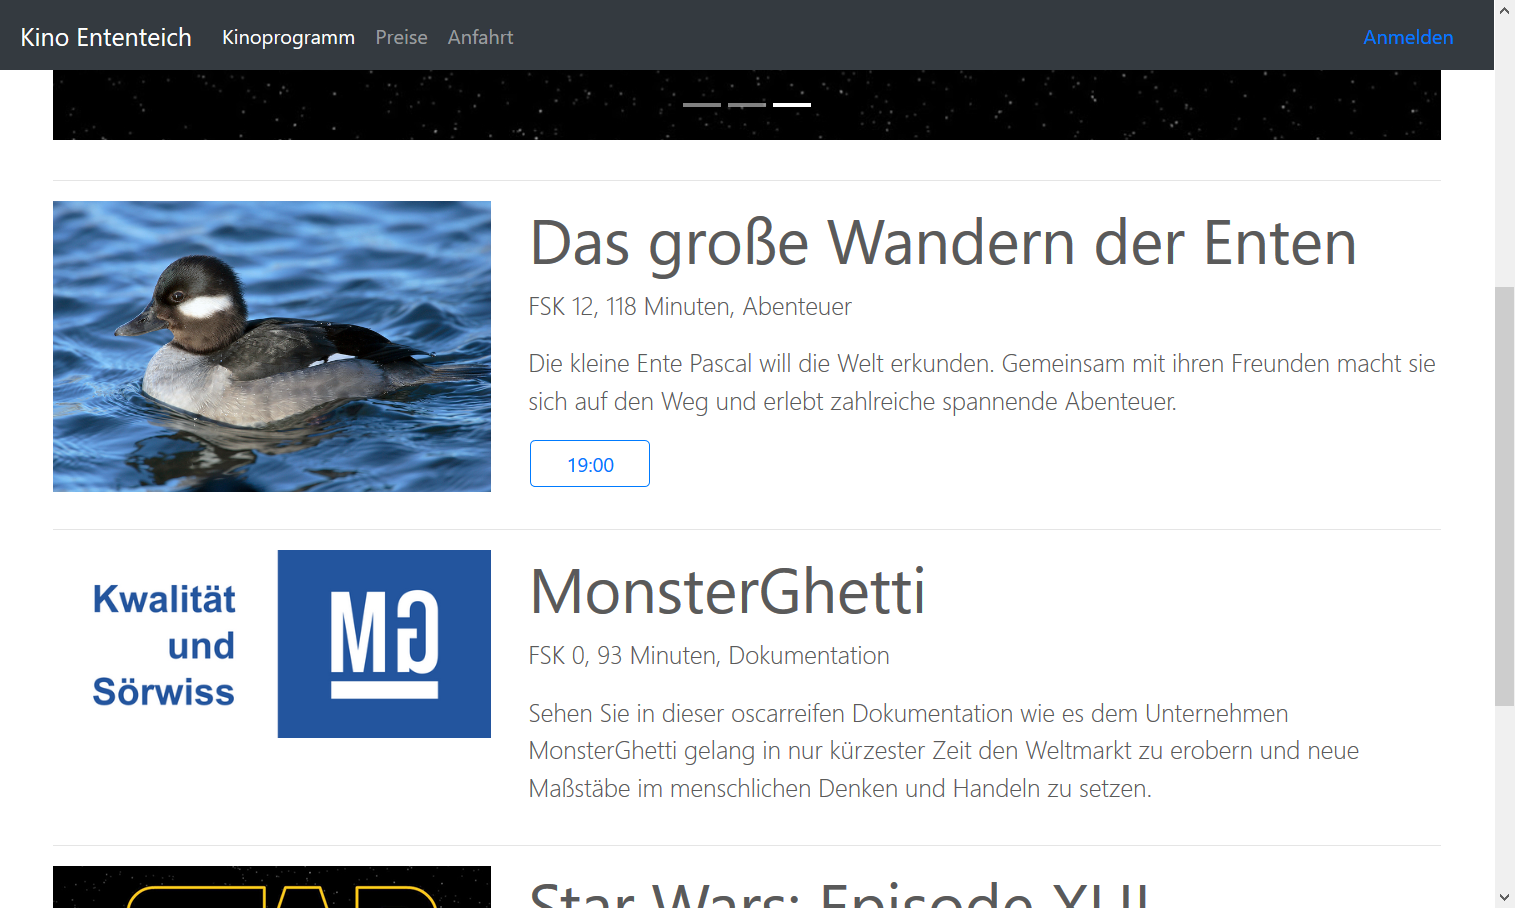
\includegraphics[height=0.28\textheight]{img/screenshots/startseite01}
	\label{fig:startseite01}}
	\hfill
	\subfloat[Mobiles Gerät]{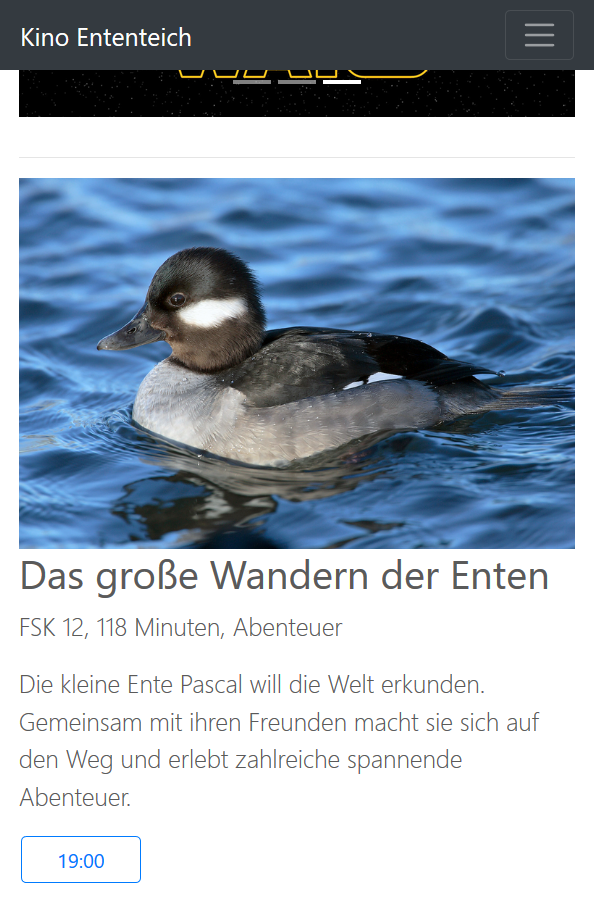
\includegraphics[height=0.28\textheight]{img/screenshots/startseite02}
	\label{fig:startseite02}}
	\caption{Filmübersicht auf der Startseite}
\end{figure}

Dabei ist zu jedem Film neben dem Titel auch noch ein Bild zu sehen.
Allgemeine Informationen zum Film sowie eine Beschreibung ermöglichen es dem Benutzer, sich einen schnellen ersten Eindruck von dem jeweiligen Film zu verschaffen.
Durch Anklicken des Filmtitels oder des Bildes gelangt man zu den Vorstellungen und weiteren Details.
Um Benutzern einen Klick zu ersparen, sieht man sogar direkt die heutigen Vorstellungen und kann gegebenenfalls sofort zu diesen Vorstellungen springen und Sitzplätze auswählen.

Je nach Größe des Bildschirms, wir der Inhalt entsprechend angezeigt.
Bei breiten Bildschirmen, wie es meist bei Desktop-Computern und Laptops der Fall ist, ist genügend Platz, um Bild und Text nebeneinander anzuzeigen.
Bei Smartphones hingegen, wäre das Bild so kaum erkennbar und es würden nicht viele Wörter in eine Zeile passen.
Dementsprechend werden bei solchen Bildschirmen Bild und Text untereinander angezeigt.
All diese Anpassungen werden durch \acs{CSS}-Anweisungen veranlasst, inhaltlich gibt es keine Unterschiede.
% !TEX root =  master.tex
\section{Anbindung an das Back-End}
\label{sec:anbindung_backend}

Um die Daten aus der Datenbank bzw. dem Back-End anzuzeigen, werden diese durch einen oder mehrere \acs{AJAX}-Aufrufe nachgeladen.
Beim Laden der Startseite wird die Funktion \textit{loadMovies()} aufgerufen.
Diese wiederum ist nur für die Zuordnung von einem Pfad bzw. einer \acs{URI} zu einer Funktion, die das Ergebnis verarbeitet, da.
Sie würde auch \acs{URL}-Parameter auslesen und in den Aufruf mit einarbeiten, dies ist aber auf der Startseite noch nicht notwendig.

\begin{lstlisting}[language=JavaScript, caption={\acs{AJAX}-Aufruf, um alle Filme zu erhalten}, label={lst:ajax_all_movies}]
const URL_SERVER = "http://localhost:8080/cinema-system";
const PATH_ALL_MOVIES = "/movie/getAllMovies";

function getData (path, func) {
	$.ajax({
		type: "GET",
		url: URL_SERVER + path,
		success: (data) => func(data)
	});
}

function loadMovies () {
	getData(PATH_ALL_MOVIES, displayMovies);
}

function displayMovies (movies) {
	...
}
\end{lstlisting}

Der \acs{AJAX}-Aufruf wird asynchron durchgeführt.
Das Ergebnis wird, wenn es beim Client angekommen ist, an die Funktion \textit{displayMovies()} weitergegeben, die nun dafür zuständig ist, die Daten entsprechend anzuzeigen.

Die Funktion \textit{getData()} dient hier als Schnittstelle zum Back-End und wird im Grunde an allen Stellen genutzt, bei denen Daten vom Back-End abgefragt werden.
Als Parameter erhält sie den Pfad, der vom Server nachgefragt werden soll, sowie eine Referenz auf eine Funktion, die das Ergebnis verarbeitet.

Wenn der Aufruf an das Back-End noch einen oder mehrere Parameter enthält, wie zum Beispiel beim Laden eines einzelnen Films mit seinen Details und Vorstellungen, so wird dieser Parameter in der zugehörigen \textit{load}-Funktion hinzugefügt.

\begin{lstlisting}[language=JavaScript, caption={Laden der Filmdetails nach Auslesen der \acs{URL}-Parameter}, label={lst:load_movie_and_shows}]
const PATH_MOVIE = "/movie/{movieID}";

function loadMovieAndShows () {
	var movieID = urlparameters.get("id");
	if (movieID == null) {
		window.location.href = "./index.html";
	}
	else {
		getData(PATH_MOVIE.replace("{movieID}", movieID), displayMovieAndShows);
	}
}

function displayMovieAndShows (movie) {
	...
}
\end{lstlisting}

Wie in Quelltext \vref{lst:load_movie_and_shows} erkennbar ist, wird der Platzhalter \textit{movieID} einfach durch den aus der \acs{URL} ausgelesenen Wert ersetzt.
Danach wird genauso wie in Quelltext \vref{lst:ajax_all_movies} die Anfrage an das Back-End gestellt und das Ergebnis in einer weiteren Funktion verarbeitet und angezeigt.
% !TEX root =  master.tex
\section{Filmdetails und Vorstellungsauswahl}

Nachdem die Daten wie in Quelltext \ref{lst:load_movie_and_shows} geladen wurden, muss nun das \acs{DOM} entsprechend verändert werden.
Die statische \acs{HTML}-Seite ist dabei auf das Wesentliche reduziert und enthält neben der Menüleiste und der Fußzeile folgenden Teil:

\begin{lstlisting}[style=lstHTML, caption={\acs{HTML}-Seite für Filmdetails}, label={lst:html_movie_and_shows}]
<div class="container" id="movie">
	<!-- Informationen zum Film werden hier eingefügt -->
	<table class="table" id="shows">
		<tr>
			<th>Tag</th>
			<th>Vorführungen</th>
		</tr>
		<!-- die einzelnen Vorstellungen werden hier eingefügt -->
	</table>
	<!-- Bewertungen werden hier eingefügt -->
</div>
\end{lstlisting}

An den gekennzeichneten Stellen wird später der Inhalt, der aus dem Back-End geladen wurde, eingefügt.
Dafür gibt es kleinere Vorlagen mit Platzhaltern.

\begin{lstlisting}[style=lstHTML, caption={\acs{HTML}-Vorlage mit Platzhaltern für Filmdetails}, label={lst:html_template_movie_detail}]
<div class="row featurette">
	<div class="col-12 col-sm-4">
		<img class="featurette-image img-fluid mx-auto" src="./img/`\textcolor{red}{\{movieID\}}`.jpg" alt="`\textcolor{red}{\{movieTitle\}}`" width="100%">
	</div>
	<div class="col-12 col-sm-8">
		<h2 class="featurette-heading">`\textcolor{red}{\{movieTitle\}}`</h2>
		<p>FSK `\textcolor{red}{\{movieFSK\}}`, `\textcolor{red}{\{movieDuration\}}` Minuten, `\textcolor{red}{\{movieGenres\}}`</p>
		<p class="rating-`\textcolor{red}{\{movieRatingRounded\}}`">`\textcolor{red}{\{movieRating\}}`</p>
	</div>
</div>

<div class="row featurette">
	<div class="col-12">
		<p>`\textcolor{red}{\{movieDescription\}}`</p>
	</div>
</div>
\end{lstlisting}

%Dabei wir davon ausgegangen, dass die Bilder für die Filme als statische Inhalt unter einem festen Namen gespeichert sind, z.B. \textit{1.jpg}.

In JavaScript wird diese Vorlage dann mit Inhalten befüllt.
Nachdem die Daten in der Funktion \textit{displayMovieAndShows()} ein wenig verarbeitet wurden, können sie mit JavaScript bzw. jQuery in die Vorlage und danach ins \acs{DOM} eingefügt werden.

\begin{lstlisting}[language=JavaScript, caption={Einfügen der Filmdetails ins \acs{DOM} mit jQuery}, label={lst:js_write_movie_detail_to_dom}]
$("#movie").prepend(templateMovieDetail
	.replace("{movieID}", movie.id)
	.replace(/\{movieTitle\}/g, movie.name)
	.replace("{movieFSK}", movie.fsk)
	.replace("{movieDuration}", movie.duration)
	.replace("{movieGenres}", genres)
	.replace("{movieRatingRounded}", Math.max(0, Math.min(5, Math.round(rating))))
	.replace("{movieRating}", (movie.ratings.length > 0 ? rating.toFixed(1).replace(".",",") : "") + " (" + movie.ratings.length + " Bewertung" + (movie.ratings.length == 1 ? "" : "en") + ")")
	.replace("{movieDescription}", movie.description)
);
\end{lstlisting}

Genauso wie die Filmdetails werden auch die Vorstellungen und die Bewertungen ins \acs{DOM} eingefügt.
Ausschnitte von der vollständig mit Daten befüllten Seite mit allen Details zu einem Film finden sich in Anhang \vref{sec:screenshots_frontend}.

Zusammenfassend heißt das, dass zuerst einmal die statische und weitestgehend leere \acs{HTML}-Seite geladen wird.
Diese wiederum importiert eine JavaScript-Datei, welche beim Laden der Seite eine Anfrage an das Back-End stellt.
Sobald der Server antwortet, wird die Antwort entsprechend verarbeitet und in JavaScript in kleinere Vorlagen eingesetzt.
Die mit Inhalten befüllten Vorlagen werden dann mit jQuery ins \acs{DOM} eingefügt, sodass die \acs{HTML}-Seite die gewünschten Inhalte darstellt.
Dies passiert im Idealfall so schnell, dass es für den Benutzer wirkt, als hätte er die Seite \enquote{ganz normal} geladen.

Damit dies reibungslos funktioniert, ist es essentiell, dass sich die Kommunikation mit dem Server auf ein Minimum beschränkt und keine nicht benötigten oder redundanten Daten transferiert werden.
So ist es zum Beispiel schlecht für die Performance, wenn man im Front-End lediglich eine Liste mit allen Filmen sehen will, aber vom Back-End zu jedem Film alle Vorstellungen mit allen Sitzplätzen erhält.
Genauso muss natürlich auch die Verarbeitung im Front-End effizient erfolgen.
% !TEX root =  master.tex
\section{Implementierung des Saalplans}

\subsection{Darstellung des Kinosaals}

Eine zentrale Aufgabe im Front-End war es, den Kinosaal mit den Sitzen anzuzeigen und dem Benutzer zu ermöglichen, Plätze auszuwählen.

Dies lässt sich mit einfachen Mitteln auch in \acs{HTML} umsetzen, z.B. mit \textit{div}-Elementen, bei denen man Größe und Farbe festlegt.
Mit JavaScript wird dann implementiert, was passiert wenn ein Sitzplatz angeklickt wird.

\begin{figure}[ht]
	\centering
	\subfloat{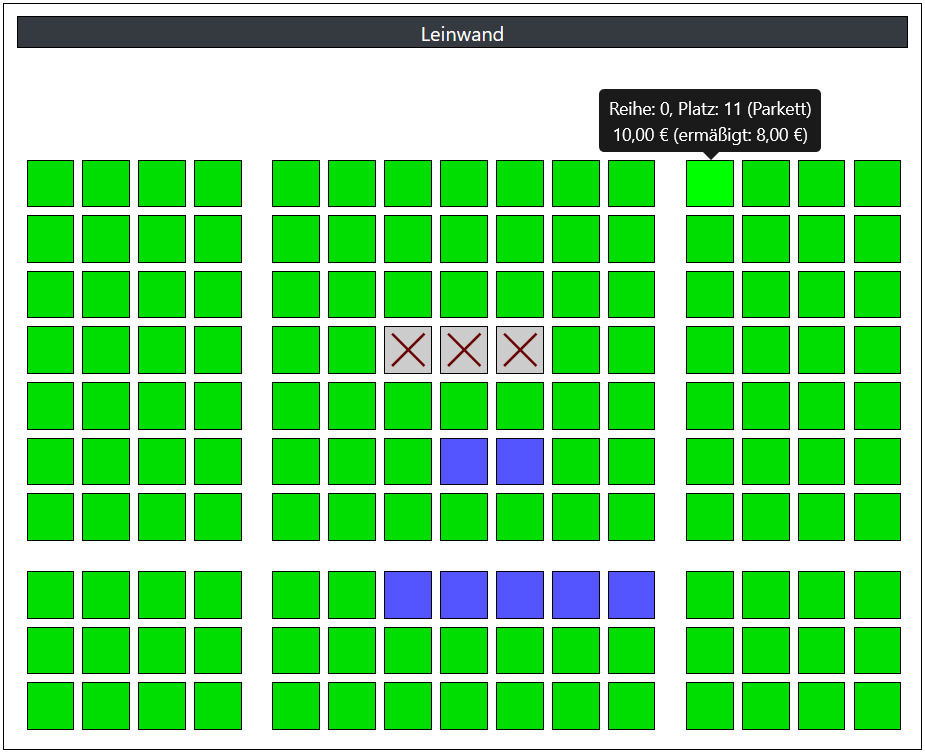
\includegraphics[height=0.295\textheight]{img/screenshots/saalplan01}}
	\hfill
	\subfloat{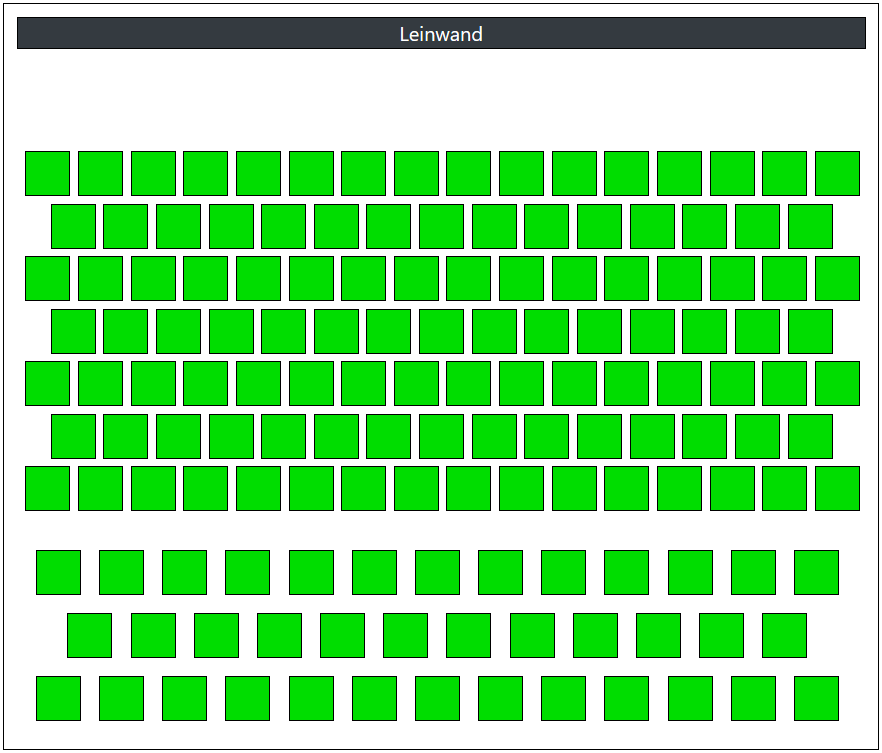
\includegraphics[height=0.295\textheight]{img/screenshots/saalplan03}}

	\caption{Saalpläne}
	\label{fig:saalplan}
\end{figure}

In Abbildung \vref{fig:saalplan} kann man sehen, wie der Kinosaal im Browser dargestellt wird.
Eine Box außen bildet die Umrandung und stellt den Saal dar.
Darin befindet sich eine zweite farblich hervorgehobene Box, die die Leinwand abbildet, damit die Benutzer wissen, wo im Kinosaal vorne und hinten ist, und sie somit ihre Entscheidung, wo sie sitzen möchten, treffen können.
Darunter finden sich dann die Sitzplätze.

Die Sitzplätze sind dabei farblich gekennzeichnet, um anzuzeigen, ob ein Sitzplatz frei oder belegt ist.
Belegte Sitze sind einerseits grau, andererseits auch noch mit einem Kreuz versehen, um Menschen, die in ihrer Farbwahrnehmung eingeschränkt sind, zu berücksichtigen.
Außerdem werden ausgewählte Sitze blau markiert und der Sitz, über dem aktuell die Maus ist, wird ebenso hervorgehoben.
Ein Tooltip mit einer kurzen Beschreibung und Details zu Kategorie und Preis, gibt dem Benutzer weitere Informationen.

Das Aussehen der Sitzplätze wird über Klassen und eine eigene \acs{CSS}-Datei definiert, sodass sich dies schnell anpassen lässt und zum Beispiel die Farbe der Sitzplätze mit einem Mal änderbar ist.

\begin{figure}[ht]
	\centering
	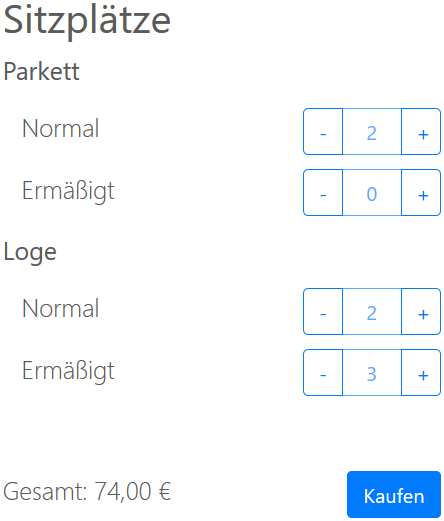
\includegraphics[width=0.4\textwidth]{img/screenshots/saalplan02}
	\captionsetup{format=hang}
	\caption{Preisstufen}
	\label{fig:saalplan02}
\end{figure}

Wählt man nun Sitzplätze aus, so muss man noch angeben, wie viele Tickets zum normalen Preis man kaufen möchte und wie viele zu einem ermäßigten Preis.
Daraus wird dann direkt der Preis berechnet und angezeigt (siehe Abbildung \ref{fig:saalplan02}).
Je nach Bildschirmgröße und -dimensionen werden diese Element neben dem Saalplan oder darunter angezeigt.
Mit dem \enquote{Kaufen}-Button gelangt man dann zur nächsten Seite, um weitere Daten anzugeben.

In der ersten Implementierung wurden der Saal und die Sitzplätze mit absoluten Größenangaben definiert.
So hatte das \textit{div}-Element, das einen Sitzplatz darstellt, als Höhe und Breite \textit{20px} gesetzt und eine Position relativ zur links oberen Ecke des Saals in Pixeln angegeben.
Die Koordinaten kommen dabei direkt aus dem Back-End bzw. der Datenbank.
Dies ermöglicht es, nicht nur einfach alle Plätze nebeneinander anzuzeigen, sondern auch Gänge einzufügen, Plätze versetzt anzuordnen, die Abstände zwischen den Sitzen individuell zu gestalten und somit den Saalplan an die Realität anzupassen.

Durch die Verwendung absoluter Größen in Pixeln, ist jedoch das Benutzererlebnis auf kleinen Bildschirmen schlechter.
Der Saal ist erst einmal breiter als der Bildschirm und der Benutzer muss herauszoomen und die Größe selbst anpassen.
Das Gleiche gilt für Benutzer eines Desktop-Computers, wenn sie die Fenstergröße anpassen.

Um dies zu verbessern, wird beim erstmaligen Laden sowie bei jeder Änderung der Fenstergröße, die Größe des Saals und der Sitzplätze neu berechnet.
Die Größenangaben aus der Datenbank werden dabei genutzt und entsprechend skaliert, sodass der Saalplan weder die volle Breite, noch die volle Höhe des Bildschirms überschreitet.
Um den Berechnungsaufwand zu reduzieren, sind die Koordinaten aller Sitzplätze prozentual angegeben.
Diese prozentualen Angaben beziehen sich dabei auf den \textit{div}-Container, der den Saal darstellt.
Dementsprechend muss lediglich die Größe des Saals und die Größe der Sitzplätze berechnet werden.

Ein Sitzplatz wird durch eine \acs{HTML}-Vorlage erstellt.
Die aus der Datenbank stammenden und in JavaScript verarbeiteten Werte werden zunächst in die Vorlage und im Anschluss ins \acs{DOM} eingefügt.

\begin{lstlisting}[style=lstHTML, caption={\acs{HTML}-Vorlage für die Darstellung eines Sitzplatzes}, label={lst:html_template_seat}]
<div id='`\textcolor{red}{\{seatID\}}`'
	class='seat `\textcolor{red}{\{classes\}}`'
	style='left: `\textcolor{red}{\{posx\}}`%; top: `\textcolor{red}{\{posy\}}`%;'
	title='`\textcolor{red}{\{tooltip\}}`'>
</div>
\end{lstlisting}

Die Gestaltung erfolgt dabei vollkommen über \acs{CSS}-Klassen, die in JavaScript hinzugefügt oder entfernt werden.

\begin{lstlisting}[style=lstCSS, caption={Optische Gestaltung der Sitzplätze}, label={lst:css_seat}]
.seat {
	border: 1px solid black;
}
.available {
	background-color: #0d0;
}
.occupied {
	background-color: #ccc;
}
.hovering {
	background-color: #0f0;
}
.selected {
	background-color: #55f;
}
\end{lstlisting}

\subsection{Reaktion auf Benutzerinteraktion}

Sobald der Benutzer einen Sitzplatz anklickt, wird diese Information an die zugehörige Funktion weitergereicht.

\begin{lstlisting}[language=JavaScript, caption={Erkennen des Anklickens eines Sitzplatzes}, label={lst:js_onclick}]
$(".seat").on("click", function () {
	var seatId = $(this).attr("id");
	if (seatId in selection) {
		removeSeatFromSelection(seatId, this);
	}
	else {
		addSeatToSelection(seatId, this);
	}
});
\end{lstlisting}

Wenn der Benutzer einen Sitzplatz auswählen möchte, muss noch einmal überprüft werden, ob dieser auch wirklich noch frei ist.
Zusätzlich soll der Sitzplatz für den Benutzer vorgemerkt werden, damit in der Zwischenzeit kein anderer den Sitzplatz reserviert.

Dafür wird eine \acs{AJAX}-Anfrage an das Back-End gesendet.
Dabei wird einerseits die Vorstellung und der ausgewählt Sitzplatz mitgegeben, andererseits aber auch eine Benutzeridentifizierung in Form einer zufälligen Zeichenkette, die im Browser des Benutzers als Cookie gespeichert wird.

\begin{lstlisting}[language=JavaScript, caption={Senden einer Anfrage, den Sitzplatz zu blocken}, label={lst:js_ajax_send_block}]
function addSeatToSelection (seatId, seatObj) {
	// prepare data for ajax
	var block = {show: {id: urlparameters.get("id")},
	             seat: {id: seatId},
	             sessiontoken: cookie};
	// send ajax
	var data = "block=" + JSON.stringify(block);
	$.ajax({
		type: "POST",
		url: "http://localhost:8080/cinema-system/reservation/block",
		data: data,
		contentType: "application/json; charset=utf-8",
		success: (data) => processBlockingResult(data, seatId, seatObj),
		error: function (xhr,status,error){
			console.log(xhr, status, error);
			processBlockingResult(null, seatId, seatObj);
		}
	});
}
\end{lstlisting}

Die Antwort des Servers wird an die entsprechende Funktion weitergegeben.
Dort wird nun überprüft, ob das Blocken des Sitzplatzes erfolgreich war oder nicht.

\begin{lstlisting}[language=JavaScript, caption={Verarbeiten der Server-Antwort beim Versuch, einen Platz zu blocken}, label={lst:js_ajax_process_block}]
function processBlockingResult (data, seatId, seatObj) {
	if(data != null) {
		var seatIdResponse = data.seat.id;
		seats[seatId].isBlocked = false;
		$(seatObj).addClass("selected available");
		$(seatObj).removeClass("occupied");
		selection[seatIdResponse] = true;
		numberOfTickets[getCategoryOfSeat(seatIdResponse)] += 1;
		updatePriceBox();
	} else {
		seats[seatId].isBlocked = true;
		$(seatObj).removeClass("available hovering");
		$(seatObj).addClass("occupied");
	}
}
\end{lstlisting}

Zum einen werden alle nötigen Variablen aktualisiert, zum anderen wird die Benutzeroberfläche entsprechend angepasst.
Dies umfasst den angeklickten Sitz selbst und auch die in Abbildung \vref{fig:saalplan02} gezeigten Auswahlmöglichkeiten für die Ermäßigung und Preisstufen der Sitzplätze. \\

Neben dem Auswählen der Sitzplätze, kann der Benutzer auch noch festlegen, wie viele Tickets zum normalen und wie viele zum ermäßigten Preis er kaufen möchte (siehe Abbildung \vref{fig:vorstellung02}).
Sobald der Benutzer einen solchen Knopf anklickt, wird die Verteilung von \textit{Normal} und \textit{Ermäßigt} in der einen Kategorie entsprechend angepasst.
Drückt man zum Beispiel bei \textit{Normal} auf \texttt{+}, so wird dort die Anzahl der Tickets um 1 erhöht und bei \textit{Ermäßigt} um 1 verringert.
Dies findet selbstverständlich nur statt, wenn dabei keine der Zahlen negativ wird bzw. die Anzahl der ausgewählten Sitze überschreitet.

Durch das Anpassen der Preisstufen ändert sich niemals die Anzahl der insgesamt ausgewählten Tickets.
Dies erfolgt lediglich durch das Selektieren bzw. Deselektieren im Saalplan.

\begin{figure}[ht]
	\centering
	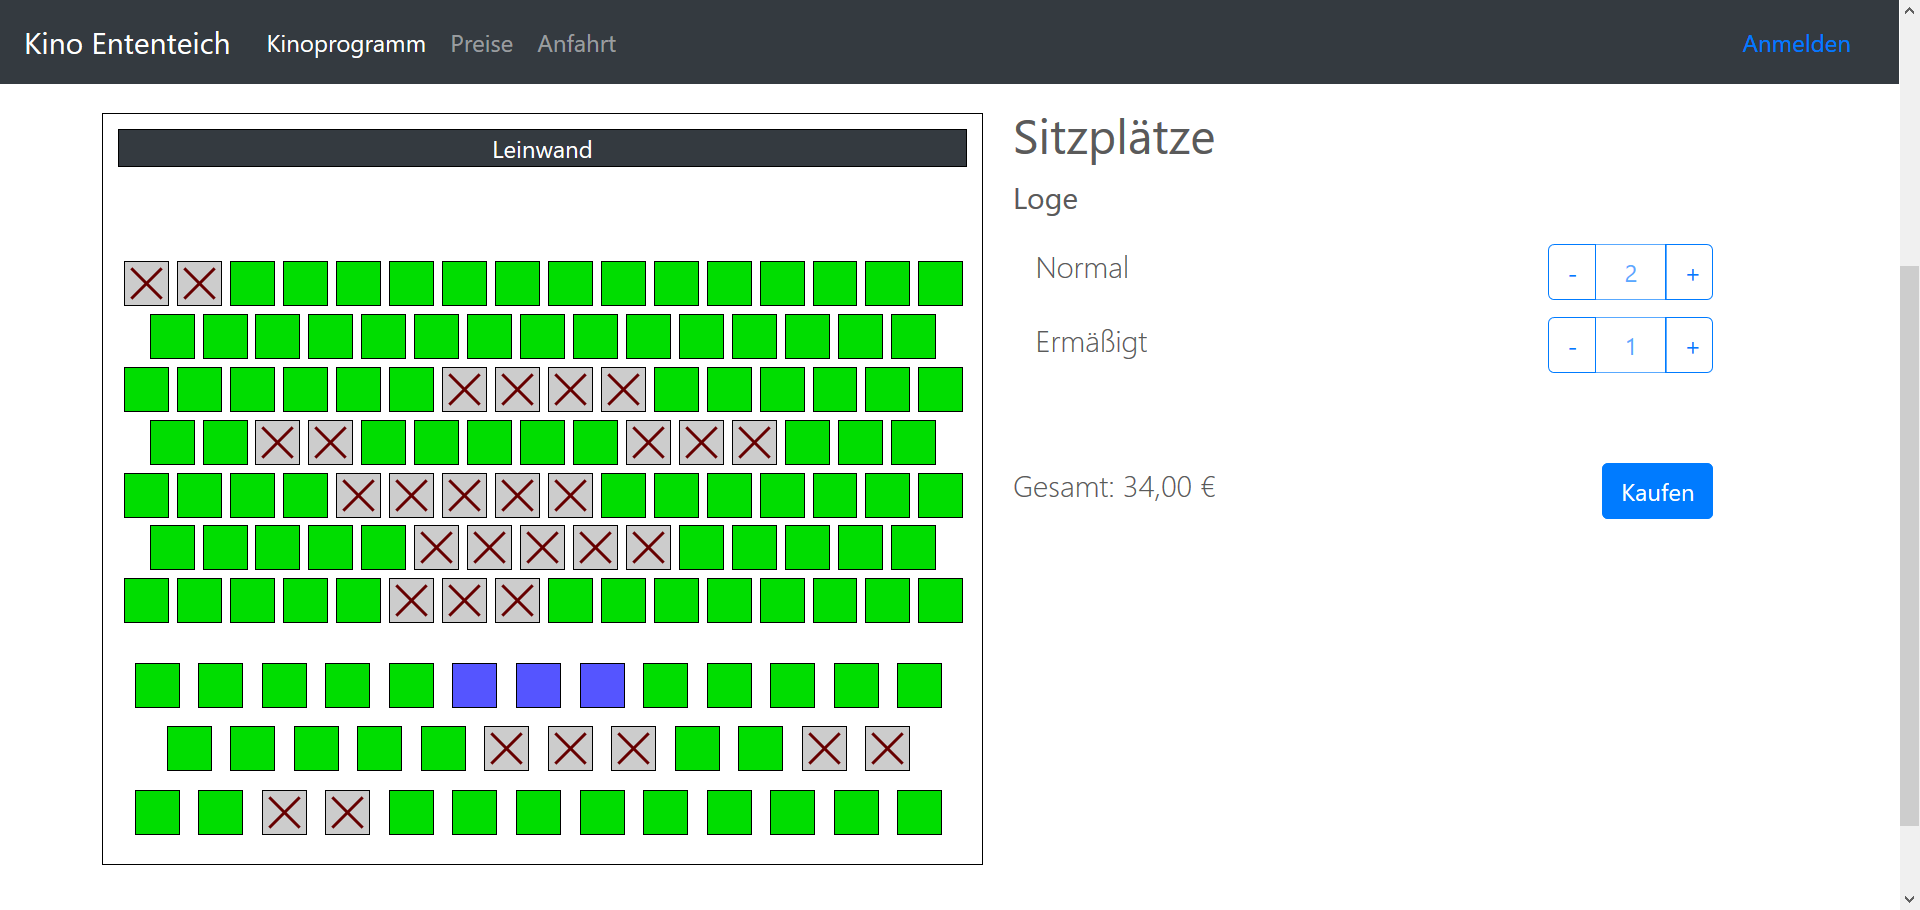
\includegraphics[width=0.95\textwidth]{img/screenshots/vorstellung02}
	\captionsetup{format=hang}
	\caption{Sitzplatzauswahl und Festlegung der Preisstufen}
	\label{fig:vorstellung02}
\end{figure}

% !TEX root =  master.tex
\section{Bezahlvorgang}

Wenn der Benutzer all seine Plätze ausgewählt hat und auch die Ermäßigungen angegeben hat, gelangt er zur nächsten Seite, auf der er weitere Daten eingeben muss.

\begin{figure}[ht]
	\centering
	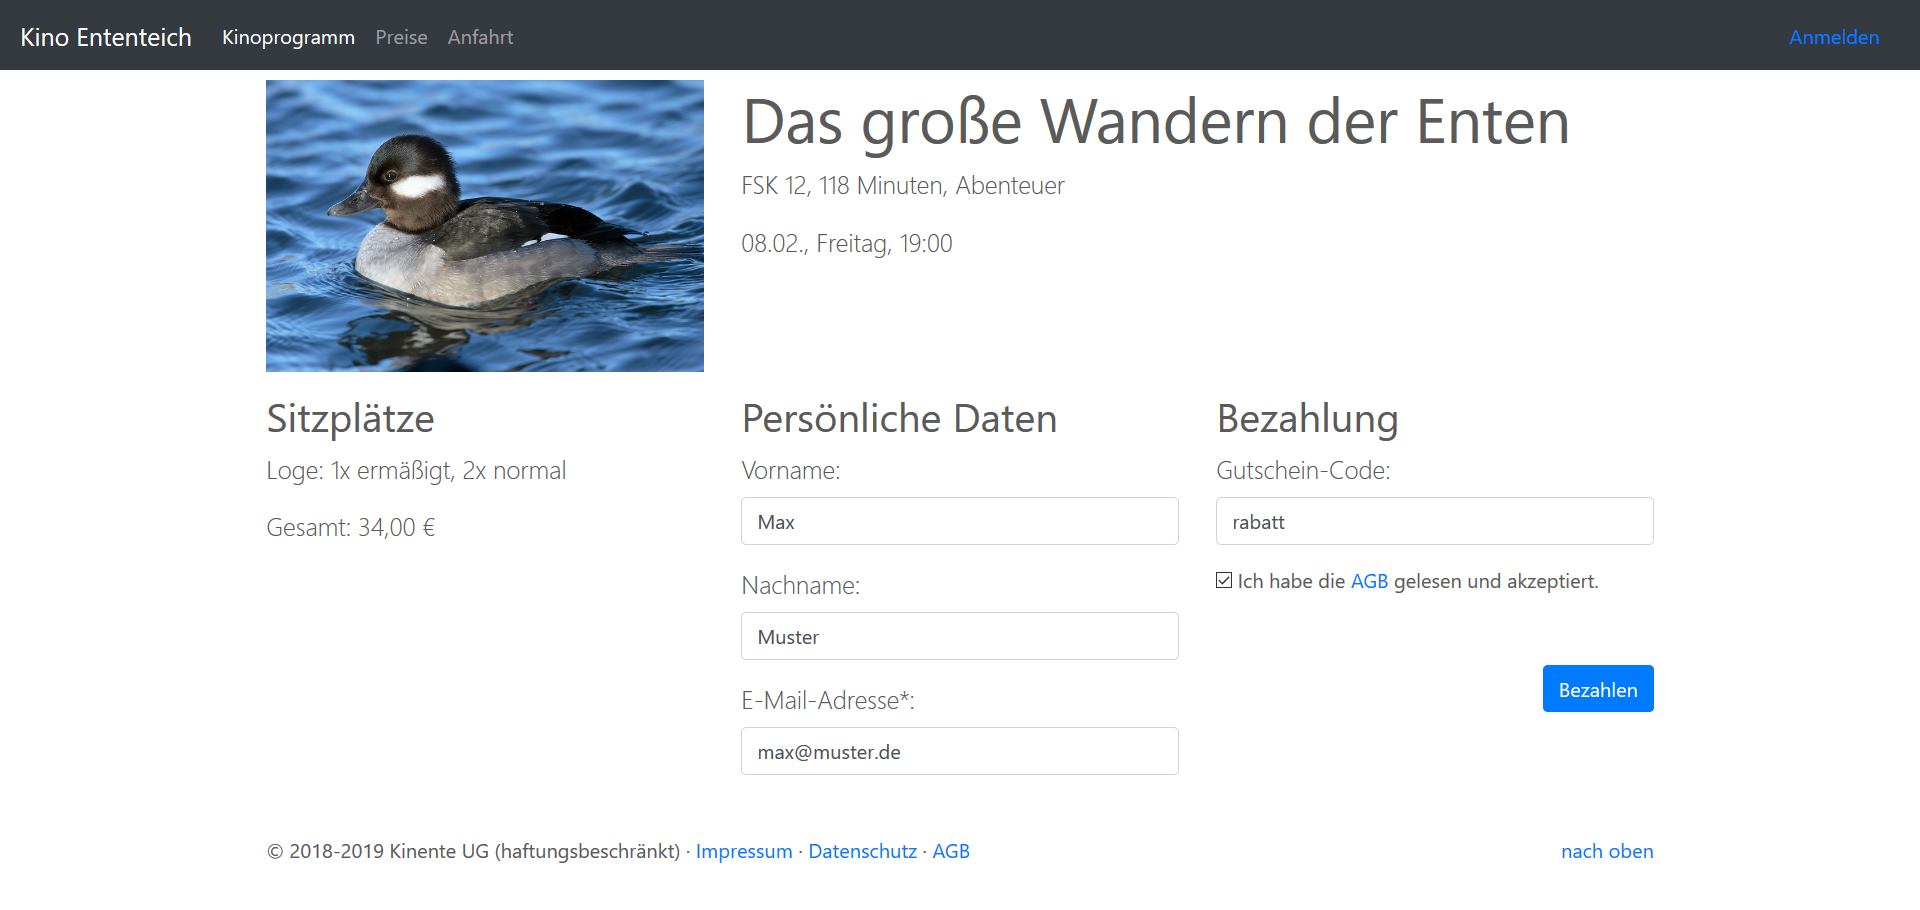
\includegraphics[width=0.95\textwidth]{img/screenshots/vorstellung03}
	\captionsetup{format=hang}
	\caption{Angabe weiterer Daten, die für den Buchungsvorgang relevant sind}
	\label{fig:vorstellung03}
\end{figure}

Die Daten zur Vorstellung, zu den ausgewählte Sitzplätzen, zu den Ermäßigungen und auch der Preis werden dabei über \acs{URL}-Parameter weitergegeben.
Auch wenn der Preis in diesem Fall redundant ist, so wird er trotzdem übergeben, um sich eine erneute Berechnung, die auch wieder eine weitere Kommunikation mit dem Back-End erfordern würde, zu ersparen.
Dies hat jedoch den Nachteil, dass der Benutzer Werte wie eben den Gesamtpreis theoretisch bei der Übergabe auf die nächste Seite ändern könnte und dann andere Werte angezeigt bekommt.
Dies betrifft jedoch nicht die Sicherheit des Systems, da alle Berechnungen und Überprüfungen zwangsläufig zumindest noch einmal im Back-End erfolgen müssen.
Am Beispiel des Preises würde dies bedeuten, dass der Benutzer zwar seine aktuelle Ansicht manipulieren kann, dennoch den korrekten Preis bezahlen muss.

Im oberen Bereich sieht der Benutzer nochmal allgemeine Informationen zur Vorstellung.
Des Weiteren erhält er eine Zusammenfassung zu seiner Sitzplatzauswahl mit dem Gesamtpreis.
Wenn sich der Benutzer entscheidet, die Sitzplätze verbindlich zu buchen, so wird im Hintergrund eine Nachricht an das Back-End gesendet.

Die Daten werden ähnlich wie beim Blocken eines Sitzplatzes in einem \acs{JSON}-Objekt gespeichert und mit einem \acs{AJAX}-Aufruf an das Back-End gesendet.

Im aktuellen Beispiel (siehe Abbildung \ref{fig:vorstellung02} und \ref{fig:vorstellung03}) würde sich dann folgendes \acs{JSON}-Objekt ergeben.

\begin{lstlisting}[language=JavaScript, caption={\acs{JSON}-Objekt für den Reservierungsvorgang}, label={lst:json_book}]
book = {paymentoption: "giftcard",
        verification: "rabatt",
        showId: 13,
        seats: [{id: 113, isReducedPrice: true},
                {id: 114, isReducedPrice: false},
                {id: 115, isReducedPrice: false}],
        customer: {firstname: "Max",
                   lastname: "Muster",
                   email: "max@muster.de"},
        sessiontoken: "TreevgQreNefpuUngHroreunhcgAvpugfTrznpug13"};
\end{lstlisting}

Neben den Informationen zur Vorstellung und den Sitzplätzen, wird auch noch die als Cookie gespeicherte Sitzungskennung mit angegeben.
Dies ist notwendig, damit eine Zuordnung zu den geblockten Sitzplätzen erfolgen kann.
Beim Auswählen des Sitzes wird der Sitzplatz für den Benutzer für eine gewisse Zeit geblockt.
Im Normalfall sind die Plätze beim Reservieren somit immer noch durch den Benutzer geblockt.
Durch die Angabe derselben Sitzungskennung, die auch beim Blocken verwendet wurde, ist es nun im möglich, dass im Back-End erkannt wird, dass der aktuelle Benutzer berechtigt ist, die geblockten Plätze zu reservieren.

Bei erfolgreicher Reservierung erhält man Informationen zur Reservierung, wie z.B. die Reservierungsnummer und die Tickets.
In diesem Fall kann auch die Bestätigung angezeigt werden, andernfalls erscheint eine Fehlermeldung.

Die Bestätigung enthält noch einmal alle Informationen zur Vorstellung, zur Anzahl der Sitzplätze und zum gezahlten Kaufpreis.
Unter einer kurzen Beschreibung zum weiteren Verlauf findet der Benutzer sein Ticket in Form eines \acs{QR-Code}s.
In diesem ist ein eindeutiger Verweis auf die Reservierung und somit auf alle Tickets gespeichert.
Der \acs{QR-Code} wird dabei unter Zuhilfenahme einer quelloffenen Bibliothek\footnote{\url{https://github.com/nayuki/QR-Code-generator}} erzeugt.

\begin{figure}[ht]
	\centering
	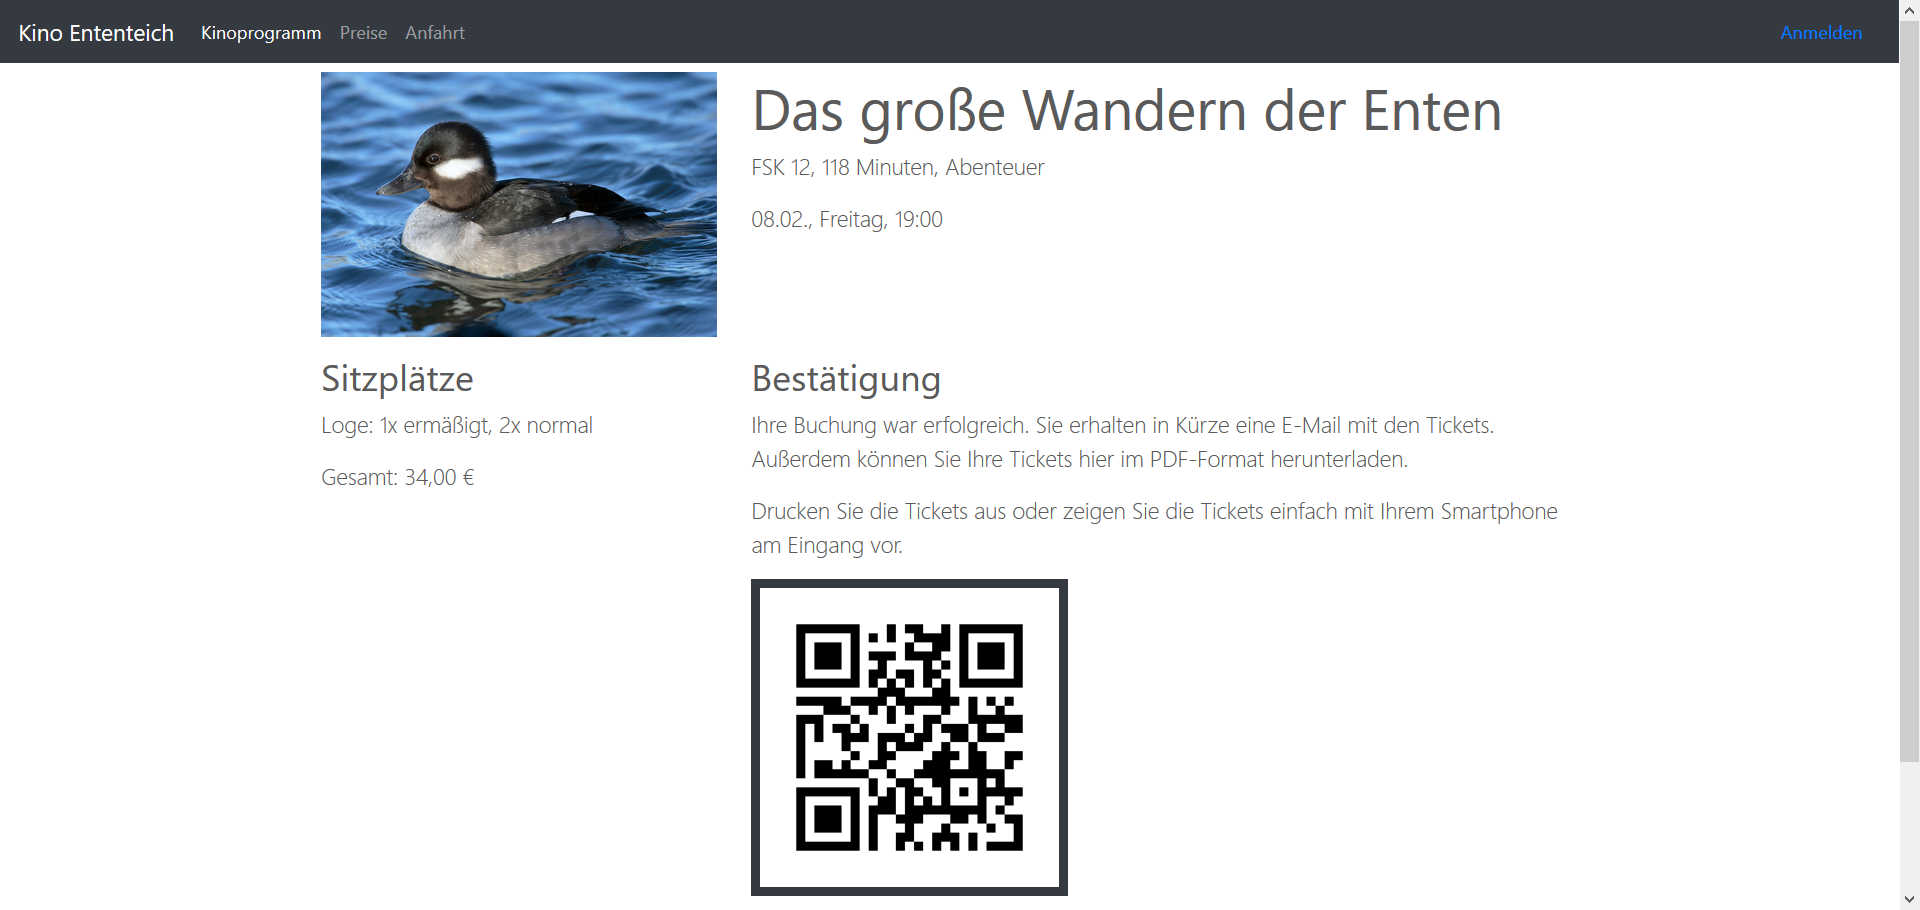
\includegraphics[width=0.98\textwidth]{img/screenshots/vorstellung04}
	\captionsetup{format=hang}
	\caption{Bestätigung einer Reservierung und Anzeige des \acs{QR-Code}s}
	\label{fig:vorstellung04}
\end{figure}

Im Kino kann an der Ticketkontrolle der \acs{QR-Code} gescannt und somit die Gültigkeit der Tickets überprüft werden.
Dadurch, dass ein \acs{QR-Code} für alle Tickets einer Reservierung steht, müssen sich die Benutzer, wenn sie mit mehreren Personen das Kino besuchen, keine Gedanken machen, wer welches Ticket erhält und die Tickets nicht untereinander verteilen. % TODO: move to design/planning?


% !TEX root =  master.tex
\chapter{Testen}
\label{sec:testen}
\chaptermulitpleauthor{\authorRF}{\authorEJ}
% !TEX root =  master.tex
\section{Softwarequalität}
\authorsection{\authorEJ}

Die Softwarequalität eines Programmes ist durch verschiedene Merkmale definiert.
Zu diesen gehören Funktionalität, Portabilität, Zuverlässigkeit, Benutzbarkeit, Effizienz und Wartbarkeit.\footnote{\url{https://entwickler.de/online/agile/softwarequalitaet-so-misst-und-verbessert-man-software-114867.html}}
Ebenfalls geht es dabei um die Erfüllung der Erwartungen eines Benutzers an das Programm.
In dem Fall, der für das Fach Fallstudie gestellten Anforderungen, handelt es sich um ein Kinoreservierungssystem, das über Front-End und Back-End steuerbar sein soll.
Diese Qualitätsmerkmale sind wichtig einzuhalten, da sie die Zufriedenheit bei Kunden sowie Programmierern erhöhen, die Zuverlässigkeit der Software steigern, einen reibungsloseren Betriebsablauf gewähren, Kundenwünsche zuverlässiger erfüllt werden können, die Anforderungen besser und angepasster nach den Wünschen des Kunden erfüllt werden können und die Arbeitsprozesse beim Programmieren der Software effektiver gestaltet werden können. % TODO: this sentence is hard to understand
Im Allgemeinen ist Testen also nicht nur für den Kunden der Software wichtig, sondern auch für die Programmierer.
Es bietet beiden Parteien Sicherheit, um mit der Software zu arbeiten und diese zu verwalten.
Dabei ist jedoch zu beachten, dass die Eliminierung von Fehlern mittels Testen immer aufwendiger wird.
Je mehr Code bereits durch Tests abgedeckt wurde, desto teurer wird die Erhöhung der Testabdeckung.
Der zu testende Code wird schwieriger zu testen und die Testerfolge sind nur noch kleinschrittig.
Am Ende übersteigen die Kosten für das Testen einer Codezeile deren Nutzen.
Um für dieses Problem eine Lösung zu finden gibt es das Qualitätsmanagement, es ist dafür da um ein Optimum aus Fehlerkosten und Fehlerverhütungskosten zu finden.
Diese lassen sich zwar nicht genau bestimmen, aber können trotzdem durch Erfahrungswerte, Vergleichswerte und abschätzende Planung mithilfe von Soll- und Istwerten etwas eingegrenzt werden.\footnote{\url{http://www.enzyklopaedie-der-wirtschaftsinformatik.de/lexikon/is-management/Systementwicklung/Management-der-Systementwicklung/Software-Qualitatsmanagement}}
Deshalb ist in den meisten Projekten keine Testabdeckung von 100\% gefordert, sondern es wird sich zwischen Kunde und Programmierer auf einen niedrigeren Prozentsatz geeinigt.
Für das Kinoreservierungsprogramm wird eine Codeabdeckung von $\sim$60\% gefordert und in Kapitel \vref{sec:codeabdeckung} nochmal näher beschrieben.

% !TEX root =  master.tex
\section{Testverfahren}
\authorsection{\authorEJ}

Testen wird oftmals als Prozess, der aufzeigen soll, dass keine Fehler in dem Programmcode vorhanden sind, fehl verstanden.
Im eigentlichen Sinne geht es dabei nicht darum zu zeigen, dass der Quellcode fehlerfrei ist, sondern das er Fehler enthält und nach diesen gesucht werden muss.\footnote{\url{http://www.knaupes.net/theorie-der-softwaretests/}}

\subsection{Testprinzipien}
Aufgrund dieser Definition für Testen müssen Ausgangsvoraussetzungen gegeben sein, um eine möglichst umfangreiche Testabdeckung gewährleisten zu können.
Zu diesen zählen das Feststellen, ob der Quellcode genau die Anforderungen erfüllt und sonst auch keine weiteren Eventualitäten abdeckt.
Ebenfalls sollte dabei genau dokumentiert werden, welcher Testfall bereits abgedeckt wurde, da bei vielen unterschiedlichen Testfällen und einem größeren Testpensum der Überblick schnell verloren werden kann.
Des Weiteren müssen Testfälle reproduzierbar sein und es darf sich nicht um ein einzelnes Phänomen handeln.
Einen Testfall zu generieren, der aber eigentlich gar nichts mit dem zu testenden Quellcode zu tun hat, ist einerseits nicht möglich und andererseits nicht sinnvoll.
Der aber wohl wichtigste Punkt, ob fachlich oder menschlich gesehen, ist jedoch, dass der Tester nicht der Programmierer selbst sein darf.
% TODO: streitbare Aussage (normalerweise wird der Test geschrieben, bevor der entsprechende Code vorhanden ist; dadurch ist die folgende Argumentation teilweise hinfällig)
Als Programmierer des Quellcodes besitzt man eine voreingenommene Meinung, der Quellcode hat genau einen Zweck und diesen erfüllt er für den Programmierer auch.
Daher kann ein größerer Blickwinkel auf den Quellcode leider nicht gewährleistet werden und die Testfälle können nicht in hinreichender Genauigkeit generiert werden.
Ebenfalls hat ein Tester auch keine leichte Aufgabe, da er sich in den Quellcode des Programmierers einarbeiten und diesen testen muss.
Damit ist es aber noch nicht getan, da der Tester nun den Fehler weitergeben muss.
Das absichtliche Suchen nach Fehlern und der Drang nach Perfektionismus ist zwar notwendig, kann aber schnell zu zwischenmenschlichen Konflikten führen.
Deshalb ist sowohl auf Tester- und Programmierseite Vorsicht und auch Verständnis für die Aufgabe des Gegenparts geboten.

\subsection{Äquivalenzklassen}
Da selbst bei einem einfachen Test die möglichen Testfälle unmöglich viele werden können, kann durch die Äquivalenzklassen Abhilfe geschaffen werden.
Diese Äquivalenzklassen verhalten sich gleich wie die getesteten Eingabedaten, daher kann man davon ausgehen, dass diese Testfälle ebenfalls abgedeckt wurden.
In diesem Sinne reicht es die Grenzfälle zu testen und bei allen anderen Möglichkeiten von einer äquivalenten Verhaltensweise auszugehen.\footnote{\url{https://wr.informatik.uni-hamburg.de/_media/teaching/wintersemester_2010_2011/siw-1011-ehmke-tests-ausarbeitung.pdf}}
Um dies mit einem Beispiel zu erläutern, könnte man die Subtraktion von zwei Zahlen heranziehen.
Wenn also die Subtraktion von Zahlen in einem Testfall funktioniert hat, dann kann man davon ausgehen, dass die anderen möglichen Testfälle mit Eingabedaten des gleichen Datenformates und Datentyps auch ein positives Ergebnis zurückgeben werden.

\subsection{Testebenen}
Das Testen von Quellcode kann in vielen Weisen passieren.
Einerseits kann der Quellcode an sich getestet und damit jede einzelne Komponente einer Anwendung überprüft werden, auch Komponententests bezeichnet.
Diese Ebene kann durch ein besonderes Designparadigma auch zur leitenden Kraft der Softwareentwicklung werden, dies ist die testgetriebene Softwareentwicklung.
Dabei wird meistens Nutzen aus den Vorteilen einer agilen Softwareentwicklung gezogen, um am Ende ein Konglomerat von positiven Effekten zu erhalten.
Diese stellen sich durch höhere Qualität, niedrigere Wartungsarbeiten, saubere Struktur und effektive Vermeidung von Redundanzen ein.\footnote{\url{https://de.ryte.com/wiki/Test_Driven_Development}}

Auf der nächsten Stufe folgen dann die Integrationstests. Diese sind dazu da, um Redundanzen innerhalb des Projektes aufzudecken.
Ebenfalls können nicht eindeutige Spezifikationen der Klassen bemerkt und ausgemerzt werden.

Danach kommen noch die System- und Abnahmetests, diese sind beide durch einen gemeinsamen Nenner definiert.
Beiderseits wird die Prüfung nach der Zufriedenstellung der Systemanforderungen realisiert.
In Detail handelt es sich bei den Systemtests um diverse Performance-, Installations-, Wiederinbetriebnahme-, Stress- und Usability-Tests.
Auf der anderen Seite wird bei einem Abnahmetest geprüft, ob die Anforderungen eines Benutzers erfüllt werden und die Funktionalität, User Experience und Dokumentation in einer angemessenen Art und Weise erfüllt wurden.\footnote{\url{https://wr.informatik.uni-hamburg.de/_media/teaching/wintersemester_2010_2011/siw-1011-ehmke-tests-ausarbeitung.pdf}}

\subsection{White-Box-Test und Black-Box-Test}
Bei beiden Testformen handelt es sich um eine Art den Quellcode auf seine Struktur, Design und Implementation zu testen.
In einem Black-Box-Test hingegen ist der zu testende Code nicht bekannt und dies ist auch nicht erwünscht.
Es handelt sich um eine einfache und billige Art und Weise das System zu testen.
Der Programmierer muss dabei keinerlei Kenntnisse von der Implementierung haben, sondern lediglich die Anforderungen an das System kennen.
Die möglichen Testmethoden sind Akzeptanz- und System-Tests, also Tests, ob die Anforderungen des Benutzers und die Anforderungen an das System erfüllt wurden.
Als Beispiel kann man sich einen Tester für ein Kinobuchungssystem vorstellen, der als Testfall das Buchen von Eintrittskarten heranzieht.
Er besitzt weder Kenntnisse über das System, noch hat er eine konkrete Ahnung, welche Brennpunkte in dem System existieren und wird diese auch nicht explizit testen.

Im Gegensatz dazu gibt es noch die White-Box-Test.
Dabei handelt es sich um das Gegenteil eines Black-Box-Tests.
Diese Methode ist im Gegensatz zu einem Black-Box-Test teurer und aufwendiger, aber führt zu einer genaueren Testabdeckung.
Der Tester hat detaillierte Kenntnisse über das System und hat Einblick in alle Ressourcen, die den Quellcode betreffen.
Die Testmethoden eines White-Box-Testers sind Unit-Tests und Integrationstests, also Test auf die Verwendung von Codeabschnitten und einzelnen Codezeilen.
Das Beispiel für einen solchen Test wäre ein Tester, der jede Zeile eines Kinobuchungssystems auf Herz und Nieren testet.

% !TEX root =  master.tex
\section{Technische Grundlagen der Tests}
\authorsection{\authorRF}

\subsection{JUnit}

\subsubsection{Allgemeines}

JUnit ist ein Java-Framework, welches vorwiegend zum Automatisieren von Tests verschiedener Klassen und Methoden verwendet wird.\footnote{\url{https://junit.org/junit5/docs/current/user-guide/}}

Ein Test kann bei JUnit zwei Ergebnisse erzielen, entweder er schlägt fehl und wird mit rot markiert oder er läuft erfolgreich ab und wird grün markiert.
Bei den fehlgeschlagenen Tests wird jedoch noch weiter unterschieden.
Es gibt sogenannte \enquote{Failures}, welche dadurch charakterisiert sind, dass nicht das erwartete Ergebnis beim Test aufgetreten ist.
Des Weiteren gibt es sogenannte \enquote{Errors}, welche unerwartete Fehler sind, die während eines Tests auftreten können und somit den Test möglicherweise nicht vollenden lassen oder ein falsches Ergebnis hervorrufen.

Tests werden zudem als eigene Klassen realisiert, um sie vom Programmcode abzugrenzen und nicht vor dem Kompilieren des Projektes entfernen zu müssen.

\subsubsection{Funktionsweise}

JUnit-Tests werden in Java mit Annotationen angekündigt und können mit diesen spezialisiert werden.
Standardmäßig wird ein Test mit \enquote{@Test} eingeleitet, danach folgt die eigentliche Test-Methode.
In der Test-Methode werden die zu testenden Klassen bzw. Methoden aufgerufen und mit Hilfe der \textit{assertEquals}-Methode getestet.
Hierbei wird ein erwarteter Wert bzw. ein erwartetes Objekt angegeben und diese mit den Ergebnissen der zu testenden Methoden auf Gleichheit geprüft.

Falls mehrere Tests die selben Ausgangsdaten benötigen, kann mit Hilfe der \enquote{@BeforeAll}-Annotation einmalig zu Beginn bzw. mit \enquote{@BeforeEach} vor jeder Test-Methode eine Initialisierungsmethode eingeleitet werden, um die Ausgangsdaten zu erzeugen.
Gleichzeitig gibt es diese Annotationen auch nach den Tests, um bspw. Datenbankverbindungen zu schließen.
Diese Methoden werden mit \enquote{@AfterAll} und \enquote{@AfterEach} eingeleitet.

Außerdem können Tests übersprungen werden, sofern sie mit \enquote{@Disabled} eingeleitet werden.
Dies hat einerseits Vorteile bei der Entwicklung, da so Tests schneller geprüft werden können, andererseits können so Tests auskommentiert werden, sofern Bugs in den zu testenden Methoden vorhanden sind.


\subsection{Hamcrest}

Hamcrest ist wie JUnit ein Java-Framework, welches es leichter macht, richtige Matcher-Objekte zu deklarieren.
Jedoch ist Hamcrest als Zusatz zu JUnit zu betrachten und nicht als eigenständiges Test-Framework.
Dies ist ein großer Vorteil gegenüber dem Standard-Matcher von JUnit, da dieser allein mit der Gleichheit der Objekte arbeitet.
Somit ist es einfacher, komplette Kollektionen von Objekten auf Gleichheit zu testen oder komplexere Tests aufzustellen.

Hamcrest erlaubt es dem Nutzer zusätzlich auch eigene Matcher zu erstellen, welche das Testen erheblich erleichtern können.


% !TEX root =  master.tex
\section{Umsetzungen der Tests}
\authorsection{\authorRF}

\subsection{Vorwort}

Das Kinoreservierungsprogramm befindet sich noch in der Entwicklung, weshalb sich bei den Tests dafür entschieden wurde, keine Testdatenbank zu erstellen.
Durch diese Maßnahme wurde Zeit eingespart, welche in die weitere Entwicklung einfließen konnte.
Jedoch sind die Autoren der Arbeit sich bewusst, dass sobald das Programm veröffentlicht werden sollte, die Testdaten simuliert werden und somit keine Tests mit echten Daten in Bezug kommen sollten.

\subsection{Rollenverteilung}

Sofern Code und dazugehörige Tests von derselben Person bzw. Personengruppe entwickelt werden, entstehen oft im späteren Verlauf der Entwicklungsphase unerwartete Probleme.
Diese Probleme entstehen dadurch, dass Entwickler oft ähnliche Werte zum Testen verwenden, wie sie bei der Entwicklung bedacht haben.
Eigenständige Tester jedoch betrachten Tests unvoreingenommenen und verwenden andere Werte, welche vom Entwickler möglicherweise nicht bedacht wurden.
Zudem zwingt es die Entwickler des Back-Ends dazu, verständlichen Code bzw. dazugehörige Kommentare zu schreiben, da sonst die Entwicklung der Tests negativ beeinflusst werden kann.\footnote{\url{https://wr.informatik.uni-hamburg.de/_media/teaching/wintersemester_2010_2011/siw-1011-ehmke-tests-ausarbeitung.pdf}}

Dadurch, dass die Entwickler der Tests des Kinoreservierungsprogramms nur in moderatem Maß mit der Entwicklung des Back-Ends zu tun hatten, sind die Tests mit größtenteils unvoreingenommenen Ein-/Ausgabedaten entstanden.
Dies hat den Vorteil, dass diverse Szenarien betrachtet wurden, die bei der Entwicklung nicht bedacht worden sind.
Somit konnten Fehler des Back-Ends frühzeitig erkannt und behoben werden.


\subsection{Eigene Tests}

\subsubsection{Entitäten und Datentransferobjekte}

Da in dem Projekt \acsp{DTO} (siehe Kapitel \vref{sec:dto}) verwendet werden, um die Daten aus der Datenhaltungsschicht der Drei-Schichten-Architektur in die Logikschicht zu transferieren, müssen diese an geeigneten Stellen von \acsp{DTO} zu Entitäten bzw. von Entitäten zu \acsp{DTO} umgewandelt werden.
Dies geschieht mittels der \jinline |EntityToToHelper|- bzw. der \jinline |ToToEntityHelper|-Klasse.
Diese Umwandlung wird für beide Klassen in eigenen Testklassen getestet.
Beide Testklassen sind grundlegend gleich aufgebaut, da beide erst Test-Entitäten bzw. Test-\acsp{DTO} mit den exakt gleichen Attributen erstellen.
Danach wird verglichen, ob das durch die Umwandlung entstandene Objekt die exakt gleichen Attribute besitzt.
Zu sehen ist dies im Anhang \vref{src:entitytotohelpertest} anhand des Employee-\acsp{DTO}.
Im Code-Beispiel wird gezeigt, wie je ein \acs{DTO}-Objekt und ein Entitäts-Objekt erstellt wird und über \jinline |Set|-Methoden die exakt gleichen Werte übergeben werden.
In der nachfolgenden Test-Methode wird dann geprüft, ob bei der Eingabe von \texttt{NULL} kein Error entsteht, sondern \texttt{NULL} zurückgegeben wird.
Anschließend wird die Employee-Entität mit Hilfe der \jinline |EntityToToHelper|-Klasse umgewandelt und die jeweiligen Attribute werden überprüft, ob sie mit den Attributen des vorher erstellten Vergleichsobjekts übereinstimmen.
Dadurch werden alle \jinline |Getter|-Methoden getestet.
Zudem werden durch das Erstellen der Objekte zu Beginn der Testklassen alle \jinline |Setter|-Methoden der Entitäts- und \acs{DTO}-Klassen mit genutzt und überprüft.

\subsubsection{JSON-Konvertierung}

Das Überführen der Daten in das \acs{JSON}-Format ist ein wichtiger und entscheidender Schritt für die nahtlose Zusammenarbeit zwischen Front- und Back-End.
Deshalb wurde beim Testen der Konvertierungs-Klasse besonderen Wert auf Vollständigkeit gelegt.
In der Testklasse wurde daher die Konvertierung für jeden einzelnen \acs{DTO}-Typen vorgenommen und überprüft.
Dies ist zwar nicht direkt notwendig, da die Klasse sich für jeden \acs{DTO}-Typen gleich verhält, aber erhöht jedoch die Sicherheit, dass keine unbemerkten Fehler bei diesem Schritt entstehen, ungemein.


\subsubsection{Eigene Werkzeuge}

Neben der \acs{JSON}-Konvertierung wurden weitere Werkzeuge entworfen, um diverse Konvertierungen zu übernehmen.
Diese Werkzeuge befinden sich in der \jinline |Utils|-Klasse und erstrecken sich über Zeitkonvertierungen von Date-Objekten zu Strings, das Herauslesen von Informationen zum Datum oder Tag aus Strings oder verschiedene Überprüfungen, ob die Buchung eines Sitzplatzes erfolgreich ist.
Zum Testen dieser Methoden reicht es aus, vorher eigene Kalender-Objekte zu erstellen, diese umzuwandeln und mit vorher festgelegten Strings zu vergleichen.
Methoden zur Überprüfung, ob ein Sitz buchbar ist, wurden mit Hilfe von Sitz-Objekten und verschiedenen Zeitstempeln gebucht.
So ist ein Sitz für eine aktuelle Vorstellung nicht, aber für zukünftige Vorstellungen buchbar.

\subsubsection{Ressourcen}
Die Ressourcen des Fachkonzepts, namentlich \jinline|ReservationResource|, \jinline|ShowResource| und \jinline|MovieResource|, wurden auch komplett auf ihre Funktionalität getestet.
Hierbei wurde darauf geachtet, dass jede Anfrage überprüft wird.
Anhand der \texttt{Reservation\-Resource} wird nachfolgend das Testen erklärt.

Zu Beginn des Tests werden alle zur Reservierung benötigten \acs{DTO}-Objekte angelegt, also ein Kunde, ein Buchungsobjekt sowie eine zu buchende Show.
Nachdem das Buchungsobjekt mit Hilfe der \acs{JSON}-Konvertierung umgewandelt wurde, wird die \jinline |postTickets|-Methode der Ressource aufgerufen und der entstandene String übergeben.
Als Bestätigung, sofern das Buchen erfolgreich ist, wird ein Reservations-Objekt in Form eines \acs{JSON}-Strings übergeben.
Dieser String wird mit Hilfe der Konvertierungsklasse wieder zurück in ein Reservations-Objekt umgewandelt.
Danach wird aus dem entstanden Reservations-Objekt die ID entnommen und mit dieser geprüft, ob die Reservierung im System vorhanden ist.
Dies geschieht mittels der \jinline |getReservationById|-Methode und hat ein Reservations-Objekt als \acs{JSON}-String als Rückgabewert.
Dieser \acs{JSON}-String wird erneut zu einem Reservierungs-Objekt umgewandelt, um das Objekt mit dem vorher aus der Buchung erhaltenen Objekt zu vergleichen.
Damit wird sichergestellt, dass das Buchungs-Objekt auch alle Informationen enthält, die vorher abgegeben wurden.

Danach wird über die vorher ausgelesene ID die Reservierung gelöscht.
Dies geschieht über die \jinline |deleteReservationById|-Methode und gibt wie die anderen beiden Methoden das gelöschte Reservations-Objekt als \acs{JSON} zurück.
Diese \acs{JSON} wird wie zuvor auch in ein Objekt umgewandelt und danach überprüft, sodass alle Informationen korrekt sind.
Zu Überprüfung, ob die Reservierung auch erfolgreich gelöscht wurde, wird am Ende des Tests überprüft, ob eine Reservierung unter der vorher erhaltenen ID vorhanden ist.

Zusätzlich wird in der \jinline |ReservationResource| das Blockieren und Deblockieren einzelner Sitze ausgeführt.
Um dies zu testen werden zwei Blockierungs-Objekte zu Beginn des Tests angelegt.
Diese bestehen aus einer eigenen ID, einem Sitz, der blockiert werden soll, einem Sessiontoken und einer dazugehörigen Show, in der der Sitz blockiert werden soll.
Im Test wird so ein Sitz blockiert und wieder freigegeben, bei beiden Operationen wird ein Block-Objekt im \acs{JSON}-Format übergeben.
Diese Objekte werden anschließend auf ihre Gleichheit überprüft, um sicherzustellen, dass der blockierte Sitz mit dem freigegebenen Sitz übereinstimmt.

Die Tests der \jinline |ShowResource| und der \jinline |MovieResource| sind analog zum beschriebenen Test zu erklären.
Jedoch sind die beiden anderen Ressourcen auf das Auslesen von Daten spezialisiert und konnten somit leichter getestet werden.
Lediglich in der \jinline |MovieResource| befindet sich ein weiterer \jinline |Post| von Daten.
Dieser wurde ähnlich des \jinline |Posts| der Reservierung umgesetzt, mit dem Nachteil, dass ein Löschen eines Filmes im aktuellen Entwicklungsstand nicht möglich ist.
Dies muss per Hand nach dem Test gelöscht werden, da sonst ein Test-Film in der Datenbank steht.

\subsection{Codeabdeckung} 
\label{sec:codeabdeckung}
Für das Kinoreservierungsprogramm wurde bezüglich des Testens vorgeben, dass eine Codeabdeckung von 60\% erreicht werden soll.
Jedoch beziehen sich diese 60\% nur auf den eigenen logischen Code.

Durch die erstellten Tests werden $\sim$70,7\% des gesamten Codes der Datenhaltung und $\sim$65,9\% des gesamten Codes des Fachkonzepts abgedeckt.
Somit wurden die Vorgaben nicht nur erreicht, sondern übertroffen.

Durch die Tests der verschiedenen Ressourcen des Fachkonzepts werden die dazugehörigen Services mit getestet.
Ein Testen der einzelnen Services im Back-End wurde durch die Komplexität des Projektes als nicht ökonomisch sinnvoll erachtet und aus zeitlichen Gründen nicht durchgeführt.
In Kapitel \vref{sec:konzept} wird der Zusammenhang der Fachkonzeptschicht mit der Datenhaltungsschicht erläutert.
Dieser Zusammenhang trägt auch zur Testabdeckung bei, wird jedoch durch die verwendete \acs{IDE} nicht dargestellt.
Somit kann jedoch nicht genau gesagt werden, um welchen Betrag sich die Testabdeckung des Datenhaltungs-Codes steigern würde.


% !TEX root =  master.tex
\chapter{Ausblick}
\label{c:ausblick}
\chaptermulitpleauthor{\authorRF}{\authorEJ, \authorSG, \authorNL}
% !TEX root =  master.tex
\section{Zukünftige Sprints und Backlog}

\subsection{Theoretischer Sprint 3}
\label{ssec:theoretischer_sprint}
\multipleauthorsection{\authorRF}{\authorEJ, \authorNL}

% !TEX root =  master.tex
\section{Abgeschlossene und offene Ziele der Software}
\multipleauthorsection{\authorRF}{\authorEJ}
\label{sec:ziele}
\subsection{Zieldefinition}
\subsubsection*{Ziel}
Das Ziel der Arbeit war es, ein Kinobuchungssystem zu entwickeln, welches dem Benutzer ermöglicht eine Buchung durchzuführen.
Dieses Kinobuchungssystem sollte mit Hilfe der iterativen Vorgehensweise entwickelt werden.
\subsubsection*{Vorgaben}
Eine Einschränkung des Entwurfs- und Entwicklungsprozesses war die Vorgabe, die Programmiersprache Java im Back-End (vgl. Kapitel \vref{sec:backend}) zu verwenden sowie den Entwicklungsprozess innerhalb von zwei Sprints und einem Bearbeitungszeitraum von zwölf Wochen abzuschließen.
Zudem sollten ca. 60\% des eigenen logischen Codes durch Tests abgedeckt werden. Dies bezieht sich lediglich auf das Back-End und den Businesscode des Projektes.

\subsubsection*{Eigene Ziele}
Unsere eigenen Ziele waren die Verwendung einer Datenbank, um die Voraussetzungen einer Drei-Schichten-Logik zu erfüllen.
Dies sollte den Austausch von Daten im System erleichtern.

Weiterhin sollte es möglich sein einen kompletten Buchungsvorgang durchzuführen, d.h. von der Filmauswahl über die Vorstellungsauswahl sowie die Sitzplatzauswahl bis hin zur Buchung und deren Bestätigung zu gelangen.
Während des Buchungsvorganges soll dem Benutzer eine unverkennbare User Experience geboten werden, welche eine erneute Verwendung des Kinobuchungssystems begünstigt.

\subsection{Abgeschlossene Ziele}
\label{ssec:abgeschlossene_ziele}
Das vorliegende Kinoreservierungssystem erfüllt alle an das Projekt gestellten Zielvorgaben und überschreitet diese an diversen Stellen. 

\subsubsection*{Back-End}
Das komplette Back-End wurde innerhalb der zwei Iterationen mit eine Datenbank sowie der geforderten Businesslogik implementiert. Ferner wurden neue Architekturmuster sowie die Implementierung von Webservices inklusiver deren \acs{REST}-Schnittstellen implementiert. Da diese Themen noch nie in einer Vorlesung thematisiert wurden, übertrifft dies die an das Projekt gestellten Anforderungen. Darin beinhaltet ist eine Restriktion der mehrmaligen Buchung eines Sitzplatzes sowie das temporäre Blockieren eines online ausgewählten Sitzplatzes.

\subsubsection*{Front-End}
Im Front-End wurden alle geplanten Schritte der Buchung implementiert. 
Somit kann der Nutzer von der Filmauswahl bis zur Buchung ohne Unterbrechung die Funktionsweise eines Kinoreservierungssystems in Anspruch nehmen. Dies wird jedoch aktuell durch eine vorgegebene Zahlungsmethode, welche nur vorher festgelegte Werte erlaubt, limitiert.

\subsubsection*{JUnit}
Das Testen wurde, wie in Kapitel \vref{sec:testen} beschrieben, auch im Rahmen der Vorgaben erfüllt. Hierbei wurde das Ziel überschritten, da die zu testenden Klassen eine höhere Codeabdeckung als gefordert aufweisen.

\subsubsection*{Datenbank und \acf{REST}}
%Die eigenen Ziele wurden ebenfalls zum großen Teil erreicht. 
Das Verwenden einer Datenbank wurde mit Hilfe einer Postgres-Datenbank umgesetzt.
Hierzu wurden sämtliche von den Autoren festgelegten Attributen im Backend implementiert und für die weitere Verwendung bereitgestellt.\\
Durch die Implementierung von einem breiten Schnittstellen-Portfolio, die sowohl Speichern, Abrufen und Löschen mit Hilfe von \acs{REST}-Services ermöglichen, wird eine umfangreiche Kommunikation zwischen Front- und Back-End gewährleistet. \\
Somit wurde das Ziel, einer klaren Trennung in Form der Drei-Schichten-Logik, erreicht.

\subsubsection*{Buchungsvorgang und Sitzplatzauswahl}
Ein weiteres, selbst gestecktes Ziel war es einen erfolgreichen Buchungsvorgang, wie in der User-Journey (siehe Kapitel \vref{sec:user_journey}) beschrieben, zu durchlaufen.
Hierbei wurde im Front-End zusätzlich zur geplanten Filmauswahl ein Karussell mit aktuellen Blockbustern als Eye-Catcher implementiert. \\
Darüber hinaus wurde die Sitzplatzauswahl im Front- und Back-End gegenüber einer konventionellen Anordnung in Tabellenform durch ein Koordinatensystem ersetzt.
Folglich ergeben sich diverse Möglichkeiten, die sich zu einer realitätsgetreuen Darstellung aller denkbaren zweidimensionalen Sitzplatzanordnungen abbilden lassen. 
Ferner wird die Skalierbarkeit im Hinblick auf der Größe der Säle bzw. Anzahl der Plätze gewahrt. 

\subsubsection*{Hauptziel}
Der Hauptziel dieses Projekts war es, einen Sitzplatz einer Vorstellung nicht mehrmals zu verkaufen.
Dies wurde mit Hilfe des temporären Blockierens eines Sitzes gelöst.  
Eine genauer Beschreibung des genannten Ansatzes befindet sich in Kapitel \vref{ssssec:geblockt_durch_benutzer}. \\

Schlussendlich wurde auch bereits der Grundstein des theoretischen dritten Sprints gelegt, indem ein Mitarbeiter im Back-End bereits implementiert wurde.

\subsection{Offene Ziele}
\label{ssec:offene_ziele}
\subsubsection*{Sitzplatzdarstellung}
Zu den offenen Zielen, welche nicht in voller Gänze erreicht wurden, zählt die Sitzplatzdarstellung.
Diese sollte nach Plan auch eine Breite und Höhe in der Datenhaltung aufweisen, um jegliche Sitzarten (Sofas etc.) darstellen zu können.
Des Weiteren fehlt die Spezifikation für Rollstuhlplätze, diese werden in der aktuellen Version nicht dargestellt.
Jedoch ist das Potential für diese Änderungen im aktuellen System vorhanden, weshalb sie bei einem größeren Bearbeitungszeitraum auch erreicht worden wären.

\subsubsection*{Single-Page-Application}
Ein weiteres offenes Ziel ist die Umsetzung des Front-Ends als Single-Page-Application, hierbei wäre redundanter Datenaustausch verhindert worden.
Es wurde sich jedoch aufgrund Zeitmangels gegen eine frühzeitige Konvertierung des Front-Ends entschieden, um Ressourcen für Anpassungen im Back-End sowie den Tests frei zu halten. 

\subsubsection*{User Experience}
Die unvergleichliche User Experience konnte zum jetzigen Zeitpunkt noch nicht, soll aber durch spätere Erweiterungen, erreicht werden. \\
Eine Fokussierung auf eine Eigenschaft der User Experience wäre dabei ein Weg dieses Ziel zu erreichen.
Dabei bietet sich das Vergnügen beim Benutzen des Systems hervorragend an, da dies eine der wichtigsten Eigenschaften bei einer Anwendung ist.

% !TEX root =  master.tex
\section{Kritische Reflexion und Bewertung}
\multipleauthorsection{\authorRF}{\authorEJ}

\subsection{Funktionalität und Qualität der Software}

\subsubsection*{Front-End}
Das Front-End wurde erfolgreich nach den eigenen Wünschen mit Hilfe der zuvor festgelegten Iterationsschritte umgesetzt.
Darunter fällt die erfolgreiche Anbindung des Front-Ends an das Back-End sowie die komplette Umsetzung der Mockups, sodass die User-Journey wie angedacht komplett durchlaufen werden kann.\\
Das gegenwärtige Design hat noch Verbesserungspotenzial im Hinblick auf die farbliche und formtechnische Konsistenz, die aufgrund des knappen Bearbeitungszeitraumes aber nicht höchste Priorität hatte.
Dies ist vor allem an der Sitzplatzauswahl zu erkennen, da die Darstellung nicht mit dem Design der sonstigen Website übereinstimmt.
Jedoch steht dies in keinem Verhältnis zu den Besonderheiten der Sitzplatzauswahl, da diese durch die Anordnung in Form eines Koordinatensystems deutlich über die Erwartungen hinaus steigt.
Zudem wurde auf der Startseite des Kinos, der Filmübersicht, ein Kontent-Karussell implementiert, um dem Nutzer eine Übersicht der aktuellen Blockbuster zu präsentieren.
Hierbei können nur Bilder mit festgelegten Dimensionen eingesetzt werden, da sich sonst beim Wechsel der Inhalt verschiebt und das Nutzerlebnis beeinträchtigt.
Die Bilder der Filme allgemein können bisher nur in einem festgelegten Format (JPG) gespeichert werden, da sie sonst nicht referenziert oder dargestellt werden können.
Generell sind die Probleme des Front-Ends lediglich marginale Restriktionen, welche bereits im Backlog als zukünftige Verbesserung aufgenommen wurden und beeinträchtigen die Funktionsweise des Systems in keiner Weise.

\subsubsection*{Back-End}
Das Back-End wurde ebenso mit Hilfe der Iterationsschritte erfolgreich nach den eigenen Wünschen umgesetzt.
Dazu zählen die erfolgreiche Implementierung von \acs{REST}-Services sowie eine Umsetzung der als Vorgabe deklarierten Blockade bereits gebuchter Sitze.
Auch, wenn das Back-End die vorgegebenen und eigenen Ziele überschreitet, ist es notwendig die Arbeit konstruktiv zu kritisieren.
So ist die Komplexität des Back-Ends, durch die Verwendung einer Datenbank und der dazugehörigen Drei-Schichten-Architektur mit \acsp{DTO} sowie Entitäten, weitaus größer als bei einem vergleichbaren simplen Modell, was ursprünglich gefodert war.
Daraus ergeben sich sowohl Vor- als auch Nachteile, welche auf der einen Seite ein weitaus fortschrittlicheres Kinoreserverierungssystem erlauben, auf der anderen Seite aber viele Ressourcen gefodert haben es zu entwickeln.
Zudem wurden diverse eigene Methoden entwickelt, die unter anderem das Konvertieren in ein \acs{JSON}-Objekt ermöglichen.
Auch durch diese Methoden liegt die Systemfunktionalität des Back-Ends weit über den Vorgaben und überschreitet die selbst gesetzten Ziele.

\subsubsection*{Zusammenfassung}
Letztendlich ist zu sagen, dass die Funktionalität und Qualität der Software für den aktuellen Entwicklungsstand sowie den zurückliegenden Bearbeitungszeitraum überaus positiv zu betrachten ist.
Dies ist aufgrund der unzähligen Arbeitsstunden Einzelner und des gesamten Teams erst ermöglicht worden.

\subsection{Zusammenarbeit im Team}

Die Gruppenarbeit ist allgemein positiv zu werten.
So konnten alle Beteiligten Einblicke in möglicherweise unbekannte Bereiche gewinnen oder sich weiterbilden und den Kenntnisstand weiter ausbauen.

Die Absicht sich auch noch über die Vorgaben der Zielsetzung hinaus weiterzubilden führte dazu, dass ein großer Anteil der Gruppenarbeit auf individueller Basis entstanden ist und die Projektarbeit auf diesen aktuellen Stand gehoben hat.
Das Projekt besteht aus einem voll funktionalen Back-End mit einer Datenbank zur Datenhaltung inklusiver der Verwendung von Webservices sowie ein Front-End mit diversen nicht vorgegebenen Features.
Diese beiden Bereiche können deshalb als Alleinstellungsmerkmal angesehen werden.\\
Jedoch wurde dadurch die Zusammenarbeit manchmal in den Hintergrund gerückt und es wurden Entscheidungen, welche vom Team demokratisch gefällt werden sollten, durch wenige Personen entschieden und eine Umsetzung begonnen.
Als Beispiel hierfür wäre die Implementierung einer Datenbank sowie die Implementierung der Grundzüge des Back-Ends in der Weihnachtspause zu nennen.\\
Hervorzuheben ist, dass das gemeinsame Erarbeiten von Prozessen oftmals das Verstehen des Sachverhalts erleichtert hat.

Durch fehlende Ambitionen zu Demotivierungen, welche wiederum einseitige Arbeitsverhältnisse zur Folge hatten.
Auch wenn einzelne Gruppenmitglieder nicht voller Ehrgeiz und Eifer strotzten konnte das Arbeitsdefizit mit Hilfe der Gruppendynamik ausgeglichen werden.
Ebenfalls konnten Wissensdefizite und Schwächen Einzelner durch Stärken des Teams überwunden und ausgemerzt werden.

Trotz vorhandener Misskommunikation war die Arbeitsatmosphäre im Team entspannt, da auch in der Gruppe beschlossene Aufgaben in einem eigenen Arbeitstempo erledigt werden konnten.

Besonders positiv hervorzuheben ist der erste Sprint, da hier erfolgreich als Team auf ein Ziel hin gearbeitet wurde und jeder seine individuellen Stärken einsetzen konnte.
Dies hatte einen schnellen Start zur Folge, welcher es frühzeitig ermöglichte mit der Implementierung zu beginnen.
Hierbei war eine klare Richtung des Projekts zu erkennen, was allerdings durch ein fehlendes Projekt-Management im Team dazu geführt hat, dass die Energie und die Ambitionen nicht aufrecht gehalten und in ein noch besseres und erfolgreicheres Projekt umgewandelt werden konnten.

Endgültig ist zu sagen, dass die Autoren als Team aus den Erfahrungen gelernt haben und nun in weiteren Projekten ein sinnvolles Projektmanagement umsetzen werden.
Dadurch sollte nicht nur die Motivation aller Team-Mitglieder gesteigert, sondern auch die Produktivität erhöht werden.
Diese Probleme und Lösungen sind das Ergebnis eines konstruktiven Feedbackgesprächs, welches am Ende des Projekts geführt wurde und bei dem jedes Mitglied seine Erfahrungen und Erkenntnisse teilen konnte.

% !TEX root =  ../../master.tex
\section{Fazit zur Gruppen- und Seminararbeit}
\label{sec:Fazit}

Bei der Arbeit handelt es sich um die Dokumentation der Verwendung und Neuentwicklung einer Webapplikation. 
Von den verwendten Grundlagen, sowohl aus technischer und theoretischer Sicht, bis hin zu einem Nutzerhandbuch, wurden alle Schritte zur Erstellung der Anwendung beschrieben. 
Die einzelnen Schritte der Konzeption und Implementierung sind ausführlich erläutert, um die Überlegungen hinter den einzelnen Entscheidungen zu begründen. 


Im Rahmen der Seminararbeit wurde eine Webanwendung zur Umfrageerstellung, -verwaltung und -ausführung erstellt.
Weiterhin wurde ein Benutzerverwaltungskonzept in die Anwendung integriert, um geforderte Anforderungen zu erfüllen.

- Kurze Zusammenfassung
    - Grundlagen - Konzeption - Implementierung - Nutzerhandbuch - Fazit
    - Umfragetool nach den Anforderungen gebaut
    - Verbesserungen eingebaut
    - Dokumentation für die Verwendung und Weiterentwicklung von der Webapplikation

- Warum und wie das Ziel erreicht wurde
    - Anforderungen ALLE erfüllt und mehr als nur zur vollstädnigkeit erreicht
    - 

% bibliography
\clearpage
\ihead{}
\printbibliography[title=Literaturverzeichnis]
\cleardoublepage

% appendix
\appendix
\ihead{\appendixname~\thechapter}

\chapter{Abbildungen}
\begin{sidewaysfigure}[ht]
	\centering
	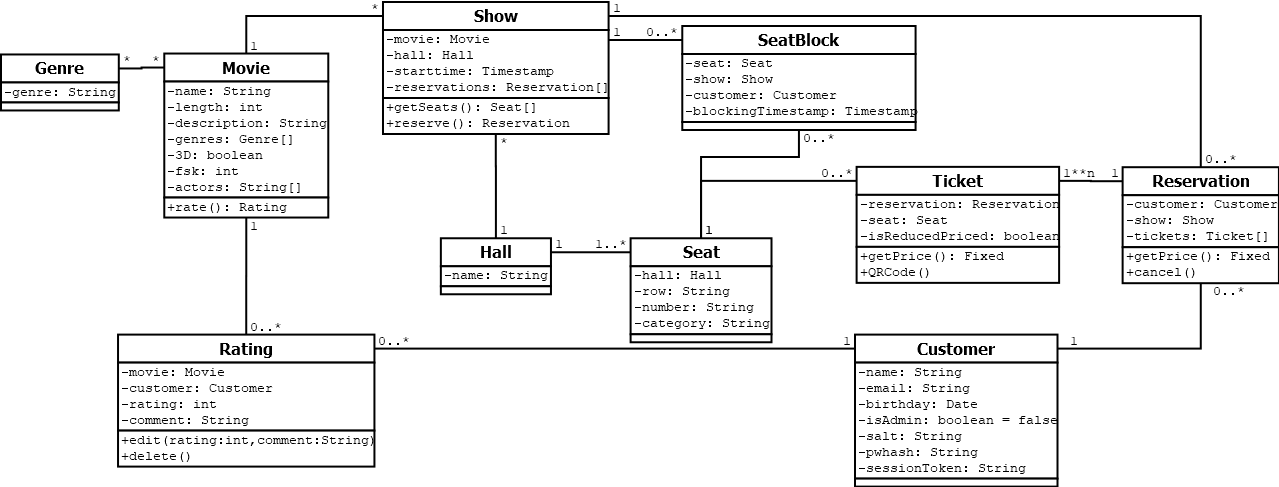
\includegraphics[keepaspectratio, width=\textwidth, height=\textheight]{img/klassendiagramm_v01}
	\captionsetup{format=hang}
	\caption{Erster Entwurf des Klassendiagramms}
	\small Quelle: eigene Darstellung mittels \url{http://dia-installer.de/index.html.de}
	\label{fig:anhang_klassendiagramm01}
\end{sidewaysfigure}

\begin{sidewaysfigure}[ht]
	\centering
	
\includegraphics[keepaspectratio, width=\textwidth, height=\textheight]{img/klassendiagramm_v02}
	\captionsetup{format=hang}
	\caption{Zweiter Entwurf des Klassendiagramms}
	\small Quelle: eigene Darstellung mittels \url{https://draw.io/} 
	\label{fig:anhang_klassendiagramm02}
\end{sidewaysfigure}

\begin{sidewaysfigure}[ht]
	\centering
	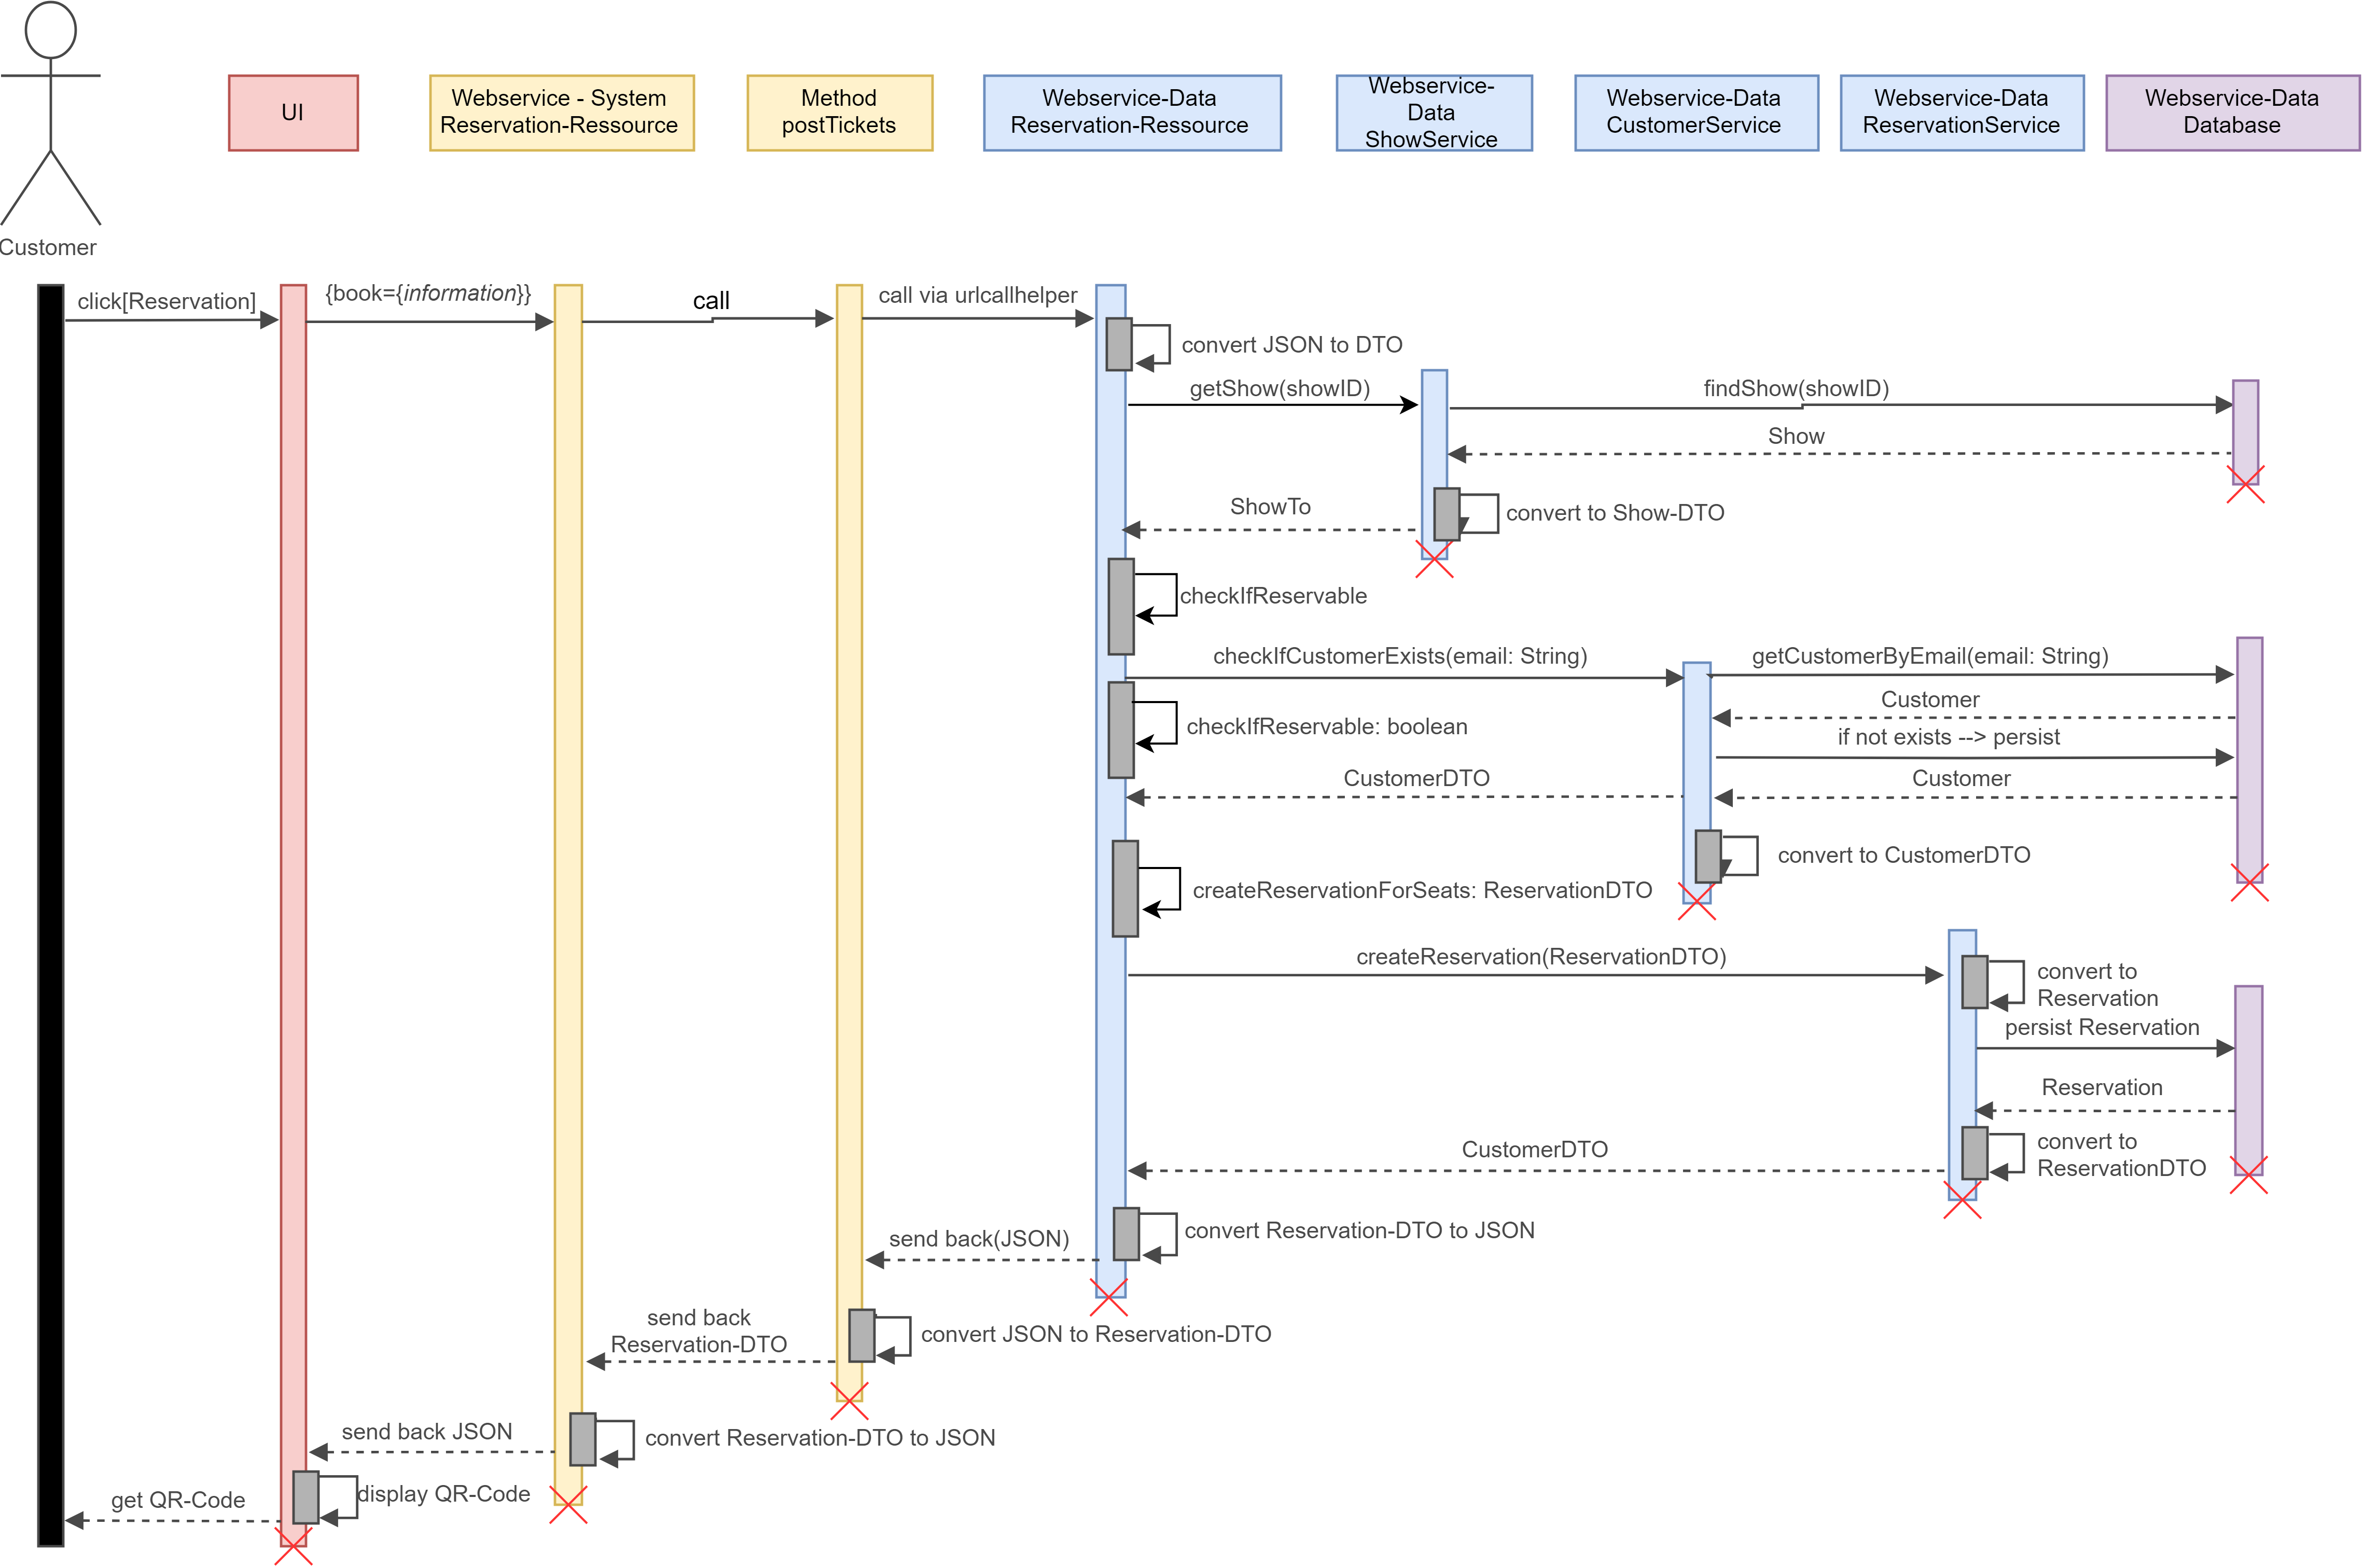
\includegraphics[keepaspectratio, width=\textwidth, height=\textheight]{img/sequenzdiagramm_reservation}
	\captionsetup{format=hang}
	\caption{Sequenzdiagramm eines Reservierungsvorganges}
	\small Quelle: eigene Darstellung mittels \url{https://draw.io/} 
	\label{fig:Anhang_seq_reservieren}
\end{sidewaysfigure}

\begin{sidewaysfigure}[ht]
	\centering
	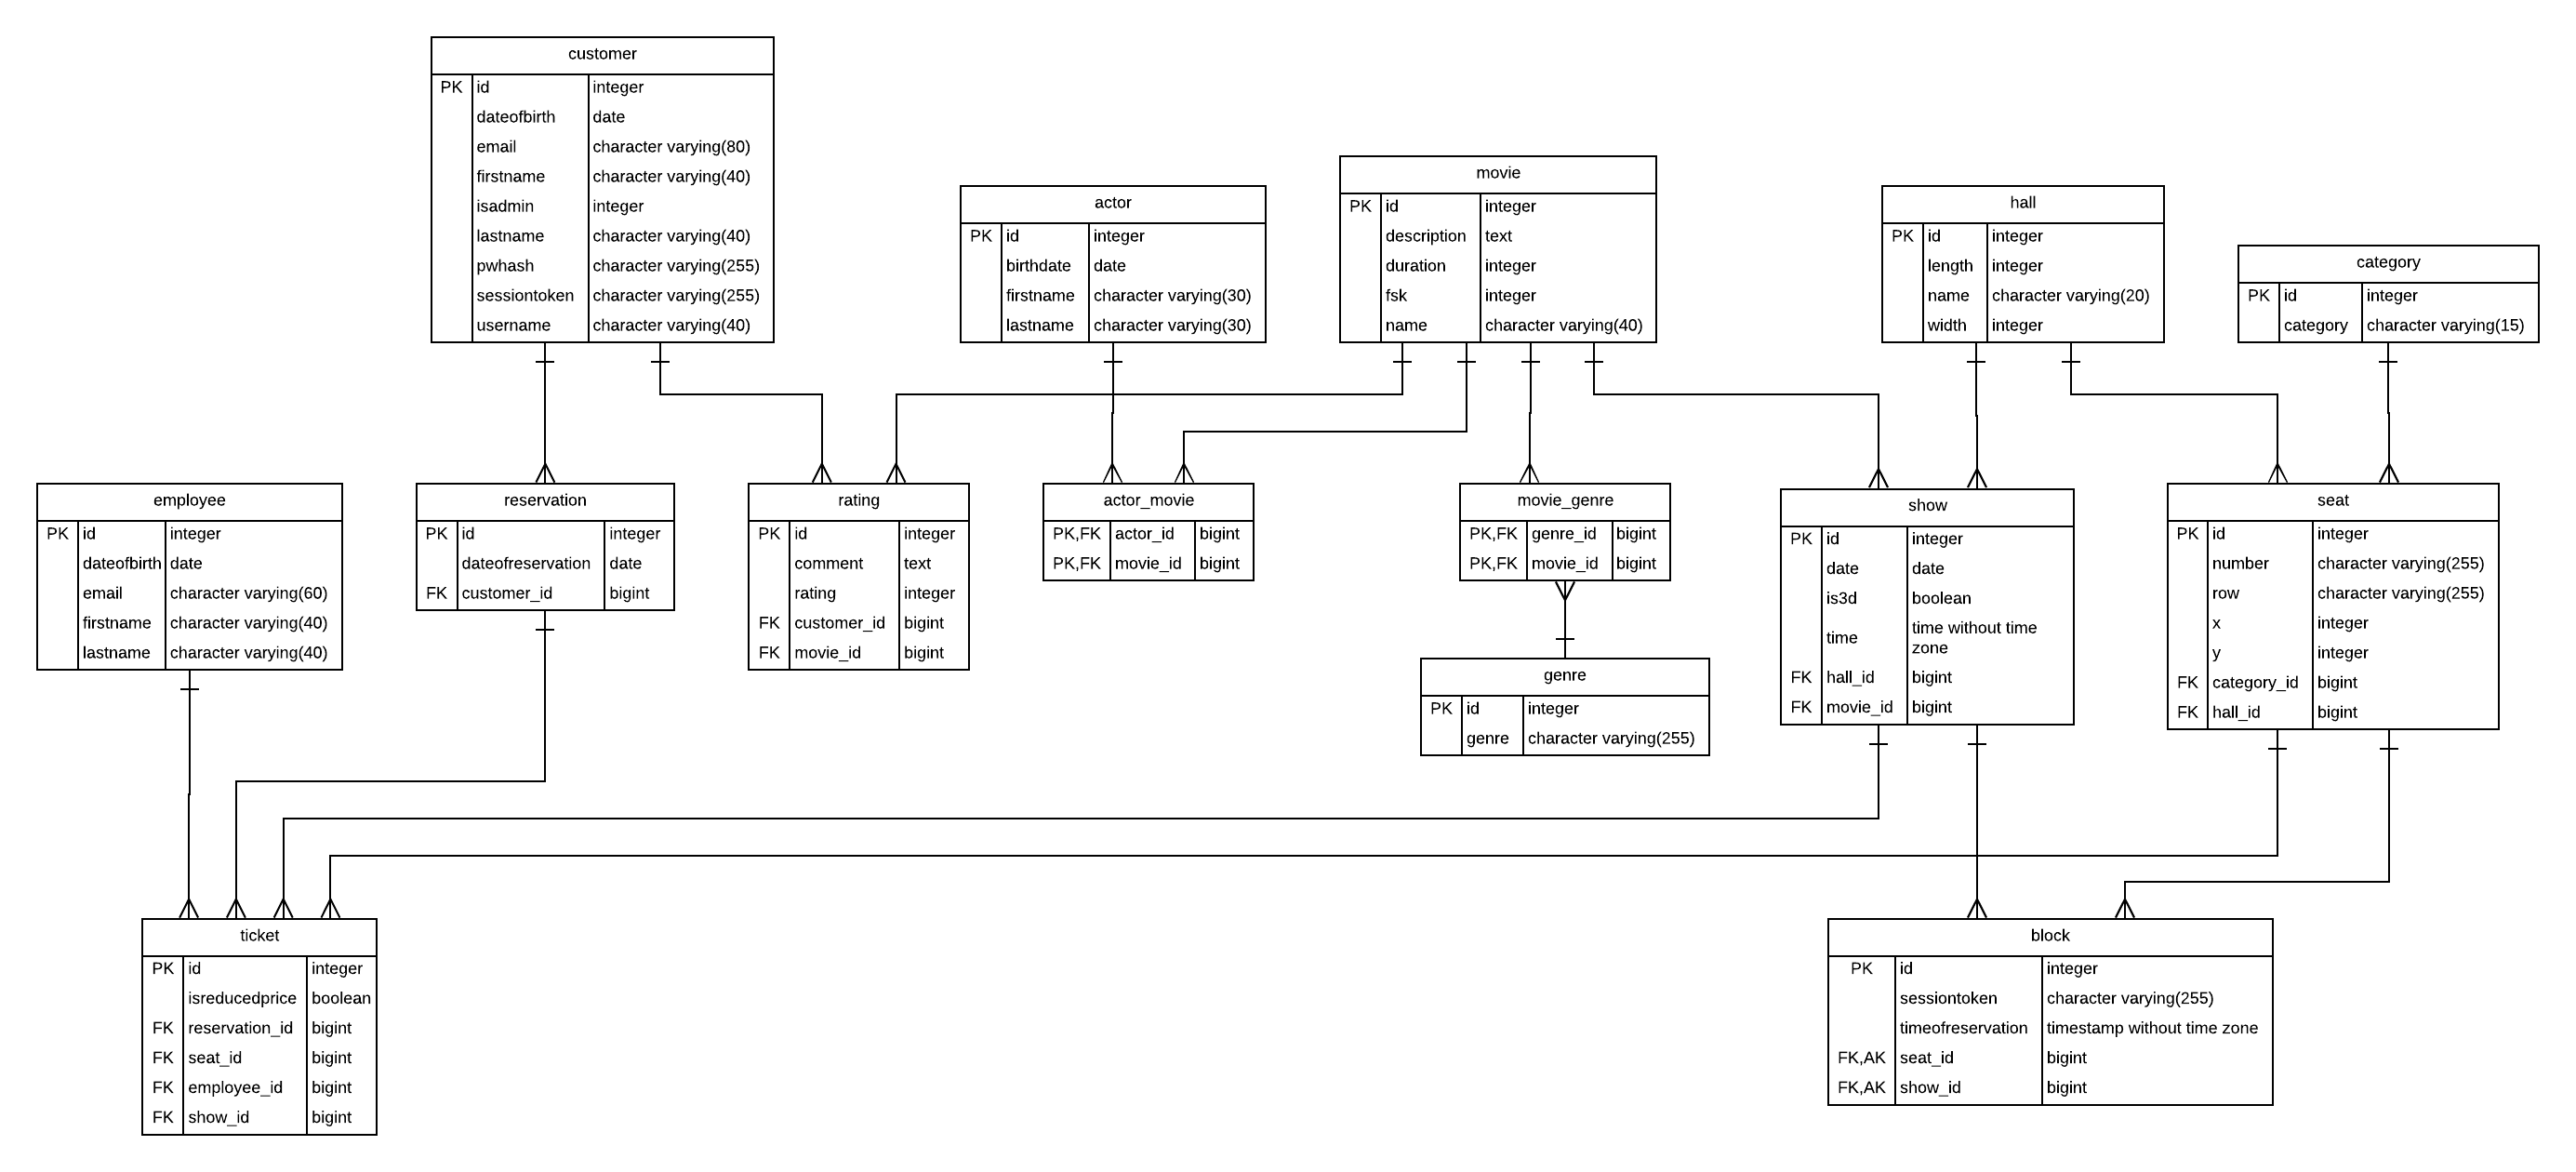
\includegraphics[keepaspectratio, width=\textwidth, height=\textheight]{img/ER-Modell}
	\captionsetup{format=hang}
	\caption{\acs{ER-Modell} der Datenbank}
	\small Quelle: eigene Darstellung mittels \url{https://www.lucidchart.com/}
	\label{fig:Anhang_ER-Modell}
\end{sidewaysfigure}

\chapter{Screenshots aus dem Front-End}
\label{sec:screenshots_frontend}
Die folgenden Screenshots sind alle von der Seite eines Filmes, auf der sich weitere Details zu diesem finden.

\begin{figure}[ht]
	\centering
	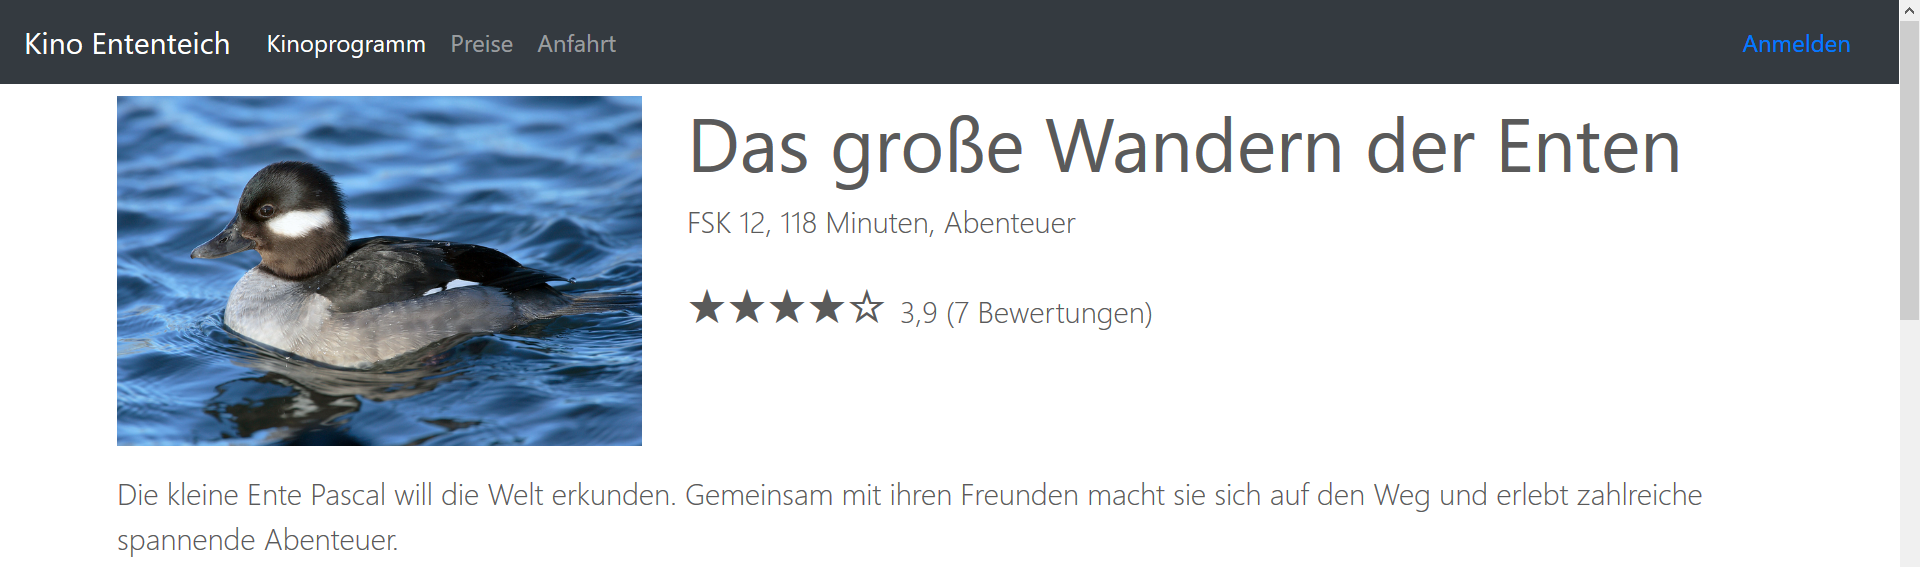
\includegraphics[width=\textwidth]{img/screenshots/film02a}
	\captionsetup{format=hang}
	\caption{Filmdetails}
	\label{fig:film02a}
\end{figure}

\begin{figure}[ht]
	\centering
	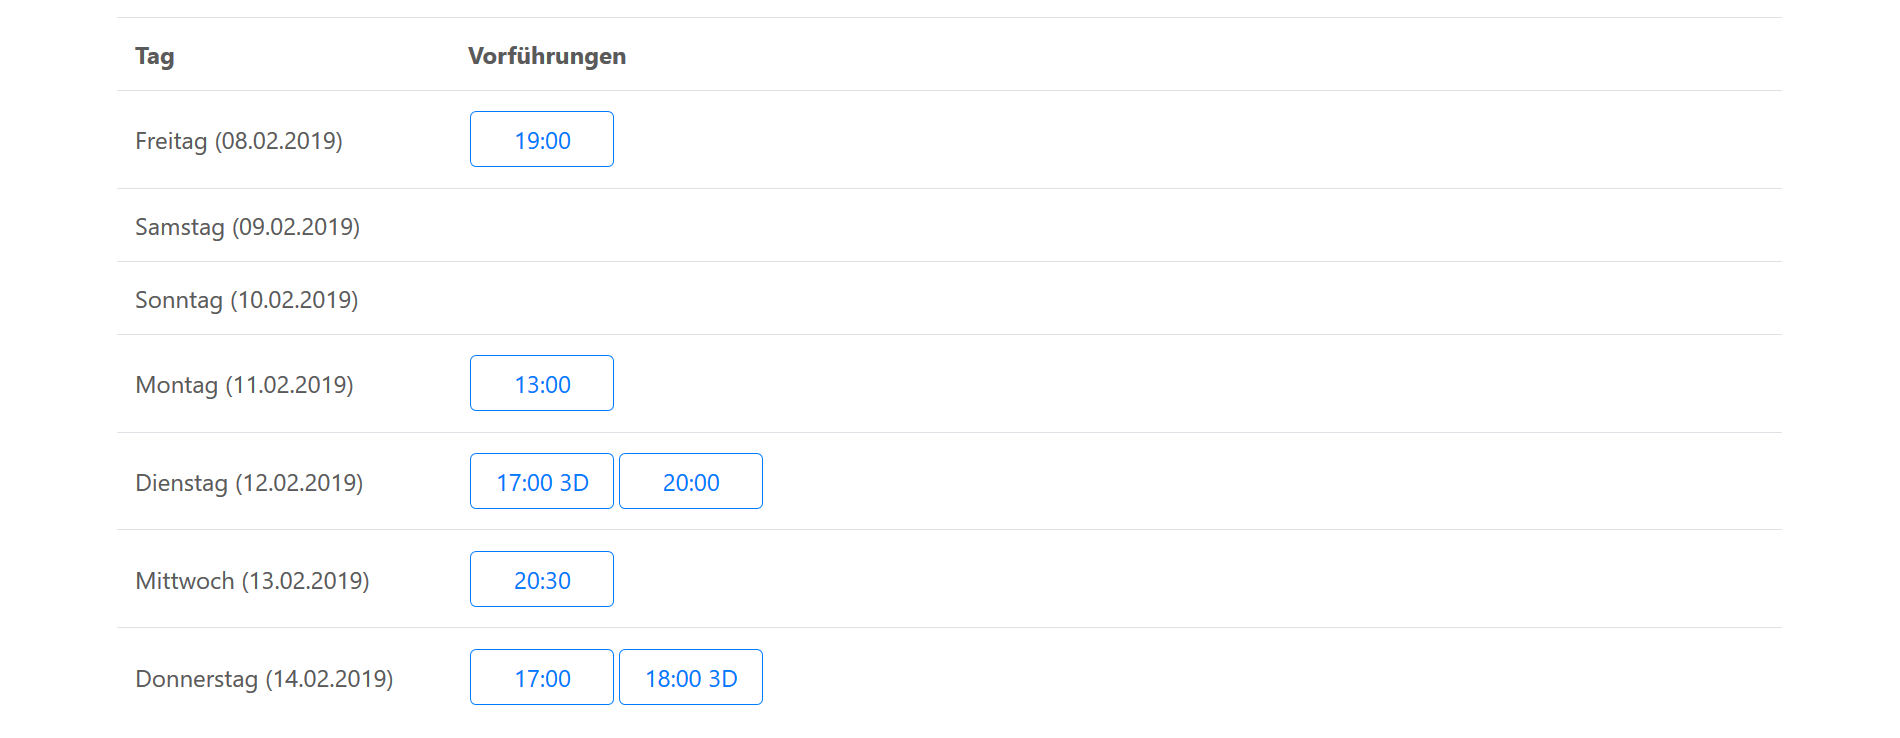
\includegraphics[width=\textwidth]{img/screenshots/film03}
	\captionsetup{format=hang}
	\caption{Liste der Vorstellungen der nächsten 7 Tage}
	\label{fig:film03}
\end{figure}

\begin{figure}[!t]
	\centering
	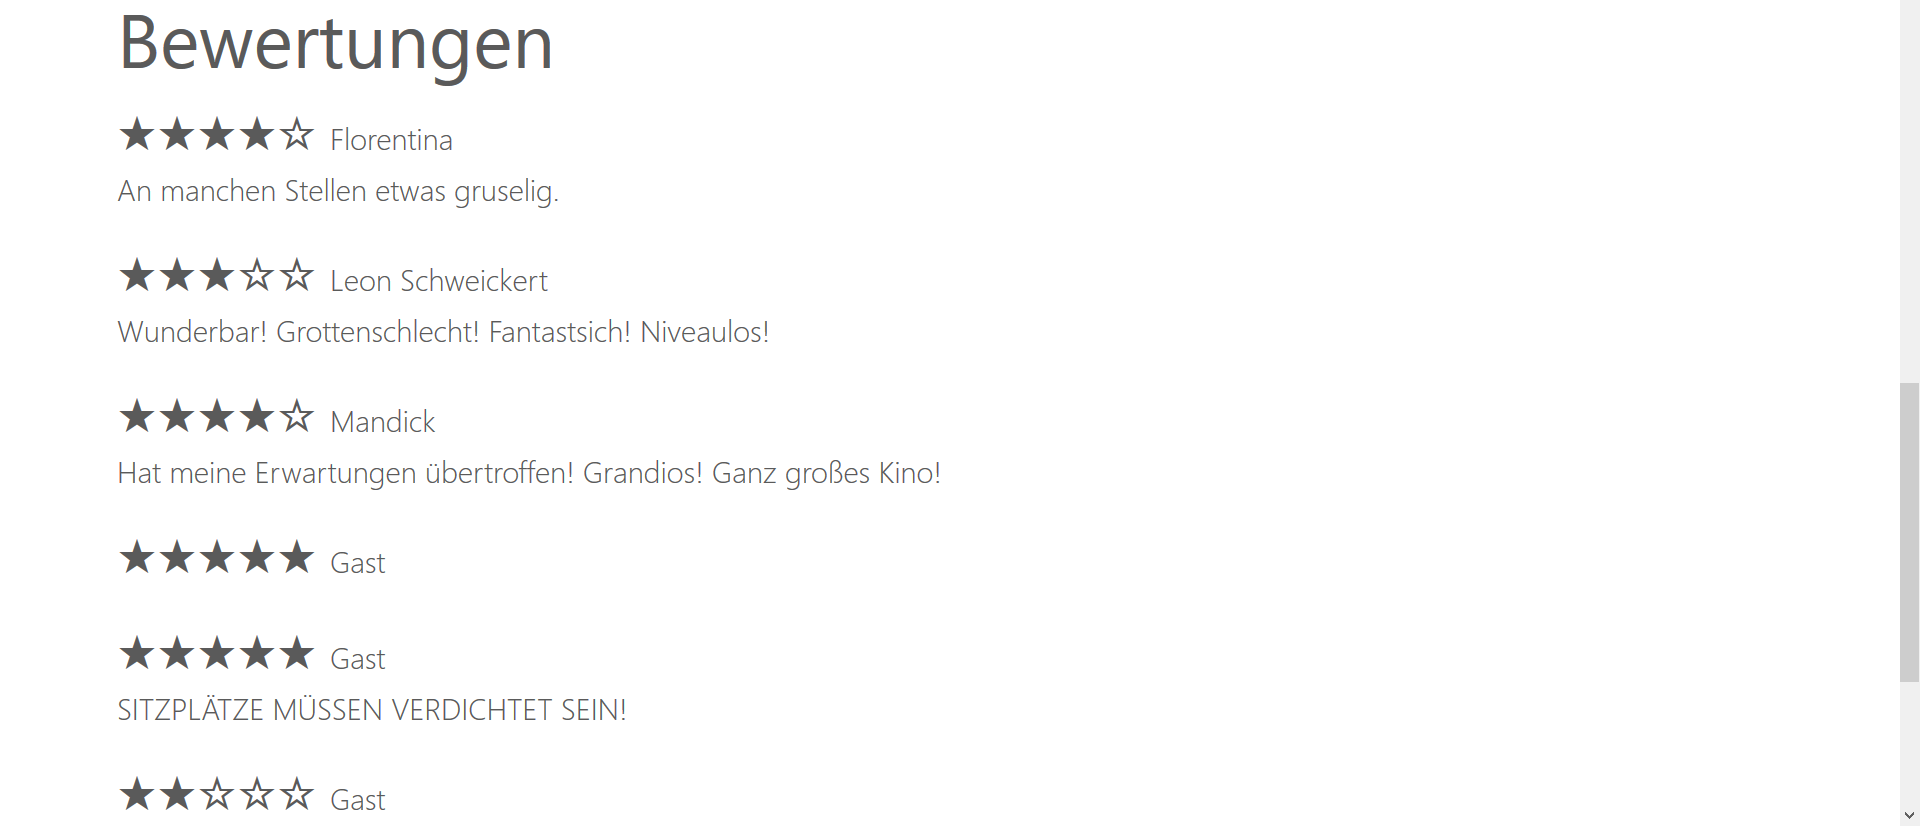
\includegraphics[width=\textwidth]{img/screenshots/film04}
	\captionsetup{format=hang}
	\caption{Bewertungen zu einem Film}
	\label{fig:film04}
\end{figure}

\chapter{Quellcode}

\begin{lstlisting}[style=lstJava, caption={Erstellen eines Movie-\acs{DTO}s aus einer Movie-Entität mit Hilfe des eigen erstellten EntityToToHelper}, label={lst:EntityToToHelper_movie}]
public static MovieTo createMovieTo ( Movie entity, boolean withShow )
{
	if ( null != entity )
	{
		MovieTo movieTo = new MovieTo();
		movieTo.setId(entity.getId());
		movieTo.setDescription(entity.getDescription());
		movieTo.setFsk(entity.getFsk());
		movieTo.setDuration(entity.getDuration());
		movieTo.setName(entity.getName());
		movieTo.setGenres(createGenreTos(entity.getGenres()));
		movieTo.setRatings(createRatingTos(entity.getRatings()));
		if ( withShow )
		{
			movieTo.setShows(createShowTos(entity.getShows(), false));
		} // end withSow
		movieTo.setActors(createActorTos(entity.getActors()));
		return movieTo;
	}  // end if null
	return null;
}
\end{lstlisting}

\newpage

\begin{lstlisting}[style=lstJava, caption={Erstellen einer Movie-Entität aus einem Movie-\acs{DTO} mit Hilfe des eigen erstellten ToToEntityHelper}, label={lst:ToToEntityHelper_movie}]
public static Movie createMovieEntity ( MovieTo transferObject, boolean withShow )
{
	if ( null != transferObject )
	{
		Movie movie = new Movie();
		movie.setId(transferObject.getId());
		movie.setActors(createActorEntities(transferObject.getActors()));
		movie.setDescription(transferObject.getDescription());
		movie.setFsk(transferObject.getFsk());
		movie.setDuration(transferObject.getDuration());
		movie.setName(transferObject.getName());
		movie.setRatings(createRatingEntities(transferObject.getRatings()));
		if ( withShow )
		{
			movie.setShows(createShowEntities(transferObject.getShows(), false));
		}
		movie.setGenres(createGenreEntities(transferObject.getGenres()));
		return movie;
	}
	return null;
}
\end{lstlisting}

\newpage

\begin{lstlisting}[style=lstJava, caption={Überprüfung, ob eine Reservierung möglich ist}, label={lst:Angang_Prüfung_ob_Reservierung_möglich}, tabsize=2]
private boolean checkIfSeatsAreBookable ( List<SeatTo> seatsToProof, List<TicketTo> bookedTicketTos, List<BlockTo> blockTos, String sessiontoken ) {
	boolean bookable = true;
	
	for ( SeatTo s : seatsToProof ) {
		if ( bookable ) {
			for ( TicketTo t : bookedTicketTos ) {
				if ( s.getId() == t.getSeat().getId() ) {
					bookable = false;
					s.setOccupied(true);
					break;
				}
				else {
					s.setOccupied(false);
				}
			} // end for ticket

			// verification for blocked elements
			for ( BlockTo b : blockTos ) {
				if ( s.getId() == b.getSeat().getId() &&
				     !(b.getSessiontoken().equals(sessiontoken)) ) {
					bookable = false;
					s.setBlocked(true);
					break;
				}
				else {
					s.setBlocked(false);
				}
			} // end for block
		}	// end if bookable
	}	// end for seatTo

	return bookable;
}
\end{lstlisting}

\newpage

\begin{lstlisting}[style=lstJava, caption={Erstellen eines Reservierungs-\acs{DTO}s}, label={lst:Anhang_Erstellen_Reservierung}]
private ReservationTo createReservationForSeats ( List<SeatTo> seatTos, ShowTo showTo )
{
	List<TicketTo> toBook = new ArrayList<>();
	ReservationTo createdReservationTo = new ReservationTo();
		
	for ( SeatTo seatTo : seatTos )
	{
		seatTo.setOccupied(true);
	
		TicketTo ticketTo = new TicketTo();
		ticketTo.setSeat(seatTo);
		ticketTo.setShow(showTo);
		ticketTo.setReservation(createdReservationTo);
		if ( seatTo.isReducedPrice() )
		{
			ticketTo.setReducedPrice(true);
		}
		toBook.add(ticketTo);
	}
	createdReservationTo.setDateOfReservation(Utils.convertDateToString(new Date()));
	createdReservationTo.setTickets(toBook);
	return createdReservationTo;
}
\end{lstlisting}

\newpage

\begin{lstlisting}[style=lstJava, caption={Ausschnitt der Test-Klasse der EntityToToHelper-Klasse}, label={src:entitytotohelpertest}, tabsize=2]
public class EntityToToHelper_Test {
	EntityToToHelper EtoToHelper = new EntityToToHelper();

	@Before
	public void initialize ( ) {
		EmployeeTo testEmployeeTo = new EmployeeTo();
		testEmployeeTo.setId(1);
		testEmployeeTo.setDateofbirth(testDateString);
		testEmployeeTo.setEmail("mail");
		testEmployeeTo.setFirstname("firstname");
		testEmployeeTo.setLastname("lastname");

		Employee testEmployeeEntity = new Employee();
		testEmployeeEntity.setId(1);
		testEmployeeEntity.setDateofbirth(testDateDate);
		testEmployeeEntity.setEmail("mail");
		testEmployeeEntity.setFirstname("firstname");
		testEmployeeEntity.setLastname("lastname");
	}

	@Test
	public void testCreateEmployeeTo ( ) {
		assertEquals(null, EtoToHelper.createEmployeeTo(null));

		EmployeeTo compareEmployeeTo = EtoToHelper.createEmployeeTo(testEmployeeEntity);

		assertThat(testEmployeeTo.getId(), equalTo(compareEmployeeTo.getId()));
		assertThat(testEmployeeTo.getDateofbirth(), equalTo(compareEmployeeTo.getDateofbirth()));
		assertThat(testEmployeeTo.getEmail(), equalTo(compareEmployeeTo.getEmail()));
		assertThat(testEmployeeTo.getFirstname(), equalTo(compareEmployeeTo.getFirstname()));
		assertThat(testEmployeeTo.getLastname(), equalTo(compareEmployeeTo.getLastname()));
	}
}
\end{lstlisting}


% ewerkl.tex
%% !TEX root =  master.tex

\clearpage
\chapter*{Ehrenwörtliche Erklärung}

Wir versichern hiermit, dass wir die vorliegende Arbeit mit dem Thema \textit{\DerTitelDerArbeit} selbstständig verfasst und keine anderen als die angegebenen Quellen und Hilfsmittel benutzt haben.
%Wir versichern zudem, dass die eingereichte elektronische Fassung mit der gedruckten Fassung übereinstimmt.

\vspace{2cm}
Mannheim, den 09.06.2020

\vspace{1cm}

\begin{table}[h!]
	\setlength\tabcolsep{0pt}
	\renewcommand{\arraystretch}{1.4}
	\begin{tabular}{L{5.1cm}C{5.1cm}R{5.1cm}}
		\authorSG & \authorRF & \authorMS \\
		& & \\
		\authorEJ & \authorNL & \authorJR \\
	\end{tabular}
\end{table}

\includepdf[pages={99}]{Seminararbeit_KinoEntenteich_unterschrieben.pdf}


\end{document}
